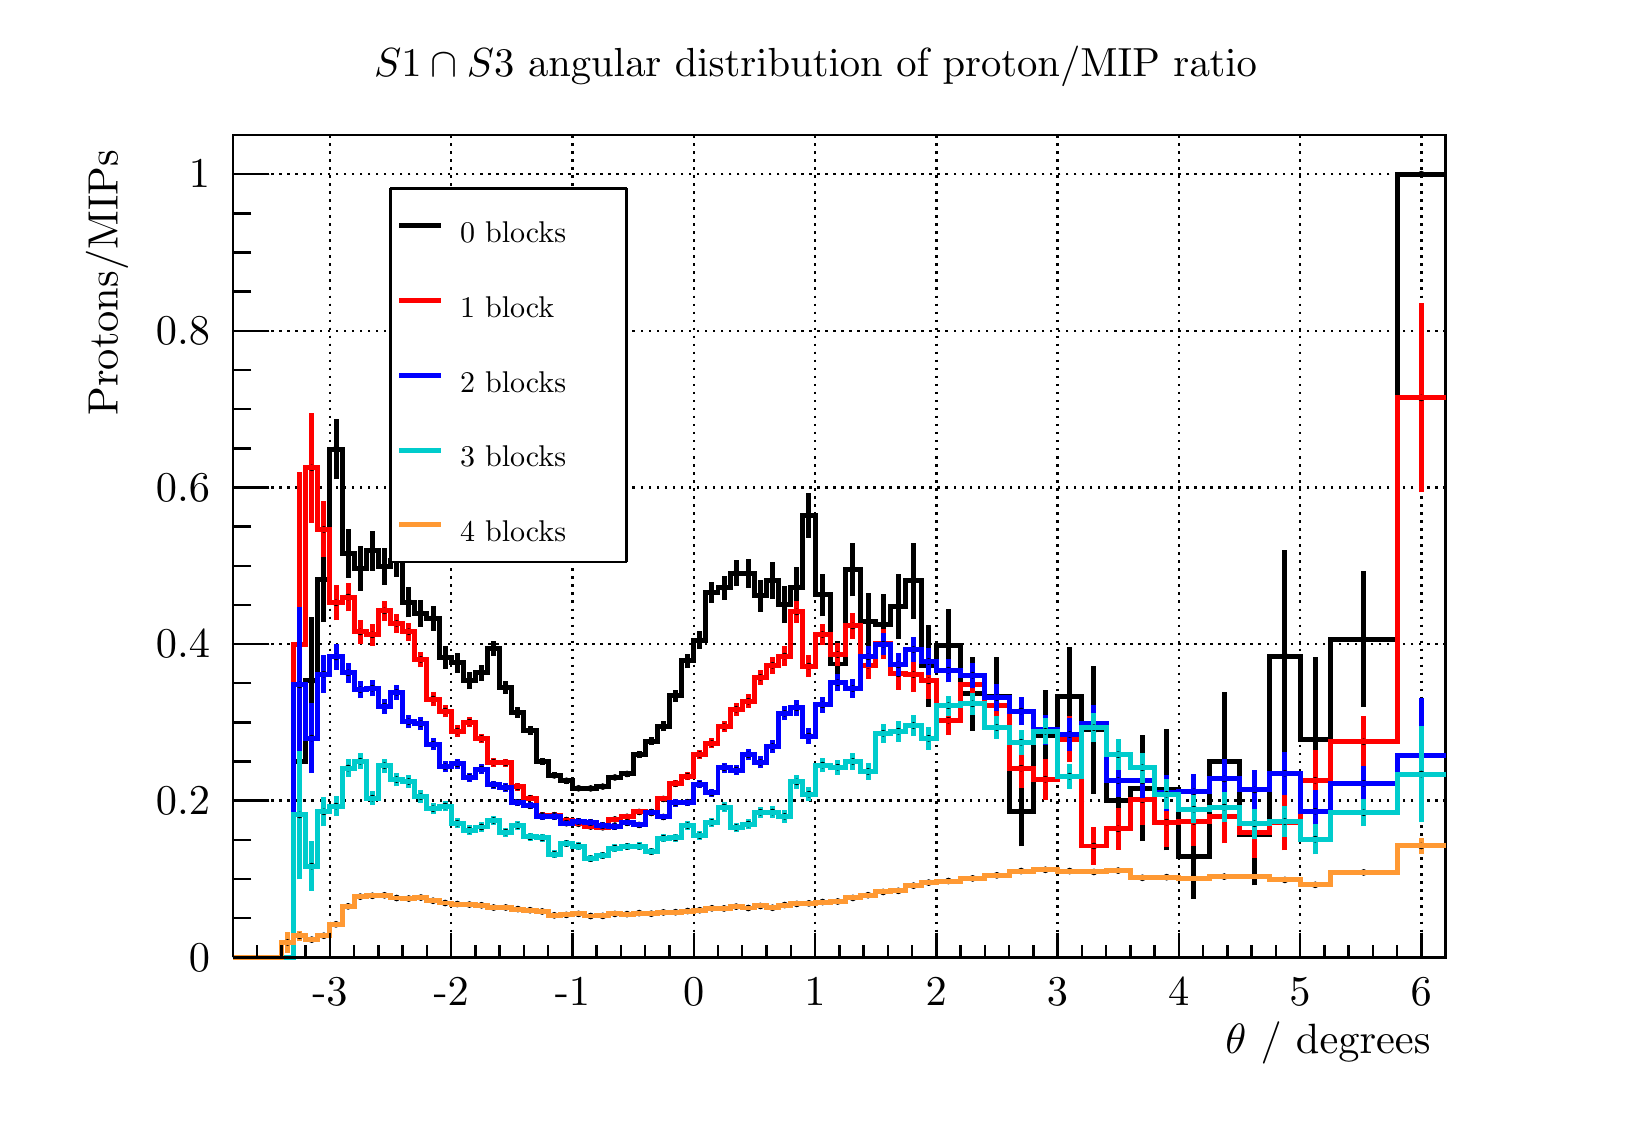
\begin{tikzpicture}
\pgfdeclareplotmark{cross} {
\pgfpathmoveto{\pgfpoint{-0.3\pgfplotmarksize}{\pgfplotmarksize}}
\pgfpathlineto{\pgfpoint{+0.3\pgfplotmarksize}{\pgfplotmarksize}}
\pgfpathlineto{\pgfpoint{+0.3\pgfplotmarksize}{0.3\pgfplotmarksize}}
\pgfpathlineto{\pgfpoint{+1\pgfplotmarksize}{0.3\pgfplotmarksize}}
\pgfpathlineto{\pgfpoint{+1\pgfplotmarksize}{-0.3\pgfplotmarksize}}
\pgfpathlineto{\pgfpoint{+0.3\pgfplotmarksize}{-0.3\pgfplotmarksize}}
\pgfpathlineto{\pgfpoint{+0.3\pgfplotmarksize}{-1.\pgfplotmarksize}}
\pgfpathlineto{\pgfpoint{-0.3\pgfplotmarksize}{-1.\pgfplotmarksize}}
\pgfpathlineto{\pgfpoint{-0.3\pgfplotmarksize}{-0.3\pgfplotmarksize}}
\pgfpathlineto{\pgfpoint{-1.\pgfplotmarksize}{-0.3\pgfplotmarksize}}
\pgfpathlineto{\pgfpoint{-1.\pgfplotmarksize}{0.3\pgfplotmarksize}}
\pgfpathlineto{\pgfpoint{-0.3\pgfplotmarksize}{0.3\pgfplotmarksize}}
\pgfpathclose
\pgfusepathqstroke
}
\pgfdeclareplotmark{cross*} {
\pgfpathmoveto{\pgfpoint{-0.3\pgfplotmarksize}{\pgfplotmarksize}}
\pgfpathlineto{\pgfpoint{+0.3\pgfplotmarksize}{\pgfplotmarksize}}
\pgfpathlineto{\pgfpoint{+0.3\pgfplotmarksize}{0.3\pgfplotmarksize}}
\pgfpathlineto{\pgfpoint{+1\pgfplotmarksize}{0.3\pgfplotmarksize}}
\pgfpathlineto{\pgfpoint{+1\pgfplotmarksize}{-0.3\pgfplotmarksize}}
\pgfpathlineto{\pgfpoint{+0.3\pgfplotmarksize}{-0.3\pgfplotmarksize}}
\pgfpathlineto{\pgfpoint{+0.3\pgfplotmarksize}{-1.\pgfplotmarksize}}
\pgfpathlineto{\pgfpoint{-0.3\pgfplotmarksize}{-1.\pgfplotmarksize}}
\pgfpathlineto{\pgfpoint{-0.3\pgfplotmarksize}{-0.3\pgfplotmarksize}}
\pgfpathlineto{\pgfpoint{-1.\pgfplotmarksize}{-0.3\pgfplotmarksize}}
\pgfpathlineto{\pgfpoint{-1.\pgfplotmarksize}{0.3\pgfplotmarksize}}
\pgfpathlineto{\pgfpoint{-0.3\pgfplotmarksize}{0.3\pgfplotmarksize}}
\pgfpathclose
\pgfusepathqfillstroke
}
\pgfdeclareplotmark{newstar} {
\pgfpathmoveto{\pgfqpoint{0pt}{\pgfplotmarksize}}
\pgfpathlineto{\pgfqpointpolar{44}{0.5\pgfplotmarksize}}
\pgfpathlineto{\pgfqpointpolar{18}{\pgfplotmarksize}}
\pgfpathlineto{\pgfqpointpolar{-20}{0.5\pgfplotmarksize}}
\pgfpathlineto{\pgfqpointpolar{-54}{\pgfplotmarksize}}
\pgfpathlineto{\pgfqpointpolar{-90}{0.5\pgfplotmarksize}}
\pgfpathlineto{\pgfqpointpolar{234}{\pgfplotmarksize}}
\pgfpathlineto{\pgfqpointpolar{198}{0.5\pgfplotmarksize}}
\pgfpathlineto{\pgfqpointpolar{162}{\pgfplotmarksize}}
\pgfpathlineto{\pgfqpointpolar{134}{0.5\pgfplotmarksize}}
\pgfpathclose
\pgfusepathqstroke
}
\pgfdeclareplotmark{newstar*} {
\pgfpathmoveto{\pgfqpoint{0pt}{\pgfplotmarksize}}
\pgfpathlineto{\pgfqpointpolar{44}{0.5\pgfplotmarksize}}
\pgfpathlineto{\pgfqpointpolar{18}{\pgfplotmarksize}}
\pgfpathlineto{\pgfqpointpolar{-20}{0.5\pgfplotmarksize}}
\pgfpathlineto{\pgfqpointpolar{-54}{\pgfplotmarksize}}
\pgfpathlineto{\pgfqpointpolar{-90}{0.5\pgfplotmarksize}}
\pgfpathlineto{\pgfqpointpolar{234}{\pgfplotmarksize}}
\pgfpathlineto{\pgfqpointpolar{198}{0.5\pgfplotmarksize}}
\pgfpathlineto{\pgfqpointpolar{162}{\pgfplotmarksize}}
\pgfpathlineto{\pgfqpointpolar{134}{0.5\pgfplotmarksize}}
\pgfpathclose
\pgfusepathqfillstroke
}
\definecolor{c}{rgb}{1,1,1};
\draw [color=c, fill=c] (0,0) rectangle (20,13.5632);
\draw [color=c, fill=c] (2.6,1.76322) rectangle (18,12.2069);
\definecolor{c}{rgb}{0,0,0};
\draw [c,line width=0.9] (2.6,1.76322) -- (2.6,12.2069) -- (18,12.2069) -- (18,1.76322) -- (2.6,1.76322);
\definecolor{c}{rgb}{1,1,1};
\draw [color=c, fill=c] (2.6,1.76322) rectangle (18,12.2069);
\definecolor{c}{rgb}{0,0,0};
\draw [c,line width=0.9] (2.6,1.76322) -- (2.6,12.2069) -- (18,12.2069) -- (18,1.76322) -- (2.6,1.76322);
\draw [c,line width=0.9] (2.6,1.76322) -- (18,1.76322);
\draw [c,dotted,line width=0.9] (3.832,12.2069) -- (3.832,1.76322);
\draw [c,dotted,line width=0.9] (5.372,12.2069) -- (5.372,1.76322);
\draw [c,dotted,line width=0.9] (6.912,12.2069) -- (6.912,1.76322);
\draw [c,dotted,line width=0.9] (8.452,12.2069) -- (8.452,1.76322);
\draw [c,dotted,line width=0.9] (9.992,12.2069) -- (9.992,1.76322);
\draw [c,dotted,line width=0.9] (11.532,12.2069) -- (11.532,1.76322);
\draw [c,dotted,line width=0.9] (13.072,12.2069) -- (13.072,1.76322);
\draw [c,dotted,line width=0.9] (14.612,12.2069) -- (14.612,1.76322);
\draw [c,dotted,line width=0.9] (16.152,12.2069) -- (16.152,1.76322);
\draw [c,dotted,line width=0.9] (17.692,12.2069) -- (17.692,1.76322);
\draw [c,dotted,line width=0.9] (3.832,12.2069) -- (3.832,1.76322);
\draw [c,dotted,line width=0.9] (17.692,12.2069) -- (17.692,1.76322);
\draw [c,line width=0.9] (2.6,1.76322) -- (2.6,12.2069);
\draw [c,dotted,line width=0.9] (18,1.76322) -- (2.6,1.76322);
\draw [c,dotted,line width=0.9] (18,3.75249) -- (2.6,3.75249);
\draw [c,dotted,line width=0.9] (18,5.74176) -- (2.6,5.74176);
\draw [c,dotted,line width=0.9] (18,7.73103) -- (2.6,7.73103);
\draw [c,dotted,line width=0.9] (18,9.72031) -- (2.6,9.72031);
\draw [c,dotted,line width=0.9] (18,11.7096) -- (2.6,11.7096);
\draw [c,dotted,line width=0.9] (18,11.7096) -- (2.6,11.7096);
\definecolor{c}{rgb}{0,0,0.6};
\draw [c,line width=0.9] (2.6,1.76322) -- (2.754,1.76322) -- (2.754,1.76322) -- (2.908,1.76322) -- (2.908,1.76322) -- (3.062,1.76322) -- (3.062,1.76322) -- (3.216,1.76322) -- (3.216,1.76322) -- (3.37,1.76322) -- (3.37,1.76322) -- (3.524,1.76322) --
 (3.524,1.76322) -- (3.678,1.76322) -- (3.678,1.76322) -- (3.832,1.76322) -- (3.832,1.76322) -- (3.986,1.76322) -- (3.986,1.76322) -- (4.14,1.76322) -- (4.14,1.76322) -- (4.294,1.76322) -- (4.294,1.76322) -- (4.448,1.76322) -- (4.448,1.76322) --
 (4.602,1.76322) -- (4.602,1.76322) -- (4.756,1.76322) -- (4.756,1.76322) -- (4.91,1.76322) -- (4.91,1.76322) -- (5.064,1.76322) -- (5.064,1.76322) -- (5.218,1.76322) -- (5.218,1.76322) -- (5.372,1.76322) -- (5.372,1.76322) -- (5.526,1.76322) --
 (5.526,1.76322) -- (5.68,1.76322) -- (5.68,1.76322) -- (5.834,1.76322) -- (5.834,1.76322) -- (5.988,1.76322) -- (5.988,1.76322) -- (6.142,1.76322) -- (6.142,1.76322) -- (6.296,1.76322) -- (6.296,1.76322) -- (6.45,1.76322) -- (6.45,1.76322) --
 (6.604,1.76322) -- (6.604,1.76322) -- (6.758,1.76322) -- (6.758,1.76322) -- (6.912,1.76322) -- (6.912,1.76322) -- (7.066,1.76322) -- (7.066,1.76322) -- (7.22,1.76322) -- (7.22,1.76322) -- (7.374,1.76322) -- (7.374,1.76322) -- (7.528,1.76322) --
 (7.528,1.76322) -- (7.682,1.76322) -- (7.682,1.76322) -- (7.836,1.76322) -- (7.836,1.76322) -- (7.99,1.76322) -- (7.99,1.76322) -- (8.144,1.76322) -- (8.144,1.76322) -- (8.298,1.76322) -- (8.298,1.76322) -- (8.452,1.76322) -- (8.452,1.76322) --
 (8.606,1.76322) -- (8.606,1.76322) -- (8.76,1.76322) -- (8.76,1.76322) -- (8.914,1.76322) -- (8.914,1.76322) -- (9.068,1.76322) -- (9.068,1.76322) -- (9.222,1.76322) -- (9.222,1.76322) -- (9.376,1.76322) -- (9.376,1.76322) -- (9.53,1.76322) --
 (9.53,1.76322) -- (9.684,1.76322) -- (9.684,1.76322) -- (9.838,1.76322) -- (9.838,1.76322) -- (9.992,1.76322) -- (9.992,1.76322) -- (10.1845,1.76322) -- (10.1845,1.76322) -- (10.377,1.76322) -- (10.377,1.76322) -- (10.5695,1.76322) --
 (10.5695,1.76322) -- (10.762,1.76322) -- (10.762,1.76322) -- (10.9545,1.76322) -- (10.9545,1.76322) -- (11.147,1.76322) -- (11.147,1.76322) -- (11.3395,1.76322) -- (11.3395,1.76322) -- (11.532,1.76322) -- (11.532,1.76322) -- (11.84,1.76322) --
 (11.84,1.76322) -- (12.148,1.76322) -- (12.148,1.76322) -- (12.456,1.76322) -- (12.456,1.76322) -- (12.764,1.76322) -- (12.764,1.76322) -- (13.072,1.76322) -- (13.072,1.76322) -- (13.38,1.76322) -- (13.38,1.76322) -- (13.688,1.76322) --
 (13.688,1.76322) -- (13.996,1.76322) -- (13.996,1.76322) -- (14.304,1.76322) -- (14.304,1.76322) -- (14.612,1.76322) -- (14.612,1.76322) -- (14.997,1.76322) -- (14.997,1.76322) -- (15.382,1.76322) -- (15.382,1.76322) -- (15.767,1.76322) --
 (15.767,1.76322) -- (16.152,1.76322) -- (16.152,1.76322) -- (16.537,1.76322) -- (16.537,1.76322) -- (17.384,1.76322) -- (17.384,1.76322) -- (18,1.76322);
\definecolor{c}{rgb}{0,0,0};
\draw [c,line width=0.9] (2.6,1.76322) -- (18,1.76322);
\draw [anchor= east] (18,0.678161) node[scale=1.5317, color=c, rotate=0]{$\theta$ / degrees};
\draw [c,line width=0.9] (3.832,2.07653) -- (3.832,1.76322);
\draw [c,line width=0.9] (4.14,1.91987) -- (4.14,1.76322);
\draw [c,line width=0.9] (4.448,1.91987) -- (4.448,1.76322);
\draw [c,line width=0.9] (4.756,1.91987) -- (4.756,1.76322);
\draw [c,line width=0.9] (5.064,1.91987) -- (5.064,1.76322);
\draw [c,line width=0.9] (5.372,2.07653) -- (5.372,1.76322);
\draw [c,line width=0.9] (5.68,1.91987) -- (5.68,1.76322);
\draw [c,line width=0.9] (5.988,1.91987) -- (5.988,1.76322);
\draw [c,line width=0.9] (6.296,1.91987) -- (6.296,1.76322);
\draw [c,line width=0.9] (6.604,1.91987) -- (6.604,1.76322);
\draw [c,line width=0.9] (6.912,2.07653) -- (6.912,1.76322);
\draw [c,line width=0.9] (7.22,1.91987) -- (7.22,1.76322);
\draw [c,line width=0.9] (7.528,1.91987) -- (7.528,1.76322);
\draw [c,line width=0.9] (7.836,1.91987) -- (7.836,1.76322);
\draw [c,line width=0.9] (8.144,1.91987) -- (8.144,1.76322);
\draw [c,line width=0.9] (8.452,2.07653) -- (8.452,1.76322);
\draw [c,line width=0.9] (8.76,1.91987) -- (8.76,1.76322);
\draw [c,line width=0.9] (9.068,1.91987) -- (9.068,1.76322);
\draw [c,line width=0.9] (9.376,1.91987) -- (9.376,1.76322);
\draw [c,line width=0.9] (9.684,1.91987) -- (9.684,1.76322);
\draw [c,line width=0.9] (9.992,2.07653) -- (9.992,1.76322);
\draw [c,line width=0.9] (10.3,1.91987) -- (10.3,1.76322);
\draw [c,line width=0.9] (10.608,1.91987) -- (10.608,1.76322);
\draw [c,line width=0.9] (10.916,1.91987) -- (10.916,1.76322);
\draw [c,line width=0.9] (11.224,1.91987) -- (11.224,1.76322);
\draw [c,line width=0.9] (11.532,2.07653) -- (11.532,1.76322);
\draw [c,line width=0.9] (11.84,1.91987) -- (11.84,1.76322);
\draw [c,line width=0.9] (12.148,1.91987) -- (12.148,1.76322);
\draw [c,line width=0.9] (12.456,1.91987) -- (12.456,1.76322);
\draw [c,line width=0.9] (12.764,1.91987) -- (12.764,1.76322);
\draw [c,line width=0.9] (13.072,2.07653) -- (13.072,1.76322);
\draw [c,line width=0.9] (13.38,1.91987) -- (13.38,1.76322);
\draw [c,line width=0.9] (13.688,1.91987) -- (13.688,1.76322);
\draw [c,line width=0.9] (13.996,1.91987) -- (13.996,1.76322);
\draw [c,line width=0.9] (14.304,1.91987) -- (14.304,1.76322);
\draw [c,line width=0.9] (14.612,2.07653) -- (14.612,1.76322);
\draw [c,line width=0.9] (14.92,1.91987) -- (14.92,1.76322);
\draw [c,line width=0.9] (15.228,1.91987) -- (15.228,1.76322);
\draw [c,line width=0.9] (15.536,1.91987) -- (15.536,1.76322);
\draw [c,line width=0.9] (15.844,1.91987) -- (15.844,1.76322);
\draw [c,line width=0.9] (16.152,2.07653) -- (16.152,1.76322);
\draw [c,line width=0.9] (16.46,1.91987) -- (16.46,1.76322);
\draw [c,line width=0.9] (16.768,1.91987) -- (16.768,1.76322);
\draw [c,line width=0.9] (17.076,1.91987) -- (17.076,1.76322);
\draw [c,line width=0.9] (17.384,1.91987) -- (17.384,1.76322);
\draw [c,line width=0.9] (17.692,2.07653) -- (17.692,1.76322);
\draw [c,line width=0.9] (3.832,2.07653) -- (3.832,1.76322);
\draw [c,line width=0.9] (3.524,1.91987) -- (3.524,1.76322);
\draw [c,line width=0.9] (3.216,1.91987) -- (3.216,1.76322);
\draw [c,line width=0.9] (2.908,1.91987) -- (2.908,1.76322);
\draw [c,line width=0.9] (17.692,2.07653) -- (17.692,1.76322);
\draw [anchor=base] (3.832,1.15287) node[scale=1.5317, color=c, rotate=0]{-3};
\draw [anchor=base] (5.372,1.15287) node[scale=1.5317, color=c, rotate=0]{-2};
\draw [anchor=base] (6.912,1.15287) node[scale=1.5317, color=c, rotate=0]{-1};
\draw [anchor=base] (8.452,1.15287) node[scale=1.5317, color=c, rotate=0]{0};
\draw [anchor=base] (9.992,1.15287) node[scale=1.5317, color=c, rotate=0]{1};
\draw [anchor=base] (11.532,1.15287) node[scale=1.5317, color=c, rotate=0]{2};
\draw [anchor=base] (13.072,1.15287) node[scale=1.5317, color=c, rotate=0]{3};
\draw [anchor=base] (14.612,1.15287) node[scale=1.5317, color=c, rotate=0]{4};
\draw [anchor=base] (16.152,1.15287) node[scale=1.5317, color=c, rotate=0]{5};
\draw [anchor=base] (17.692,1.15287) node[scale=1.5317, color=c, rotate=0]{6};
\draw [c,line width=0.9] (2.6,1.76322) -- (2.6,12.2069);
\draw [anchor= east] (1,12.2069) node[scale=1.5317, color=c, rotate=90]{  Protons/MIPs};
\draw [c,line width=0.9] (3.062,1.76322) -- (2.6,1.76322);
\draw [c,line width=0.9] (2.831,2.26054) -- (2.6,2.26054);
\draw [c,line width=0.9] (2.831,2.75785) -- (2.6,2.75785);
\draw [c,line width=0.9] (2.831,3.25517) -- (2.6,3.25517);
\draw [c,line width=0.9] (3.062,3.75249) -- (2.6,3.75249);
\draw [c,line width=0.9] (2.831,4.24981) -- (2.6,4.24981);
\draw [c,line width=0.9] (2.831,4.74713) -- (2.6,4.74713);
\draw [c,line width=0.9] (2.831,5.24444) -- (2.6,5.24444);
\draw [c,line width=0.9] (3.062,5.74176) -- (2.6,5.74176);
\draw [c,line width=0.9] (2.831,6.23908) -- (2.6,6.23908);
\draw [c,line width=0.9] (2.831,6.7364) -- (2.6,6.7364);
\draw [c,line width=0.9] (2.831,7.23372) -- (2.6,7.23372);
\draw [c,line width=0.9] (3.062,7.73103) -- (2.6,7.73103);
\draw [c,line width=0.9] (2.831,8.22835) -- (2.6,8.22835);
\draw [c,line width=0.9] (2.831,8.72567) -- (2.6,8.72567);
\draw [c,line width=0.9] (2.831,9.22299) -- (2.6,9.22299);
\draw [c,line width=0.9] (3.062,9.72031) -- (2.6,9.72031);
\draw [c,line width=0.9] (2.831,10.2176) -- (2.6,10.2176);
\draw [c,line width=0.9] (2.831,10.7149) -- (2.6,10.7149);
\draw [c,line width=0.9] (2.831,11.2123) -- (2.6,11.2123);
\draw [c,line width=0.9] (3.062,11.7096) -- (2.6,11.7096);
\draw [c,line width=0.9] (3.062,11.7096) -- (2.6,11.7096);
\draw [anchor= east] (2.5,1.76322) node[scale=1.5317, color=c, rotate=0]{0};
\draw [anchor= east] (2.5,3.75249) node[scale=1.5317, color=c, rotate=0]{0.2};
\draw [anchor= east] (2.5,5.74176) node[scale=1.5317, color=c, rotate=0]{0.4};
\draw [anchor= east] (2.5,7.73103) node[scale=1.5317, color=c, rotate=0]{0.6};
\draw [anchor= east] (2.5,9.72031) node[scale=1.5317, color=c, rotate=0]{0.8};
\draw [anchor= east] (2.5,11.7096) node[scale=1.5317, color=c, rotate=0]{1};
\draw [c,line width=1.8] (3.447,3.17308) -- (3.447,4.24981);
\draw [c,line width=1.8] (3.447,4.24981) -- (3.447,5.32653);
\foreach \P in {(3.447,4.24981)}{\draw[mark options={color=c,fill=c},mark size=2.402402pt,mark=*,mark size=1pt] plot coordinates {\P};}
\draw [c,line width=1.8] (3.601,4.45853) -- (3.601,5.2737);
\draw [c,line width=1.8] (3.601,5.2737) -- (3.601,6.08887);
\foreach \P in {(3.601,5.2737)}{\draw[mark options={color=c,fill=c},mark size=2.402402pt,mark=*,mark size=1pt] plot coordinates {\P};}
\draw [c,line width=1.8] (3.755,6.02179) -- (3.755,6.56087);
\draw [c,line width=1.8] (3.755,6.56087) -- (3.755,7.09996);
\foreach \P in {(3.755,6.56087)}{\draw[mark options={color=c,fill=c},mark size=2.402402pt,mark=*,mark size=1pt] plot coordinates {\P};}
\draw [c,line width=1.8] (3.909,7.83215) -- (3.909,8.21847);
\draw [c,line width=1.8] (3.909,8.21847) -- (3.909,8.60479);
\foreach \P in {(3.909,8.21847)}{\draw[mark options={color=c,fill=c},mark size=2.402402pt,mark=*,mark size=1pt] plot coordinates {\P};}
\draw [c,line width=1.8] (4.063,6.58115) -- (4.063,6.89428);
\draw [c,line width=1.8] (4.063,6.89428) -- (4.063,7.2074);
\foreach \P in {(4.063,6.89428)}{\draw[mark options={color=c,fill=c},mark size=2.402402pt,mark=*,mark size=1pt] plot coordinates {\P};}
\draw [c,line width=1.8] (4.217,6.41612) -- (4.217,6.70324);
\draw [c,line width=1.8] (4.217,6.70324) -- (4.217,6.99036);
\foreach \P in {(4.217,6.70324)}{\draw[mark options={color=c,fill=c},mark size=2.402402pt,mark=*,mark size=1pt] plot coordinates {\P};}
\draw [c,line width=1.8] (4.371,6.67587) -- (4.371,6.92719);
\draw [c,line width=1.8] (4.371,6.92719) -- (4.371,7.1785);
\foreach \P in {(4.371,6.92719)}{\draw[mark options={color=c,fill=c},mark size=2.402402pt,mark=*,mark size=1pt] plot coordinates {\P};}
\draw [c,line width=1.8] (4.525,6.49344) -- (4.525,6.72556);
\draw [c,line width=1.8] (4.525,6.72556) -- (4.525,6.95769);
\foreach \P in {(4.525,6.72556)}{\draw[mark options={color=c,fill=c},mark size=2.402402pt,mark=*,mark size=1pt] plot coordinates {\P};}
\draw [c,line width=1.8] (4.679,6.59803) -- (4.679,6.80595);
\draw [c,line width=1.8] (4.679,6.80595) -- (4.679,7.01387);
\foreach \P in {(4.679,6.80595)}{\draw[mark options={color=c,fill=c},mark size=2.402402pt,mark=*,mark size=1pt] plot coordinates {\P};}
\draw [c,line width=1.8] (4.833,6.08147) -- (4.833,6.27466);
\draw [c,line width=1.8] (4.833,6.27466) -- (4.833,6.46784);
\foreach \P in {(4.833,6.27466)}{\draw[mark options={color=c,fill=c},mark size=2.402402pt,mark=*,mark size=1pt] plot coordinates {\P};}
\draw [c,line width=1.8] (4.987,5.96237) -- (4.987,6.13341);
\draw [c,line width=1.8] (4.987,6.13341) -- (4.987,6.30445);
\foreach \P in {(4.987,6.13341)}{\draw[mark options={color=c,fill=c},mark size=2.402402pt,mark=*,mark size=1pt] plot coordinates {\P};}
\draw [c,line width=1.8] (5.141,5.91391) -- (5.141,6.0703);
\draw [c,line width=1.8] (5.141,6.0703) -- (5.141,6.2267);
\foreach \P in {(5.141,6.0703)}{\draw[mark options={color=c,fill=c},mark size=2.402402pt,mark=*,mark size=1pt] plot coordinates {\P};}
\draw [c,line width=1.8] (5.295,5.43029) -- (5.295,5.57068);
\draw [c,line width=1.8] (5.295,5.57068) -- (5.295,5.71106);
\foreach \P in {(5.295,5.57068)}{\draw[mark options={color=c,fill=c},mark size=2.402402pt,mark=*,mark size=1pt] plot coordinates {\P};}
\draw [c,line width=1.8] (5.449,5.37621) -- (5.449,5.50457);
\draw [c,line width=1.8] (5.449,5.50457) -- (5.449,5.63293);
\foreach \P in {(5.449,5.50457)}{\draw[mark options={color=c,fill=c},mark size=2.402402pt,mark=*,mark size=1pt] plot coordinates {\P};}
\draw [c,line width=1.8] (5.603,5.16648) -- (5.603,5.27966);
\draw [c,line width=1.8] (5.603,5.27966) -- (5.603,5.39285);
\foreach \P in {(5.603,5.27966)}{\draw[mark options={color=c,fill=c},mark size=2.402402pt,mark=*,mark size=1pt] plot coordinates {\P};}
\draw [c,line width=1.8] (5.757,5.27245) -- (5.757,5.37546);
\draw [c,line width=1.8] (5.757,5.37546) -- (5.757,5.47848);
\foreach \P in {(5.757,5.37546)}{\draw[mark options={color=c,fill=c},mark size=2.402402pt,mark=*,mark size=1pt] plot coordinates {\P};}
\draw [c,line width=1.8] (5.911,5.59395) -- (5.911,5.68842);
\draw [c,line width=1.8] (5.911,5.68842) -- (5.911,5.7829);
\foreach \P in {(5.911,5.68842)}{\draw[mark options={color=c,fill=c},mark size=2.402402pt,mark=*,mark size=1pt] plot coordinates {\P};}
\draw [c,line width=1.8] (6.065,5.10501) -- (6.065,5.18613);
\draw [c,line width=1.8] (6.065,5.18613) -- (6.065,5.26724);
\foreach \P in {(6.065,5.18613)}{\draw[mark options={color=c,fill=c},mark size=2.402402pt,mark=*,mark size=1pt] plot coordinates {\P};}
\draw [c,line width=1.8] (6.219,4.80393) -- (6.219,4.87119);
\draw [c,line width=1.8] (6.219,4.87119) -- (6.219,4.93845);
\foreach \P in {(6.219,4.87119)}{\draw[mark options={color=c,fill=c},mark size=2.402402pt,mark=*,mark size=1pt] plot coordinates {\P};}
\draw [c,line width=1.8] (6.373,4.58462) -- (6.373,4.641);
\draw [c,line width=1.8] (6.373,4.641) -- (6.373,4.69737);
\foreach \P in {(6.373,4.641)}{\draw[mark options={color=c,fill=c},mark size=2.402402pt,mark=*,mark size=1pt] plot coordinates {\P};}
\draw [c,line width=1.8] (6.527,4.20636) -- (6.527,4.25236);
\draw [c,line width=1.8] (6.527,4.25236) -- (6.527,4.29836);
\foreach \P in {(6.527,4.25236)}{\draw[mark options={color=c,fill=c},mark size=2.402402pt,mark=*,mark size=1pt] plot coordinates {\P};}
\draw [c,line width=1.8] (6.681,4.03473) -- (6.681,4.07361);
\draw [c,line width=1.8] (6.681,4.07361) -- (6.681,4.11249);
\foreach \P in {(6.681,4.07361)}{\draw[mark options={color=c,fill=c},mark size=2.402402pt,mark=*,mark size=1pt] plot coordinates {\P};}
\draw [c,line width=1.8] (6.835,3.97113) -- (6.835,4.00614);
\draw [c,line width=1.8] (6.835,4.00614) -- (6.835,4.04116);
\foreach \P in {(6.835,4.00614)}{\draw[mark options={color=c,fill=c},mark size=2.402402pt,mark=*,mark size=1pt] plot coordinates {\P};}
\draw [c,line width=1.8] (6.989,3.8779) -- (6.989,3.91035);
\draw [c,line width=1.8] (6.989,3.91035) -- (6.989,3.9428);
\foreach \P in {(6.989,3.91035)}{\draw[mark options={color=c,fill=c},mark size=2.402402pt,mark=*,mark size=1pt] plot coordinates {\P};}
\draw [c,line width=1.8] (7.143,3.87691) -- (7.143,3.90905);
\draw [c,line width=1.8] (7.143,3.90905) -- (7.143,3.9412);
\foreach \P in {(7.143,3.90905)}{\draw[mark options={color=c,fill=c},mark size=2.402402pt,mark=*,mark size=1pt] plot coordinates {\P};}
\draw [c,line width=1.8] (7.297,3.89866) -- (7.297,3.9319);
\draw [c,line width=1.8] (7.297,3.9319) -- (7.297,3.96514);
\foreach \P in {(7.297,3.9319)}{\draw[mark options={color=c,fill=c},mark size=2.402402pt,mark=*,mark size=1pt] plot coordinates {\P};}
\draw [c,line width=1.8] (7.451,4.01152) -- (7.451,4.04804);
\draw [c,line width=1.8] (7.451,4.04804) -- (7.451,4.08456);
\foreach \P in {(7.451,4.04804)}{\draw[mark options={color=c,fill=c},mark size=2.402402pt,mark=*,mark size=1pt] plot coordinates {\P};}
\draw [c,line width=1.8] (7.605,4.05256) -- (7.605,4.09298);
\draw [c,line width=1.8] (7.605,4.09298) -- (7.605,4.1334);
\foreach \P in {(7.605,4.09298)}{\draw[mark options={color=c,fill=c},mark size=2.402402pt,mark=*,mark size=1pt] plot coordinates {\P};}
\draw [c,line width=1.8] (7.759,4.29134) -- (7.759,4.33812);
\draw [c,line width=1.8] (7.759,4.33812) -- (7.759,4.38491);
\foreach \P in {(7.759,4.33812)}{\draw[mark options={color=c,fill=c},mark size=2.402402pt,mark=*,mark size=1pt] plot coordinates {\P};}
\draw [c,line width=1.8] (7.913,4.45451) -- (7.913,4.50835);
\draw [c,line width=1.8] (7.913,4.50835) -- (7.913,4.56219);
\foreach \P in {(7.913,4.50835)}{\draw[mark options={color=c,fill=c},mark size=2.402402pt,mark=*,mark size=1pt] plot coordinates {\P};}
\draw [c,line width=1.8] (8.067,4.63259) -- (8.067,4.69563);
\draw [c,line width=1.8] (8.067,4.69563) -- (8.067,4.75866);
\foreach \P in {(8.067,4.69563)}{\draw[mark options={color=c,fill=c},mark size=2.402402pt,mark=*,mark size=1pt] plot coordinates {\P};}
\draw [c,line width=1.8] (8.221,5.0061) -- (8.221,5.08314);
\draw [c,line width=1.8] (8.221,5.08314) -- (8.221,5.16019);
\foreach \P in {(8.221,5.08314)}{\draw[mark options={color=c,fill=c},mark size=2.402402pt,mark=*,mark size=1pt] plot coordinates {\P};}
\draw [c,line width=1.8] (8.375,5.43309) -- (8.375,5.52711);
\draw [c,line width=1.8] (8.375,5.52711) -- (8.375,5.62114);
\foreach \P in {(8.375,5.52711)}{\draw[mark options={color=c,fill=c},mark size=2.402402pt,mark=*,mark size=1pt] plot coordinates {\P};}
\draw [c,line width=1.8] (8.529,5.67896) -- (8.529,5.791);
\draw [c,line width=1.8] (8.529,5.791) -- (8.529,5.90304);
\foreach \P in {(8.529,5.791)}{\draw[mark options={color=c,fill=c},mark size=2.402402pt,mark=*,mark size=1pt] plot coordinates {\P};}
\draw [c,line width=1.8] (8.683,6.26975) -- (8.683,6.39739);
\draw [c,line width=1.8] (8.683,6.39739) -- (8.683,6.52503);
\foreach \P in {(8.683,6.39739)}{\draw[mark options={color=c,fill=c},mark size=2.402402pt,mark=*,mark size=1pt] plot coordinates {\P};}
\draw [c,line width=1.8] (8.837,6.30765) -- (8.837,6.45523);
\draw [c,line width=1.8] (8.837,6.45523) -- (8.837,6.60281);
\foreach \P in {(8.837,6.45523)}{\draw[mark options={color=c,fill=c},mark size=2.402402pt,mark=*,mark size=1pt] plot coordinates {\P};}
\draw [c,line width=1.8] (8.991,6.4773) -- (8.991,6.64277);
\draw [c,line width=1.8] (8.991,6.64277) -- (8.991,6.80824);
\foreach \P in {(8.991,6.64277)}{\draw[mark options={color=c,fill=c},mark size=2.402402pt,mark=*,mark size=1pt] plot coordinates {\P};}
\draw [c,line width=1.8] (9.145,6.45648) -- (9.145,6.64076);
\draw [c,line width=1.8] (9.145,6.64076) -- (9.145,6.82504);
\foreach \P in {(9.145,6.64076)}{\draw[mark options={color=c,fill=c},mark size=2.402402pt,mark=*,mark size=1pt] plot coordinates {\P};}
\draw [c,line width=1.8] (9.299,6.15375) -- (9.299,6.35773);
\draw [c,line width=1.8] (9.299,6.35773) -- (9.299,6.56171);
\foreach \P in {(9.299,6.35773)}{\draw[mark options={color=c,fill=c},mark size=2.402402pt,mark=*,mark size=1pt] plot coordinates {\P};}
\draw [c,line width=1.8] (9.453,6.32024) -- (9.453,6.55221);
\draw [c,line width=1.8] (9.453,6.55221) -- (9.453,6.78418);
\foreach \P in {(9.453,6.55221)}{\draw[mark options={color=c,fill=c},mark size=2.402402pt,mark=*,mark size=1pt] plot coordinates {\P};}
\draw [c,line width=1.8] (9.607,6.00871) -- (9.607,6.24356);
\draw [c,line width=1.8] (9.607,6.24356) -- (9.607,6.47842);
\foreach \P in {(9.607,6.24356)}{\draw[mark options={color=c,fill=c},mark size=2.402402pt,mark=*,mark size=1pt] plot coordinates {\P};}
\draw [c,line width=1.8] (9.761,6.20725) -- (9.761,6.46612);
\draw [c,line width=1.8] (9.761,6.46612) -- (9.761,6.72498);
\foreach \P in {(9.761,6.46612)}{\draw[mark options={color=c,fill=c},mark size=2.402402pt,mark=*,mark size=1pt] plot coordinates {\P};}
\draw [c,line width=1.8] (9.915,7.08989) -- (9.915,7.37231);
\draw [c,line width=1.8] (9.915,7.37231) -- (9.915,7.65474);
\foreach \P in {(9.915,7.37231)}{\draw[mark options={color=c,fill=c},mark size=2.402402pt,mark=*,mark size=1pt] plot coordinates {\P};}
\draw [c,line width=1.8] (10.0883,6.09431) -- (10.0883,6.36527);
\draw [c,line width=1.8] (10.0883,6.36527) -- (10.0883,6.63622);
\foreach \P in {(10.0883,6.36527)}{\draw[mark options={color=c,fill=c},mark size=2.402402pt,mark=*,mark size=1pt] plot coordinates {\P};}
\draw [c,line width=1.8] (10.2808,5.20254) -- (10.2808,5.48871);
\draw [c,line width=1.8] (10.2808,5.48871) -- (10.2808,5.77488);
\foreach \P in {(10.2808,5.48871)}{\draw[mark options={color=c,fill=c},mark size=2.402402pt,mark=*,mark size=1pt] plot coordinates {\P};}
\draw [c,line width=1.8] (10.4733,6.34794) -- (10.4733,6.68948);
\draw [c,line width=1.8] (10.4733,6.68948) -- (10.4733,7.03103);
\foreach \P in {(10.4733,6.68948)}{\draw[mark options={color=c,fill=c},mark size=2.402402pt,mark=*,mark size=1pt] plot coordinates {\P};}
\draw [c,line width=1.8] (10.6657,5.66109) -- (10.6657,6.02594);
\draw [c,line width=1.8] (10.6657,6.02594) -- (10.6657,6.3908);
\foreach \P in {(10.6657,6.02594)}{\draw[mark options={color=c,fill=c},mark size=2.402402pt,mark=*,mark size=1pt] plot coordinates {\P};}
\draw [c,line width=1.8] (10.8582,5.61141) -- (10.8582,5.99191);
\draw [c,line width=1.8] (10.8582,5.99191) -- (10.8582,6.37241);
\foreach \P in {(10.8582,5.99191)}{\draw[mark options={color=c,fill=c},mark size=2.402402pt,mark=*,mark size=1pt] plot coordinates {\P};}
\draw [c,line width=1.8] (11.0507,5.81115) -- (11.0507,6.22193);
\draw [c,line width=1.8] (11.0507,6.22193) -- (11.0507,6.63272);
\foreach \P in {(11.0507,6.22193)}{\draw[mark options={color=c,fill=c},mark size=2.402402pt,mark=*,mark size=1pt] plot coordinates {\P};}
\draw [c,line width=1.8] (11.2432,6.06604) -- (11.2432,6.54873);
\draw [c,line width=1.8] (11.2432,6.54873) -- (11.2432,7.03142);
\foreach \P in {(11.2432,6.54873)}{\draw[mark options={color=c,fill=c},mark size=2.402402pt,mark=*,mark size=1pt] plot coordinates {\P};}
\draw [c,line width=1.8] (11.4358,4.94576) -- (11.4358,5.46419);
\draw [c,line width=1.8] (11.4358,5.46419) -- (11.4358,5.98262);
\foreach \P in {(11.4358,5.46419)}{\draw[mark options={color=c,fill=c},mark size=2.402402pt,mark=*,mark size=1pt] plot coordinates {\P};}
\draw [c,line width=1.8] (11.686,5.25483) -- (11.686,5.72334);
\draw [c,line width=1.8] (11.686,5.72334) -- (11.686,6.19185);
\foreach \P in {(11.686,5.72334)}{\draw[mark options={color=c,fill=c},mark size=2.402402pt,mark=*,mark size=1pt] plot coordinates {\P};}
\draw [c,line width=1.8] (11.994,4.64381) -- (11.994,5.1115);
\draw [c,line width=1.8] (11.994,5.1115) -- (11.994,5.57919);
\foreach \P in {(11.994,5.1115)}{\draw[mark options={color=c,fill=c},mark size=2.402402pt,mark=*,mark size=1pt] plot coordinates {\P};}
\draw [c,line width=1.8] (12.302,4.57598) -- (12.302,5.07867);
\draw [c,line width=1.8] (12.302,5.07867) -- (12.302,5.58136);
\foreach \P in {(12.302,5.07867)}{\draw[mark options={color=c,fill=c},mark size=2.402402pt,mark=*,mark size=1pt] plot coordinates {\P};}
\draw [c,line width=1.8] (12.61,3.17236) -- (12.61,3.61987);
\draw [c,line width=1.8] (12.61,3.61987) -- (12.61,4.06738);
\foreach \P in {(12.61,3.61987)}{\draw[mark options={color=c,fill=c},mark size=2.402402pt,mark=*,mark size=1pt] plot coordinates {\P};}
\draw [c,line width=1.8] (12.918,4.00273) -- (12.918,4.58135);
\draw [c,line width=1.8] (12.918,4.58135) -- (12.918,5.15998);
\foreach \P in {(12.918,4.58135)}{\draw[mark options={color=c,fill=c},mark size=2.402402pt,mark=*,mark size=1pt] plot coordinates {\P};}
\draw [c,line width=1.8] (13.226,4.45763) -- (13.226,5.07867);
\draw [c,line width=1.8] (13.226,5.07867) -- (13.226,5.69971);
\foreach \P in {(13.226,5.07867)}{\draw[mark options={color=c,fill=c},mark size=2.402402pt,mark=*,mark size=1pt] plot coordinates {\P};}
\draw [c,line width=1.8] (13.534,3.84) -- (13.534,4.65087);
\draw [c,line width=1.8] (13.534,4.65087) -- (13.534,5.46175);
\foreach \P in {(13.534,4.65087)}{\draw[mark options={color=c,fill=c},mark size=2.402402pt,mark=*,mark size=1pt] plot coordinates {\P};}
\draw [c,line width=1.8] (13.842,3.18984) -- (13.842,3.75249);
\draw [c,line width=1.8] (13.842,3.75249) -- (13.842,4.31514);
\foreach \P in {(13.842,3.75249)}{\draw[mark options={color=c,fill=c},mark size=2.402402pt,mark=*,mark size=1pt] plot coordinates {\P};}
\draw [c,line width=1.8] (14.15,3.24064) -- (14.15,3.91378);
\draw [c,line width=1.8] (14.15,3.91378) -- (14.15,4.58692);
\foreach \P in {(14.15,3.91378)}{\draw[mark options={color=c,fill=c},mark size=2.402402pt,mark=*,mark size=1pt] plot coordinates {\P};}
\draw [c,line width=1.8] (14.458,3.1233) -- (14.458,3.89458);
\draw [c,line width=1.8] (14.458,3.89458) -- (14.458,4.66586);
\foreach \P in {(14.458,3.89458)}{\draw[mark options={color=c,fill=c},mark size=2.402402pt,mark=*,mark size=1pt] plot coordinates {\P};}
\draw [c,line width=1.8] (14.8045,2.50593) -- (14.8045,3.03839);
\draw [c,line width=1.8] (14.8045,3.03839) -- (14.8045,3.57086);
\foreach \P in {(14.8045,3.03839)}{\draw[mark options={color=c,fill=c},mark size=2.402402pt,mark=*,mark size=1pt] plot coordinates {\P};}
\draw [c,line width=1.8] (15.1895,3.37067) -- (15.1895,4.24981);
\draw [c,line width=1.8] (15.1895,4.24981) -- (15.1895,5.12895);
\foreach \P in {(15.1895,4.24981)}{\draw[mark options={color=c,fill=c},mark size=2.402402pt,mark=*,mark size=1pt] plot coordinates {\P};}
\draw [c,line width=1.8] (15.5745,2.67892) -- (15.5745,3.31734);
\draw [c,line width=1.8] (15.5745,3.31734) -- (15.5745,3.95576);
\foreach \P in {(15.5745,3.31734)}{\draw[mark options={color=c,fill=c},mark size=2.402402pt,mark=*,mark size=1pt] plot coordinates {\P};}
\draw [c,line width=1.8] (15.9595,4.24666) -- (15.9595,5.58874);
\draw [c,line width=1.8] (15.9595,5.58874) -- (15.9595,6.93082);
\foreach \P in {(15.9595,5.58874)}{\draw[mark options={color=c,fill=c},mark size=2.402402pt,mark=*,mark size=1pt] plot coordinates {\P};}
\draw [c,line width=1.8] (16.3445,3.47604) -- (16.3445,4.5261);
\draw [c,line width=1.8] (16.3445,4.5261) -- (16.3445,5.57615);
\foreach \P in {(16.3445,4.5261)}{\draw[mark options={color=c,fill=c},mark size=2.402402pt,mark=*,mark size=1pt] plot coordinates {\P};}
\draw [c,line width=1.8] (16.9605,4.94038) -- (16.9605,5.80393);
\draw [c,line width=1.8] (16.9605,5.80393) -- (16.9605,6.66748);
\foreach \P in {(16.9605,5.80393)}{\draw[mark options={color=c,fill=c},mark size=2.402402pt,mark=*,mark size=1pt] plot coordinates {\P};}
\foreach \P in {(17.692,11.7096)}{\draw[mark options={color=c,fill=c},mark size=2.402402pt,mark=*,mark size=1pt] plot coordinates {\P};}
\draw [c,line width=1.8] (2.6,1.76322) -- (2.754,1.76322) -- (2.754,1.76322) -- (2.908,1.76322) -- (2.908,1.76322) -- (3.062,1.76322) -- (3.062,1.76322) -- (3.216,1.76322) -- (3.216,1.76322) -- (3.37,1.76322) -- (3.37,4.24981) -- (3.524,4.24981) --
 (3.524,5.2737) -- (3.678,5.2737) -- (3.678,6.56087) -- (3.832,6.56087) -- (3.832,8.21847) -- (3.986,8.21847) -- (3.986,6.89428) -- (4.14,6.89428) -- (4.14,6.70324) -- (4.294,6.70324) -- (4.294,6.92719) -- (4.448,6.92719) -- (4.448,6.72556) --
 (4.602,6.72556) -- (4.602,6.80595) -- (4.756,6.80595) -- (4.756,6.27466) -- (4.91,6.27466) -- (4.91,6.13341) -- (5.064,6.13341) -- (5.064,6.0703) -- (5.218,6.0703) -- (5.218,5.57068) -- (5.372,5.57068) -- (5.372,5.50457) -- (5.526,5.50457) --
 (5.526,5.27966) -- (5.68,5.27966) -- (5.68,5.37546) -- (5.834,5.37546) -- (5.834,5.68842) -- (5.988,5.68842) -- (5.988,5.18613) -- (6.142,5.18613) -- (6.142,4.87119) -- (6.296,4.87119) -- (6.296,4.641) -- (6.45,4.641) -- (6.45,4.25236) --
 (6.604,4.25236) -- (6.604,4.07361) -- (6.758,4.07361) -- (6.758,4.00614) -- (6.912,4.00614) -- (6.912,3.91035) -- (7.066,3.91035) -- (7.066,3.90905) -- (7.22,3.90905) -- (7.22,3.9319) -- (7.374,3.9319) -- (7.374,4.04804) -- (7.528,4.04804) --
 (7.528,4.09298) -- (7.682,4.09298) -- (7.682,4.33812) -- (7.836,4.33812) -- (7.836,4.50835) -- (7.99,4.50835) -- (7.99,4.69563) -- (8.144,4.69563) -- (8.144,5.08314) -- (8.298,5.08314) -- (8.298,5.52711) -- (8.452,5.52711) -- (8.452,5.791) --
 (8.606,5.791) -- (8.606,6.39739) -- (8.76,6.39739) -- (8.76,6.45523) -- (8.914,6.45523) -- (8.914,6.64277) -- (9.068,6.64277) -- (9.068,6.64076) -- (9.222,6.64076) -- (9.222,6.35773) -- (9.376,6.35773) -- (9.376,6.55221) -- (9.53,6.55221) --
 (9.53,6.24356) -- (9.684,6.24356) -- (9.684,6.46612) -- (9.838,6.46612) -- (9.838,7.37231) -- (9.992,7.37231) -- (9.992,6.36527) -- (10.1845,6.36527) -- (10.1845,5.48871) -- (10.377,5.48871) -- (10.377,6.68948) -- (10.5695,6.68948) --
 (10.5695,6.02594) -- (10.762,6.02594) -- (10.762,5.99191) -- (10.9545,5.99191) -- (10.9545,6.22193) -- (11.147,6.22193) -- (11.147,6.54873) -- (11.3395,6.54873) -- (11.3395,5.46419) -- (11.532,5.46419) -- (11.532,5.72334) -- (11.84,5.72334) --
 (11.84,5.1115) -- (12.148,5.1115) -- (12.148,5.07867) -- (12.456,5.07867) -- (12.456,3.61987) -- (12.764,3.61987) -- (12.764,4.58135) -- (13.072,4.58135) -- (13.072,5.07867) -- (13.38,5.07867) -- (13.38,4.65087) -- (13.688,4.65087) --
 (13.688,3.75249) -- (13.996,3.75249) -- (13.996,3.91378) -- (14.304,3.91378) -- (14.304,3.89458) -- (14.612,3.89458) -- (14.612,3.03839) -- (14.997,3.03839) -- (14.997,4.24981) -- (15.382,4.24981) -- (15.382,3.31734) -- (15.767,3.31734) --
 (15.767,5.58874) -- (16.152,5.58874) -- (16.152,4.5261) -- (16.537,4.5261) -- (16.537,5.80393) -- (17.384,5.80393) -- (17.384,11.7096) -- (18,11.7096);
\definecolor{c}{rgb}{1,0,0};
\draw [c,line width=1.8] (3.447,3.56262) -- (3.447,5.74176);
\draw [c,line width=1.8] (3.447,5.74176) -- (3.447,7.9209);
\definecolor{c}{rgb}{0,0,0};
\foreach \P in {(3.447,5.74176)}{\draw[mark options={color=c,fill=c},mark size=2.402402pt,mark=*,mark size=1pt] plot coordinates {\P};}
\definecolor{c}{rgb}{1,0,0};
\draw [c,line width=1.8] (3.601,7.28467) -- (3.601,7.97969);
\draw [c,line width=1.8] (3.601,7.97969) -- (3.601,8.67472);
\definecolor{c}{rgb}{0,0,0};
\foreach \P in {(3.601,7.97969)}{\draw[mark options={color=c,fill=c},mark size=2.402402pt,mark=*,mark size=1pt] plot coordinates {\P};}
\definecolor{c}{rgb}{1,0,0};
\draw [c,line width=1.8] (3.755,6.84231) -- (3.755,7.19783);
\draw [c,line width=1.8] (3.755,7.19783) -- (3.755,7.55334);
\definecolor{c}{rgb}{0,0,0};
\foreach \P in {(3.755,7.19783)}{\draw[mark options={color=c,fill=c},mark size=2.402402pt,mark=*,mark size=1pt] plot coordinates {\P};}
\definecolor{c}{rgb}{1,0,0};
\draw [c,line width=1.8] (3.909,6.04402) -- (3.909,6.2661);
\draw [c,line width=1.8] (3.909,6.2661) -- (3.909,6.48818);
\definecolor{c}{rgb}{0,0,0};
\foreach \P in {(3.909,6.2661)}{\draw[mark options={color=c,fill=c},mark size=2.402402pt,mark=*,mark size=1pt] plot coordinates {\P};}
\definecolor{c}{rgb}{1,0,0};
\draw [c,line width=1.8] (4.063,6.15699) -- (4.063,6.33935);
\draw [c,line width=1.8] (4.063,6.33935) -- (4.063,6.52171);
\definecolor{c}{rgb}{0,0,0};
\foreach \P in {(4.063,6.33935)}{\draw[mark options={color=c,fill=c},mark size=2.402402pt,mark=*,mark size=1pt] plot coordinates {\P};}
\definecolor{c}{rgb}{1,0,0};
\draw [c,line width=1.8] (4.217,5.74316) -- (4.217,5.89552);
\draw [c,line width=1.8] (4.217,5.89552) -- (4.217,6.04788);
\definecolor{c}{rgb}{0,0,0};
\foreach \P in {(4.217,5.89552)}{\draw[mark options={color=c,fill=c},mark size=2.402402pt,mark=*,mark size=1pt] plot coordinates {\P};}
\definecolor{c}{rgb}{1,0,0};
\draw [c,line width=1.8] (4.371,5.72259) -- (4.371,5.85878);
\draw [c,line width=1.8] (4.371,5.85878) -- (4.371,5.99496);
\definecolor{c}{rgb}{0,0,0};
\foreach \P in {(4.371,5.85878)}{\draw[mark options={color=c,fill=c},mark size=2.402402pt,mark=*,mark size=1pt] plot coordinates {\P};}
\definecolor{c}{rgb}{1,0,0};
\draw [c,line width=1.8] (4.525,6.03273) -- (4.525,6.16364);
\draw [c,line width=1.8] (4.525,6.16364) -- (4.525,6.29456);
\definecolor{c}{rgb}{0,0,0};
\foreach \P in {(4.525,6.16364)}{\draw[mark options={color=c,fill=c},mark size=2.402402pt,mark=*,mark size=1pt] plot coordinates {\P};}
\definecolor{c}{rgb}{1,0,0};
\draw [c,line width=1.8] (4.679,5.88302) -- (4.679,6.00434);
\draw [c,line width=1.8] (4.679,6.00434) -- (4.679,6.12565);
\definecolor{c}{rgb}{0,0,0};
\foreach \P in {(4.679,6.00434)}{\draw[mark options={color=c,fill=c},mark size=2.402402pt,mark=*,mark size=1pt] plot coordinates {\P};}
\definecolor{c}{rgb}{1,0,0};
\draw [c,line width=1.8] (4.833,5.78716) -- (4.833,5.89892);
\draw [c,line width=1.8] (4.833,5.89892) -- (4.833,6.01068);
\definecolor{c}{rgb}{0,0,0};
\foreach \P in {(4.833,5.89892)}{\draw[mark options={color=c,fill=c},mark size=2.402402pt,mark=*,mark size=1pt] plot coordinates {\P};}
\definecolor{c}{rgb}{1,0,0};
\draw [c,line width=1.8] (4.987,5.44645) -- (4.987,5.54679);
\draw [c,line width=1.8] (4.987,5.54679) -- (4.987,5.64713);
\definecolor{c}{rgb}{0,0,0};
\foreach \P in {(4.987,5.54679)}{\draw[mark options={color=c,fill=c},mark size=2.402402pt,mark=*,mark size=1pt] plot coordinates {\P};}
\definecolor{c}{rgb}{1,0,0};
\draw [c,line width=1.8] (5.141,4.95479) -- (5.141,5.04382);
\draw [c,line width=1.8] (5.141,5.04382) -- (5.141,5.13285);
\definecolor{c}{rgb}{0,0,0};
\foreach \P in {(5.141,5.04382)}{\draw[mark options={color=c,fill=c},mark size=2.402402pt,mark=*,mark size=1pt] plot coordinates {\P};}
\definecolor{c}{rgb}{1,0,0};
\draw [c,line width=1.8] (5.295,4.81038) -- (5.295,4.89168);
\draw [c,line width=1.8] (5.295,4.89168) -- (5.295,4.97298);
\definecolor{c}{rgb}{0,0,0};
\foreach \P in {(5.295,4.89168)}{\draw[mark options={color=c,fill=c},mark size=2.402402pt,mark=*,mark size=1pt] plot coordinates {\P};}
\definecolor{c}{rgb}{1,0,0};
\draw [c,line width=1.8] (5.449,4.56538) -- (5.449,4.63661);
\draw [c,line width=1.8] (5.449,4.63661) -- (5.449,4.70785);
\definecolor{c}{rgb}{0,0,0};
\foreach \P in {(5.449,4.63661)}{\draw[mark options={color=c,fill=c},mark size=2.402402pt,mark=*,mark size=1pt] plot coordinates {\P};}
\definecolor{c}{rgb}{1,0,0};
\draw [c,line width=1.8] (5.603,4.68328) -- (5.603,4.7506);
\draw [c,line width=1.8] (5.603,4.7506) -- (5.603,4.81791);
\definecolor{c}{rgb}{0,0,0};
\foreach \P in {(5.603,4.7506)}{\draw[mark options={color=c,fill=c},mark size=2.402402pt,mark=*,mark size=1pt] plot coordinates {\P};}
\definecolor{c}{rgb}{1,0,0};
\draw [c,line width=1.8] (5.757,4.48317) -- (5.757,4.54438);
\draw [c,line width=1.8] (5.757,4.54438) -- (5.757,4.6056);
\definecolor{c}{rgb}{0,0,0};
\foreach \P in {(5.757,4.54438)}{\draw[mark options={color=c,fill=c},mark size=2.402402pt,mark=*,mark size=1pt] plot coordinates {\P};}
\definecolor{c}{rgb}{1,0,0};
\draw [c,line width=1.8] (5.911,4.1862) -- (5.911,4.24125);
\draw [c,line width=1.8] (5.911,4.24125) -- (5.911,4.29631);
\definecolor{c}{rgb}{0,0,0};
\foreach \P in {(5.911,4.24125)}{\draw[mark options={color=c,fill=c},mark size=2.402402pt,mark=*,mark size=1pt] plot coordinates {\P};}
\definecolor{c}{rgb}{1,0,0};
\draw [c,line width=1.8] (6.065,4.18164) -- (6.065,4.23285);
\draw [c,line width=1.8] (6.065,4.23285) -- (6.065,4.28407);
\definecolor{c}{rgb}{0,0,0};
\foreach \P in {(6.065,4.23285)}{\draw[mark options={color=c,fill=c},mark size=2.402402pt,mark=*,mark size=1pt] plot coordinates {\P};}
\definecolor{c}{rgb}{1,0,0};
\draw [c,line width=1.8] (6.219,3.88171) -- (6.219,3.92734);
\draw [c,line width=1.8] (6.219,3.92734) -- (6.219,3.97297);
\definecolor{c}{rgb}{0,0,0};
\foreach \P in {(6.219,3.92734)}{\draw[mark options={color=c,fill=c},mark size=2.402402pt,mark=*,mark size=1pt] plot coordinates {\P};}
\definecolor{c}{rgb}{1,0,0};
\draw [c,line width=1.8] (6.373,3.74278) -- (6.373,3.78414);
\draw [c,line width=1.8] (6.373,3.78414) -- (6.373,3.82549);
\definecolor{c}{rgb}{0,0,0};
\foreach \P in {(6.373,3.78414)}{\draw[mark options={color=c,fill=c},mark size=2.402402pt,mark=*,mark size=1pt] plot coordinates {\P};}
\definecolor{c}{rgb}{1,0,0};
\draw [c,line width=1.8] (6.527,3.52881) -- (6.527,3.56608);
\draw [c,line width=1.8] (6.527,3.56608) -- (6.527,3.60336);
\definecolor{c}{rgb}{0,0,0};
\foreach \P in {(6.527,3.56608)}{\draw[mark options={color=c,fill=c},mark size=2.402402pt,mark=*,mark size=1pt] plot coordinates {\P};}
\definecolor{c}{rgb}{1,0,0};
\draw [c,line width=1.8] (6.681,3.53198) -- (6.681,3.56791);
\draw [c,line width=1.8] (6.681,3.56791) -- (6.681,3.60384);
\definecolor{c}{rgb}{0,0,0};
\foreach \P in {(6.681,3.56791)}{\draw[mark options={color=c,fill=c},mark size=2.402402pt,mark=*,mark size=1pt] plot coordinates {\P};}
\definecolor{c}{rgb}{1,0,0};
\draw [c,line width=1.8] (6.835,3.47262) -- (6.835,3.50677);
\draw [c,line width=1.8] (6.835,3.50677) -- (6.835,3.54092);
\definecolor{c}{rgb}{0,0,0};
\foreach \P in {(6.835,3.50677)}{\draw[mark options={color=c,fill=c},mark size=2.402402pt,mark=*,mark size=1pt] plot coordinates {\P};}
\definecolor{c}{rgb}{1,0,0};
\draw [c,line width=1.8] (6.989,3.42645) -- (6.989,3.45959);
\draw [c,line width=1.8] (6.989,3.45959) -- (6.989,3.49273);
\definecolor{c}{rgb}{0,0,0};
\foreach \P in {(6.989,3.45959)}{\draw[mark options={color=c,fill=c},mark size=2.402402pt,mark=*,mark size=1pt] plot coordinates {\P};}
\definecolor{c}{rgb}{1,0,0};
\draw [c,line width=1.8] (7.143,3.39137) -- (7.143,3.42387);
\draw [c,line width=1.8] (7.143,3.42387) -- (7.143,3.45638);
\definecolor{c}{rgb}{0,0,0};
\foreach \P in {(7.143,3.42387)}{\draw[mark options={color=c,fill=c},mark size=2.402402pt,mark=*,mark size=1pt] plot coordinates {\P};}
\definecolor{c}{rgb}{1,0,0};
\draw [c,line width=1.8] (7.297,3.38194) -- (7.297,3.41471);
\draw [c,line width=1.8] (7.297,3.41471) -- (7.297,3.44748);
\definecolor{c}{rgb}{0,0,0};
\foreach \P in {(7.297,3.41471)}{\draw[mark options={color=c,fill=c},mark size=2.402402pt,mark=*,mark size=1pt] plot coordinates {\P};}
\definecolor{c}{rgb}{1,0,0};
\draw [c,line width=1.8] (7.451,3.48087) -- (7.451,3.5148);
\draw [c,line width=1.8] (7.451,3.5148) -- (7.451,3.54873);
\definecolor{c}{rgb}{0,0,0};
\foreach \P in {(7.451,3.5148)}{\draw[mark options={color=c,fill=c},mark size=2.402402pt,mark=*,mark size=1pt] plot coordinates {\P};}
\definecolor{c}{rgb}{1,0,0};
\draw [c,line width=1.8] (7.605,3.51325) -- (7.605,3.54844);
\draw [c,line width=1.8] (7.605,3.54844) -- (7.605,3.58363);
\definecolor{c}{rgb}{0,0,0};
\foreach \P in {(7.605,3.54844)}{\draw[mark options={color=c,fill=c},mark size=2.402402pt,mark=*,mark size=1pt] plot coordinates {\P};}
\definecolor{c}{rgb}{1,0,0};
\draw [c,line width=1.8] (7.759,3.57399) -- (7.759,3.61067);
\draw [c,line width=1.8] (7.759,3.61067) -- (7.759,3.64734);
\definecolor{c}{rgb}{0,0,0};
\foreach \P in {(7.759,3.61067)}{\draw[mark options={color=c,fill=c},mark size=2.402402pt,mark=*,mark size=1pt] plot coordinates {\P};}
\definecolor{c}{rgb}{1,0,0};
\draw [c,line width=1.8] (7.913,3.55885) -- (7.913,3.59715);
\draw [c,line width=1.8] (7.913,3.59715) -- (7.913,3.63545);
\definecolor{c}{rgb}{0,0,0};
\foreach \P in {(7.913,3.59715)}{\draw[mark options={color=c,fill=c},mark size=2.402402pt,mark=*,mark size=1pt] plot coordinates {\P};}
\definecolor{c}{rgb}{1,0,0};
\draw [c,line width=1.8] (8.067,3.73398) -- (8.067,3.77573);
\draw [c,line width=1.8] (8.067,3.77573) -- (8.067,3.81749);
\definecolor{c}{rgb}{0,0,0};
\foreach \P in {(8.067,3.77573)}{\draw[mark options={color=c,fill=c},mark size=2.402402pt,mark=*,mark size=1pt] plot coordinates {\P};}
\definecolor{c}{rgb}{1,0,0};
\draw [c,line width=1.8] (8.221,3.92191) -- (8.221,3.96802);
\draw [c,line width=1.8] (8.221,3.96802) -- (8.221,4.01412);
\definecolor{c}{rgb}{0,0,0};
\foreach \P in {(8.221,3.96802)}{\draw[mark options={color=c,fill=c},mark size=2.402402pt,mark=*,mark size=1pt] plot coordinates {\P};}
\definecolor{c}{rgb}{1,0,0};
\draw [c,line width=1.8] (8.375,4.01423) -- (8.375,4.06475);
\draw [c,line width=1.8] (8.375,4.06475) -- (8.375,4.11527);
\definecolor{c}{rgb}{0,0,0};
\foreach \P in {(8.375,4.06475)}{\draw[mark options={color=c,fill=c},mark size=2.402402pt,mark=*,mark size=1pt] plot coordinates {\P};}
\definecolor{c}{rgb}{1,0,0};
\draw [c,line width=1.8] (8.529,4.2829) -- (8.529,4.33965);
\draw [c,line width=1.8] (8.529,4.33965) -- (8.529,4.39641);
\definecolor{c}{rgb}{0,0,0};
\foreach \P in {(8.529,4.33965)}{\draw[mark options={color=c,fill=c},mark size=2.402402pt,mark=*,mark size=1pt] plot coordinates {\P};}
\definecolor{c}{rgb}{1,0,0};
\draw [c,line width=1.8] (8.683,4.41757) -- (8.683,4.4802);
\draw [c,line width=1.8] (8.683,4.4802) -- (8.683,4.54282);
\definecolor{c}{rgb}{0,0,0};
\foreach \P in {(8.683,4.4802)}{\draw[mark options={color=c,fill=c},mark size=2.402402pt,mark=*,mark size=1pt] plot coordinates {\P};}
\definecolor{c}{rgb}{1,0,0};
\draw [c,line width=1.8] (8.837,4.62389) -- (8.837,4.69442);
\draw [c,line width=1.8] (8.837,4.69442) -- (8.837,4.76496);
\definecolor{c}{rgb}{0,0,0};
\foreach \P in {(8.837,4.69442)}{\draw[mark options={color=c,fill=c},mark size=2.402402pt,mark=*,mark size=1pt] plot coordinates {\P};}
\definecolor{c}{rgb}{1,0,0};
\draw [c,line width=1.8] (8.991,4.83274) -- (8.991,4.91361);
\draw [c,line width=1.8] (8.991,4.91361) -- (8.991,4.99447);
\definecolor{c}{rgb}{0,0,0};
\foreach \P in {(8.991,4.91361)}{\draw[mark options={color=c,fill=c},mark size=2.402402pt,mark=*,mark size=1pt] plot coordinates {\P};}
\definecolor{c}{rgb}{1,0,0};
\draw [c,line width=1.8] (9.145,4.92766) -- (9.145,5.01587);
\draw [c,line width=1.8] (9.145,5.01587) -- (9.145,5.10408);
\definecolor{c}{rgb}{0,0,0};
\foreach \P in {(9.145,5.01587)}{\draw[mark options={color=c,fill=c},mark size=2.402402pt,mark=*,mark size=1pt] plot coordinates {\P};}
\definecolor{c}{rgb}{1,0,0};
\draw [c,line width=1.8] (9.299,5.22064) -- (9.299,5.31946);
\draw [c,line width=1.8] (9.299,5.31946) -- (9.299,5.41828);
\definecolor{c}{rgb}{0,0,0};
\foreach \P in {(9.299,5.31946)}{\draw[mark options={color=c,fill=c},mark size=2.402402pt,mark=*,mark size=1pt] plot coordinates {\P};}
\definecolor{c}{rgb}{1,0,0};
\draw [c,line width=1.8] (9.453,5.36101) -- (9.453,5.47194);
\draw [c,line width=1.8] (9.453,5.47194) -- (9.453,5.58287);
\definecolor{c}{rgb}{0,0,0};
\foreach \P in {(9.453,5.47194)}{\draw[mark options={color=c,fill=c},mark size=2.402402pt,mark=*,mark size=1pt] plot coordinates {\P};}
\definecolor{c}{rgb}{1,0,0};
\draw [c,line width=1.8] (9.607,5.4664) -- (9.607,5.58923);
\draw [c,line width=1.8] (9.607,5.58923) -- (9.607,5.71207);
\definecolor{c}{rgb}{0,0,0};
\foreach \P in {(9.607,5.58923)}{\draw[mark options={color=c,fill=c},mark size=2.402402pt,mark=*,mark size=1pt] plot coordinates {\P};}
\definecolor{c}{rgb}{1,0,0};
\draw [c,line width=1.8] (9.761,6.01362) -- (9.761,6.15064);
\draw [c,line width=1.8] (9.761,6.15064) -- (9.761,6.28767);
\definecolor{c}{rgb}{0,0,0};
\foreach \P in {(9.761,6.15064)}{\draw[mark options={color=c,fill=c},mark size=2.402402pt,mark=*,mark size=1pt] plot coordinates {\P};}
\definecolor{c}{rgb}{1,0,0};
\draw [c,line width=1.8] (9.915,5.32218) -- (9.915,5.46242);
\draw [c,line width=1.8] (9.915,5.46242) -- (9.915,5.60266);
\definecolor{c}{rgb}{0,0,0};
\foreach \P in {(9.915,5.46242)}{\draw[mark options={color=c,fill=c},mark size=2.402402pt,mark=*,mark size=1pt] plot coordinates {\P};}
\definecolor{c}{rgb}{1,0,0};
\draw [c,line width=1.8] (10.0883,5.72544) -- (10.0883,5.86343);
\draw [c,line width=1.8] (10.0883,5.86343) -- (10.0883,6.00141);
\definecolor{c}{rgb}{0,0,0};
\foreach \P in {(10.0883,5.86343)}{\draw[mark options={color=c,fill=c},mark size=2.402402pt,mark=*,mark size=1pt] plot coordinates {\P};}
\definecolor{c}{rgb}{1,0,0};
\draw [c,line width=1.8] (10.2808,5.45936) -- (10.2808,5.60827);
\draw [c,line width=1.8] (10.2808,5.60827) -- (10.2808,5.75718);
\definecolor{c}{rgb}{0,0,0};
\foreach \P in {(10.2808,5.60827)}{\draw[mark options={color=c,fill=c},mark size=2.402402pt,mark=*,mark size=1pt] plot coordinates {\P};}
\definecolor{c}{rgb}{1,0,0};
\draw [c,line width=1.8] (10.4733,5.8071) -- (10.4733,5.97172);
\draw [c,line width=1.8] (10.4733,5.97172) -- (10.4733,6.13635);
\definecolor{c}{rgb}{0,0,0};
\foreach \P in {(10.4733,5.97172)}{\draw[mark options={color=c,fill=c},mark size=2.402402pt,mark=*,mark size=1pt] plot coordinates {\P};}
\definecolor{c}{rgb}{1,0,0};
\draw [c,line width=1.8] (10.6657,5.29947) -- (10.6657,5.47225);
\draw [c,line width=1.8] (10.6657,5.47225) -- (10.6657,5.64502);
\definecolor{c}{rgb}{0,0,0};
\foreach \P in {(10.6657,5.47225)}{\draw[mark options={color=c,fill=c},mark size=2.402402pt,mark=*,mark size=1pt] plot coordinates {\P};}
\definecolor{c}{rgb}{1,0,0};
\draw [c,line width=1.8] (10.8582,5.55726) -- (10.8582,5.74785);
\draw [c,line width=1.8] (10.8582,5.74785) -- (10.8582,5.93843);
\definecolor{c}{rgb}{0,0,0};
\foreach \P in {(10.8582,5.74785)}{\draw[mark options={color=c,fill=c},mark size=2.402402pt,mark=*,mark size=1pt] plot coordinates {\P};}
\definecolor{c}{rgb}{1,0,0};
\draw [c,line width=1.8] (11.0507,5.15917) -- (11.0507,5.36355);
\draw [c,line width=1.8] (11.0507,5.36355) -- (11.0507,5.56792);
\definecolor{c}{rgb}{0,0,0};
\foreach \P in {(11.0507,5.36355)}{\draw[mark options={color=c,fill=c},mark size=2.402402pt,mark=*,mark size=1pt] plot coordinates {\P};}
\definecolor{c}{rgb}{1,0,0};
\draw [c,line width=1.8] (11.2432,5.13088) -- (11.2432,5.35435);
\draw [c,line width=1.8] (11.2432,5.35435) -- (11.2432,5.57783);
\definecolor{c}{rgb}{0,0,0};
\foreach \P in {(11.2432,5.35435)}{\draw[mark options={color=c,fill=c},mark size=2.402402pt,mark=*,mark size=1pt] plot coordinates {\P};}
\definecolor{c}{rgb}{1,0,0};
\draw [c,line width=1.8] (11.4358,5.04815) -- (11.4358,5.27503);
\draw [c,line width=1.8] (11.4358,5.27503) -- (11.4358,5.50191);
\definecolor{c}{rgb}{0,0,0};
\foreach \P in {(11.4358,5.27503)}{\draw[mark options={color=c,fill=c},mark size=2.402402pt,mark=*,mark size=1pt] plot coordinates {\P};}
\definecolor{c}{rgb}{1,0,0};
\draw [c,line width=1.8] (11.686,4.58458) -- (11.686,4.77466);
\draw [c,line width=1.8] (11.686,4.77466) -- (11.686,4.96474);
\definecolor{c}{rgb}{0,0,0};
\foreach \P in {(11.686,4.77466)}{\draw[mark options={color=c,fill=c},mark size=2.402402pt,mark=*,mark size=1pt] plot coordinates {\P};}
\definecolor{c}{rgb}{1,0,0};
\draw [c,line width=1.8] (11.994,4.99038) -- (11.994,5.22494);
\draw [c,line width=1.8] (11.994,5.22494) -- (11.994,5.4595);
\definecolor{c}{rgb}{0,0,0};
\foreach \P in {(11.994,5.22494)}{\draw[mark options={color=c,fill=c},mark size=2.402402pt,mark=*,mark size=1pt] plot coordinates {\P};}
\definecolor{c}{rgb}{1,0,0};
\draw [c,line width=1.8] (12.302,4.71156) -- (12.302,4.96782);
\draw [c,line width=1.8] (12.302,4.96782) -- (12.302,5.22408);
\definecolor{c}{rgb}{0,0,0};
\foreach \P in {(12.302,4.96782)}{\draw[mark options={color=c,fill=c},mark size=2.402402pt,mark=*,mark size=1pt] plot coordinates {\P};}
\definecolor{c}{rgb}{1,0,0};
\draw [c,line width=1.8] (12.61,3.91973) -- (12.61,4.16637);
\draw [c,line width=1.8] (12.61,4.16637) -- (12.61,4.413);
\definecolor{c}{rgb}{0,0,0};
\foreach \P in {(12.61,4.16637)}{\draw[mark options={color=c,fill=c},mark size=2.402402pt,mark=*,mark size=1pt] plot coordinates {\P};}
\definecolor{c}{rgb}{1,0,0};
\draw [c,line width=1.8] (12.918,3.76443) -- (12.918,4.02553);
\draw [c,line width=1.8] (12.918,4.02553) -- (12.918,4.28662);
\definecolor{c}{rgb}{0,0,0};
\foreach \P in {(12.918,4.02553)}{\draw[mark options={color=c,fill=c},mark size=2.402402pt,mark=*,mark size=1pt] plot coordinates {\P};}
\definecolor{c}{rgb}{1,0,0};
\draw [c,line width=1.8] (13.226,4.23921) -- (13.226,4.53588);
\draw [c,line width=1.8] (13.226,4.53588) -- (13.226,4.83254);
\definecolor{c}{rgb}{0,0,0};
\foreach \P in {(13.226,4.53588)}{\draw[mark options={color=c,fill=c},mark size=2.402402pt,mark=*,mark size=1pt] plot coordinates {\P};}
\definecolor{c}{rgb}{1,0,0};
\draw [c,line width=1.8] (13.534,2.93826) -- (13.534,3.17739);
\draw [c,line width=1.8] (13.534,3.17739) -- (13.534,3.41653);
\definecolor{c}{rgb}{0,0,0};
\foreach \P in {(13.534,3.17739)}{\draw[mark options={color=c,fill=c},mark size=2.402402pt,mark=*,mark size=1pt] plot coordinates {\P};}
\definecolor{c}{rgb}{1,0,0};
\draw [c,line width=1.8] (13.842,3.13164) -- (13.842,3.39544);
\draw [c,line width=1.8] (13.842,3.39544) -- (13.842,3.65925);
\definecolor{c}{rgb}{0,0,0};
\foreach \P in {(13.842,3.39544)}{\draw[mark options={color=c,fill=c},mark size=2.402402pt,mark=*,mark size=1pt] plot coordinates {\P};}
\definecolor{c}{rgb}{1,0,0};
\draw [c,line width=1.8] (14.15,3.44874) -- (14.15,3.765);
\draw [c,line width=1.8] (14.15,3.765) -- (14.15,4.08126);
\definecolor{c}{rgb}{0,0,0};
\foreach \P in {(14.15,3.765)}{\draw[mark options={color=c,fill=c},mark size=2.402402pt,mark=*,mark size=1pt] plot coordinates {\P};}
\definecolor{c}{rgb}{1,0,0};
\draw [c,line width=1.8] (14.458,3.16172) -- (14.458,3.48058);
\draw [c,line width=1.8] (14.458,3.48058) -- (14.458,3.79943);
\definecolor{c}{rgb}{0,0,0};
\foreach \P in {(14.458,3.48058)}{\draw[mark options={color=c,fill=c},mark size=2.402402pt,mark=*,mark size=1pt] plot coordinates {\P};}
\definecolor{c}{rgb}{1,0,0};
\draw [c,line width=1.8] (14.8045,3.17984) -- (14.8045,3.48725);
\draw [c,line width=1.8] (14.8045,3.48725) -- (14.8045,3.79467);
\definecolor{c}{rgb}{0,0,0};
\foreach \P in {(14.8045,3.48725)}{\draw[mark options={color=c,fill=c},mark size=2.402402pt,mark=*,mark size=1pt] plot coordinates {\P};}
\definecolor{c}{rgb}{1,0,0};
\draw [c,line width=1.8] (15.1895,3.21062) -- (15.1895,3.55682);
\draw [c,line width=1.8] (15.1895,3.55682) -- (15.1895,3.90303);
\definecolor{c}{rgb}{0,0,0};
\foreach \P in {(15.1895,3.55682)}{\draw[mark options={color=c,fill=c},mark size=2.402402pt,mark=*,mark size=1pt] plot coordinates {\P};}
\definecolor{c}{rgb}{1,0,0};
\draw [c,line width=1.8] (15.5745,3.02849) -- (15.5745,3.35464);
\draw [c,line width=1.8] (15.5745,3.35464) -- (15.5745,3.68078);
\definecolor{c}{rgb}{0,0,0};
\foreach \P in {(15.5745,3.35464)}{\draw[mark options={color=c,fill=c},mark size=2.402402pt,mark=*,mark size=1pt] plot coordinates {\P};}
\definecolor{c}{rgb}{1,0,0};
\draw [c,line width=1.8] (15.9595,3.12274) -- (15.9595,3.48123);
\draw [c,line width=1.8] (15.9595,3.48123) -- (15.9595,3.83971);
\definecolor{c}{rgb}{0,0,0};
\foreach \P in {(15.9595,3.48123)}{\draw[mark options={color=c,fill=c},mark size=2.402402pt,mark=*,mark size=1pt] plot coordinates {\P};}
\definecolor{c}{rgb}{1,0,0};
\draw [c,line width=1.8] (16.3445,3.62399) -- (16.3445,4.01196);
\draw [c,line width=1.8] (16.3445,4.01196) -- (16.3445,4.39993);
\definecolor{c}{rgb}{0,0,0};
\foreach \P in {(16.3445,4.01196)}{\draw[mark options={color=c,fill=c},mark size=2.402402pt,mark=*,mark size=1pt] plot coordinates {\P};}
\definecolor{c}{rgb}{1,0,0};
\draw [c,line width=1.8] (16.9605,4.16827) -- (16.9605,4.50126);
\draw [c,line width=1.8] (16.9605,4.50126) -- (16.9605,4.83425);
\definecolor{c}{rgb}{0,0,0};
\foreach \P in {(16.9605,4.50126)}{\draw[mark options={color=c,fill=c},mark size=2.402402pt,mark=*,mark size=1pt] plot coordinates {\P};}
\definecolor{c}{rgb}{1,0,0};
\draw [c,line width=1.8] (17.692,7.66687) -- (17.692,8.86776);
\draw [c,line width=1.8] (17.692,8.86776) -- (17.692,10.0686);
\definecolor{c}{rgb}{0,0,0};
\foreach \P in {(17.692,8.86776)}{\draw[mark options={color=c,fill=c},mark size=2.402402pt,mark=*,mark size=1pt] plot coordinates {\P};}
\definecolor{c}{rgb}{1,0,0};
\draw [c,line width=1.8] (2.6,1.76322) -- (2.754,1.76322) -- (2.754,1.76322) -- (2.908,1.76322) -- (2.908,1.76322) -- (3.062,1.76322) -- (3.062,1.76322) -- (3.216,1.76322) -- (3.216,1.76322) -- (3.37,1.76322) -- (3.37,5.74176) -- (3.524,5.74176) --
 (3.524,7.97969) -- (3.678,7.97969) -- (3.678,7.19783) -- (3.832,7.19783) -- (3.832,6.2661) -- (3.986,6.2661) -- (3.986,6.33935) -- (4.14,6.33935) -- (4.14,5.89552) -- (4.294,5.89552) -- (4.294,5.85878) -- (4.448,5.85878) -- (4.448,6.16364) --
 (4.602,6.16364) -- (4.602,6.00434) -- (4.756,6.00434) -- (4.756,5.89892) -- (4.91,5.89892) -- (4.91,5.54679) -- (5.064,5.54679) -- (5.064,5.04382) -- (5.218,5.04382) -- (5.218,4.89168) -- (5.372,4.89168) -- (5.372,4.63661) -- (5.526,4.63661) --
 (5.526,4.7506) -- (5.68,4.7506) -- (5.68,4.54438) -- (5.834,4.54438) -- (5.834,4.24125) -- (5.988,4.24125) -- (5.988,4.23285) -- (6.142,4.23285) -- (6.142,3.92734) -- (6.296,3.92734) -- (6.296,3.78414) -- (6.45,3.78414) -- (6.45,3.56608) --
 (6.604,3.56608) -- (6.604,3.56791) -- (6.758,3.56791) -- (6.758,3.50677) -- (6.912,3.50677) -- (6.912,3.45959) -- (7.066,3.45959) -- (7.066,3.42387) -- (7.22,3.42387) -- (7.22,3.41471) -- (7.374,3.41471) -- (7.374,3.5148) -- (7.528,3.5148) --
 (7.528,3.54844) -- (7.682,3.54844) -- (7.682,3.61067) -- (7.836,3.61067) -- (7.836,3.59715) -- (7.99,3.59715) -- (7.99,3.77573) -- (8.144,3.77573) -- (8.144,3.96802) -- (8.298,3.96802) -- (8.298,4.06475) -- (8.452,4.06475) -- (8.452,4.33965) --
 (8.606,4.33965) -- (8.606,4.4802) -- (8.76,4.4802) -- (8.76,4.69442) -- (8.914,4.69442) -- (8.914,4.91361) -- (9.068,4.91361) -- (9.068,5.01587) -- (9.222,5.01587) -- (9.222,5.31946) -- (9.376,5.31946) -- (9.376,5.47194) -- (9.53,5.47194) --
 (9.53,5.58923) -- (9.684,5.58923) -- (9.684,6.15064) -- (9.838,6.15064) -- (9.838,5.46242) -- (9.992,5.46242) -- (9.992,5.86343) -- (10.1845,5.86343) -- (10.1845,5.60827) -- (10.377,5.60827) -- (10.377,5.97172) -- (10.5695,5.97172) --
 (10.5695,5.47225) -- (10.762,5.47225) -- (10.762,5.74785) -- (10.9545,5.74785) -- (10.9545,5.36355) -- (11.147,5.36355) -- (11.147,5.35435) -- (11.3395,5.35435) -- (11.3395,5.27503) -- (11.532,5.27503) -- (11.532,4.77466) -- (11.84,4.77466) --
 (11.84,5.22494) -- (12.148,5.22494) -- (12.148,4.96782) -- (12.456,4.96782) -- (12.456,4.16637) -- (12.764,4.16637) -- (12.764,4.02553) -- (13.072,4.02553) -- (13.072,4.53588) -- (13.38,4.53588) -- (13.38,3.17739) -- (13.688,3.17739) --
 (13.688,3.39544) -- (13.996,3.39544) -- (13.996,3.765) -- (14.304,3.765) -- (14.304,3.48058) -- (14.612,3.48058) -- (14.612,3.48725) -- (14.997,3.48725) -- (14.997,3.55682) -- (15.382,3.55682) -- (15.382,3.35464) -- (15.767,3.35464) --
 (15.767,3.48123) -- (16.152,3.48123) -- (16.152,4.01196) -- (16.537,4.01196) -- (16.537,4.50126) -- (17.384,4.50126) -- (17.384,8.86776) -- (18,8.86776);
\definecolor{c}{rgb}{0,0,1};
\draw [c,line width=1.8] (3.447,4.23504) -- (3.447,5.22282);
\draw [c,line width=1.8] (3.447,5.22282) -- (3.447,6.21061);
\definecolor{c}{rgb}{0,0,0};
\foreach \P in {(3.447,5.22282)}{\draw[mark options={color=c,fill=c},mark size=2.402402pt,mark=*,mark size=1pt] plot coordinates {\P};}
\definecolor{c}{rgb}{0,0,1};
\draw [c,line width=1.8] (3.601,4.10161) -- (3.601,4.5482);
\draw [c,line width=1.8] (3.601,4.5482) -- (3.601,4.99479);
\definecolor{c}{rgb}{0,0,0};
\foreach \P in {(3.601,4.5482)}{\draw[mark options={color=c,fill=c},mark size=2.402402pt,mark=*,mark size=1pt] plot coordinates {\P};}
\definecolor{c}{rgb}{0,0,1};
\draw [c,line width=1.8] (3.755,5.12114) -- (3.755,5.35978);
\draw [c,line width=1.8] (3.755,5.35978) -- (3.755,5.59843);
\definecolor{c}{rgb}{0,0,0};
\foreach \P in {(3.755,5.35978)}{\draw[mark options={color=c,fill=c},mark size=2.402402pt,mark=*,mark size=1pt] plot coordinates {\P};}
\definecolor{c}{rgb}{0,0,1};
\draw [c,line width=1.8] (3.909,5.41347) -- (3.909,5.5781);
\draw [c,line width=1.8] (3.909,5.5781) -- (3.909,5.74274);
\definecolor{c}{rgb}{0,0,0};
\foreach \P in {(3.909,5.5781)}{\draw[mark options={color=c,fill=c},mark size=2.402402pt,mark=*,mark size=1pt] plot coordinates {\P};}
\definecolor{c}{rgb}{0,0,1};
\draw [c,line width=1.8] (4.063,5.25009) -- (4.063,5.3769);
\draw [c,line width=1.8] (4.063,5.3769) -- (4.063,5.50371);
\definecolor{c}{rgb}{0,0,0};
\foreach \P in {(4.063,5.3769)}{\draw[mark options={color=c,fill=c},mark size=2.402402pt,mark=*,mark size=1pt] plot coordinates {\P};}
\definecolor{c}{rgb}{0,0,1};
\draw [c,line width=1.8] (4.217,5.05431) -- (4.217,5.16274);
\draw [c,line width=1.8] (4.217,5.16274) -- (4.217,5.27117);
\definecolor{c}{rgb}{0,0,0};
\foreach \P in {(4.217,5.16274)}{\draw[mark options={color=c,fill=c},mark size=2.402402pt,mark=*,mark size=1pt] plot coordinates {\P};}
\definecolor{c}{rgb}{0,0,1};
\draw [c,line width=1.8] (4.371,5.07819) -- (4.371,5.18124);
\draw [c,line width=1.8] (4.371,5.18124) -- (4.371,5.2843);
\definecolor{c}{rgb}{0,0,0};
\foreach \P in {(4.371,5.18124)}{\draw[mark options={color=c,fill=c},mark size=2.402402pt,mark=*,mark size=1pt] plot coordinates {\P};}
\definecolor{c}{rgb}{0,0,1};
\draw [c,line width=1.8] (4.525,4.85786) -- (4.525,4.95388);
\draw [c,line width=1.8] (4.525,4.95388) -- (4.525,5.0499);
\definecolor{c}{rgb}{0,0,0};
\foreach \P in {(4.525,4.95388)}{\draw[mark options={color=c,fill=c},mark size=2.402402pt,mark=*,mark size=1pt] plot coordinates {\P};}
\definecolor{c}{rgb}{0,0,1};
\draw [c,line width=1.8] (4.679,5.0349) -- (4.679,5.12829);
\draw [c,line width=1.8] (4.679,5.12829) -- (4.679,5.22169);
\definecolor{c}{rgb}{0,0,0};
\foreach \P in {(4.679,5.12829)}{\draw[mark options={color=c,fill=c},mark size=2.402402pt,mark=*,mark size=1pt] plot coordinates {\P};}
\definecolor{c}{rgb}{0,0,1};
\draw [c,line width=1.8] (4.833,4.66996) -- (4.833,4.75553);
\draw [c,line width=1.8] (4.833,4.75553) -- (4.833,4.84109);
\definecolor{c}{rgb}{0,0,0};
\foreach \P in {(4.833,4.75553)}{\draw[mark options={color=c,fill=c},mark size=2.402402pt,mark=*,mark size=1pt] plot coordinates {\P};}
\definecolor{c}{rgb}{0,0,1};
\draw [c,line width=1.8] (4.987,4.65044) -- (4.987,4.73162);
\draw [c,line width=1.8] (4.987,4.73162) -- (4.987,4.8128);
\definecolor{c}{rgb}{0,0,0};
\foreach \P in {(4.987,4.73162)}{\draw[mark options={color=c,fill=c},mark size=2.402402pt,mark=*,mark size=1pt] plot coordinates {\P};}
\definecolor{c}{rgb}{0,0,1};
\draw [c,line width=1.8] (5.141,4.39606) -- (5.141,4.47005);
\draw [c,line width=1.8] (5.141,4.47005) -- (5.141,4.54405);
\definecolor{c}{rgb}{0,0,0};
\foreach \P in {(5.141,4.47005)}{\draw[mark options={color=c,fill=c},mark size=2.402402pt,mark=*,mark size=1pt] plot coordinates {\P};}
\definecolor{c}{rgb}{0,0,1};
\draw [c,line width=1.8] (5.295,4.11765) -- (5.295,4.18431);
\draw [c,line width=1.8] (5.295,4.18431) -- (5.295,4.25097);
\definecolor{c}{rgb}{0,0,0};
\foreach \P in {(5.295,4.18431)}{\draw[mark options={color=c,fill=c},mark size=2.402402pt,mark=*,mark size=1pt] plot coordinates {\P};}
\definecolor{c}{rgb}{0,0,1};
\draw [c,line width=1.8] (5.449,4.15676) -- (5.449,4.22032);
\draw [c,line width=1.8] (5.449,4.22032) -- (5.449,4.28389);
\definecolor{c}{rgb}{0,0,0};
\foreach \P in {(5.449,4.22032)}{\draw[mark options={color=c,fill=c},mark size=2.402402pt,mark=*,mark size=1pt] plot coordinates {\P};}
\definecolor{c}{rgb}{0,0,1};
\draw [c,line width=1.8] (5.603,3.99078) -- (5.603,4.05082);
\draw [c,line width=1.8] (5.603,4.05082) -- (5.603,4.11086);
\definecolor{c}{rgb}{0,0,0};
\foreach \P in {(5.603,4.05082)}{\draw[mark options={color=c,fill=c},mark size=2.402402pt,mark=*,mark size=1pt] plot coordinates {\P};}
\definecolor{c}{rgb}{0,0,1};
\draw [c,line width=1.8] (5.757,4.09606) -- (5.757,4.15492);
\draw [c,line width=1.8] (5.757,4.15492) -- (5.757,4.21378);
\definecolor{c}{rgb}{0,0,0};
\foreach \P in {(5.757,4.15492)}{\draw[mark options={color=c,fill=c},mark size=2.402402pt,mark=*,mark size=1pt] plot coordinates {\P};}
\definecolor{c}{rgb}{0,0,1};
\draw [c,line width=1.8] (5.911,3.89955) -- (5.911,3.95425);
\draw [c,line width=1.8] (5.911,3.95425) -- (5.911,4.00896);
\definecolor{c}{rgb}{0,0,0};
\foreach \P in {(5.911,3.95425)}{\draw[mark options={color=c,fill=c},mark size=2.402402pt,mark=*,mark size=1pt] plot coordinates {\P};}
\definecolor{c}{rgb}{0,0,1};
\draw [c,line width=1.8] (6.065,3.86622) -- (6.065,3.91873);
\draw [c,line width=1.8] (6.065,3.91873) -- (6.065,3.97123);
\definecolor{c}{rgb}{0,0,0};
\foreach \P in {(6.065,3.91873)}{\draw[mark options={color=c,fill=c},mark size=2.402402pt,mark=*,mark size=1pt] plot coordinates {\P};}
\definecolor{c}{rgb}{0,0,1};
\draw [c,line width=1.8] (6.219,3.68314) -- (6.219,3.7318);
\draw [c,line width=1.8] (6.219,3.7318) -- (6.219,3.78046);
\definecolor{c}{rgb}{0,0,0};
\foreach \P in {(6.219,3.7318)}{\draw[mark options={color=c,fill=c},mark size=2.402402pt,mark=*,mark size=1pt] plot coordinates {\P};}
\definecolor{c}{rgb}{0,0,1};
\draw [c,line width=1.8] (6.373,3.64154) -- (6.373,3.6877);
\draw [c,line width=1.8] (6.373,3.6877) -- (6.373,3.73386);
\definecolor{c}{rgb}{0,0,0};
\foreach \P in {(6.373,3.6877)}{\draw[mark options={color=c,fill=c},mark size=2.402402pt,mark=*,mark size=1pt] plot coordinates {\P};}
\definecolor{c}{rgb}{0,0,1};
\draw [c,line width=1.8] (6.527,3.51216) -- (6.527,3.55523);
\draw [c,line width=1.8] (6.527,3.55523) -- (6.527,3.5983);
\definecolor{c}{rgb}{0,0,0};
\foreach \P in {(6.527,3.55523)}{\draw[mark options={color=c,fill=c},mark size=2.402402pt,mark=*,mark size=1pt] plot coordinates {\P};}
\definecolor{c}{rgb}{0,0,1};
\draw [c,line width=1.8] (6.681,3.51096) -- (6.681,3.55308);
\draw [c,line width=1.8] (6.681,3.55308) -- (6.681,3.5952);
\definecolor{c}{rgb}{0,0,0};
\foreach \P in {(6.681,3.55308)}{\draw[mark options={color=c,fill=c},mark size=2.402402pt,mark=*,mark size=1pt] plot coordinates {\P};}
\definecolor{c}{rgb}{0,0,1};
\draw [c,line width=1.8] (6.835,3.42659) -- (6.835,3.46683);
\draw [c,line width=1.8] (6.835,3.46683) -- (6.835,3.50708);
\definecolor{c}{rgb}{0,0,0};
\foreach \P in {(6.835,3.46683)}{\draw[mark options={color=c,fill=c},mark size=2.402402pt,mark=*,mark size=1pt] plot coordinates {\P};}
\definecolor{c}{rgb}{0,0,1};
\draw [c,line width=1.8] (6.989,3.44873) -- (6.989,3.48877);
\draw [c,line width=1.8] (6.989,3.48877) -- (6.989,3.52881);
\definecolor{c}{rgb}{0,0,0};
\foreach \P in {(6.989,3.48877)}{\draw[mark options={color=c,fill=c},mark size=2.402402pt,mark=*,mark size=1pt] plot coordinates {\P};}
\definecolor{c}{rgb}{0,0,1};
\draw [c,line width=1.8] (7.143,3.43463) -- (7.143,3.47477);
\draw [c,line width=1.8] (7.143,3.47477) -- (7.143,3.51492);
\definecolor{c}{rgb}{0,0,0};
\foreach \P in {(7.143,3.47477)}{\draw[mark options={color=c,fill=c},mark size=2.402402pt,mark=*,mark size=1pt] plot coordinates {\P};}
\definecolor{c}{rgb}{0,0,1};
\draw [c,line width=1.8] (7.297,3.39733) -- (7.297,3.43678);
\draw [c,line width=1.8] (7.297,3.43678) -- (7.297,3.47623);
\definecolor{c}{rgb}{0,0,0};
\foreach \P in {(7.297,3.43678)}{\draw[mark options={color=c,fill=c},mark size=2.402402pt,mark=*,mark size=1pt] plot coordinates {\P};}
\definecolor{c}{rgb}{0,0,1};
\draw [c,line width=1.8] (7.451,3.38636) -- (7.451,3.42557);
\draw [c,line width=1.8] (7.451,3.42557) -- (7.451,3.46478);
\definecolor{c}{rgb}{0,0,0};
\foreach \P in {(7.451,3.42557)}{\draw[mark options={color=c,fill=c},mark size=2.402402pt,mark=*,mark size=1pt] plot coordinates {\P};}
\definecolor{c}{rgb}{0,0,1};
\draw [c,line width=1.8] (7.605,3.43135) -- (7.605,3.47165);
\draw [c,line width=1.8] (7.605,3.47165) -- (7.605,3.51196);
\definecolor{c}{rgb}{0,0,0};
\foreach \P in {(7.605,3.47165)}{\draw[mark options={color=c,fill=c},mark size=2.402402pt,mark=*,mark size=1pt] plot coordinates {\P};}
\definecolor{c}{rgb}{0,0,1};
\draw [c,line width=1.8] (7.759,3.40493) -- (7.759,3.44563);
\draw [c,line width=1.8] (7.759,3.44563) -- (7.759,3.48632);
\definecolor{c}{rgb}{0,0,0};
\foreach \P in {(7.759,3.44563)}{\draw[mark options={color=c,fill=c},mark size=2.402402pt,mark=*,mark size=1pt] plot coordinates {\P};}
\definecolor{c}{rgb}{0,0,1};
\draw [c,line width=1.8] (7.913,3.56533) -- (7.913,3.60865);
\draw [c,line width=1.8] (7.913,3.60865) -- (7.913,3.65197);
\definecolor{c}{rgb}{0,0,0};
\foreach \P in {(7.913,3.60865)}{\draw[mark options={color=c,fill=c},mark size=2.402402pt,mark=*,mark size=1pt] plot coordinates {\P};}
\definecolor{c}{rgb}{0,0,1};
\draw [c,line width=1.8] (8.067,3.50356) -- (8.067,3.54658);
\draw [c,line width=1.8] (8.067,3.54658) -- (8.067,3.58961);
\definecolor{c}{rgb}{0,0,0};
\foreach \P in {(8.067,3.54658)}{\draw[mark options={color=c,fill=c},mark size=2.402402pt,mark=*,mark size=1pt] plot coordinates {\P};}
\definecolor{c}{rgb}{0,0,1};
\draw [c,line width=1.8] (8.221,3.67892) -- (8.221,3.72562);
\draw [c,line width=1.8] (8.221,3.72562) -- (8.221,3.77233);
\definecolor{c}{rgb}{0,0,0};
\foreach \P in {(8.221,3.72562)}{\draw[mark options={color=c,fill=c},mark size=2.402402pt,mark=*,mark size=1pt] plot coordinates {\P};}
\definecolor{c}{rgb}{0,0,1};
\draw [c,line width=1.8] (8.375,3.68474) -- (8.375,3.73269);
\draw [c,line width=1.8] (8.375,3.73269) -- (8.375,3.78064);
\definecolor{c}{rgb}{0,0,0};
\foreach \P in {(8.375,3.73269)}{\draw[mark options={color=c,fill=c},mark size=2.402402pt,mark=*,mark size=1pt] plot coordinates {\P};}
\definecolor{c}{rgb}{0,0,1};
\draw [c,line width=1.8] (8.529,3.90832) -- (8.529,3.96144);
\draw [c,line width=1.8] (8.529,3.96144) -- (8.529,4.01456);
\definecolor{c}{rgb}{0,0,0};
\foreach \P in {(8.529,3.96144)}{\draw[mark options={color=c,fill=c},mark size=2.402402pt,mark=*,mark size=1pt] plot coordinates {\P};}
\definecolor{c}{rgb}{0,0,1};
\draw [c,line width=1.8] (8.683,3.79718) -- (8.683,3.85161);
\draw [c,line width=1.8] (8.683,3.85161) -- (8.683,3.90604);
\definecolor{c}{rgb}{0,0,0};
\foreach \P in {(8.683,3.85161)}{\draw[mark options={color=c,fill=c},mark size=2.402402pt,mark=*,mark size=1pt] plot coordinates {\P};}
\definecolor{c}{rgb}{0,0,1};
\draw [c,line width=1.8] (8.837,4.10907) -- (8.837,4.17012);
\draw [c,line width=1.8] (8.837,4.17012) -- (8.837,4.23118);
\definecolor{c}{rgb}{0,0,0};
\foreach \P in {(8.837,4.17012)}{\draw[mark options={color=c,fill=c},mark size=2.402402pt,mark=*,mark size=1pt] plot coordinates {\P};}
\definecolor{c}{rgb}{0,0,1};
\draw [c,line width=1.8] (8.991,4.07668) -- (8.991,4.14144);
\draw [c,line width=1.8] (8.991,4.14144) -- (8.991,4.20621);
\definecolor{c}{rgb}{0,0,0};
\foreach \P in {(8.991,4.14144)}{\draw[mark options={color=c,fill=c},mark size=2.402402pt,mark=*,mark size=1pt] plot coordinates {\P};}
\definecolor{c}{rgb}{0,0,1};
\draw [c,line width=1.8] (9.145,4.26395) -- (9.145,4.33487);
\draw [c,line width=1.8] (9.145,4.33487) -- (9.145,4.40579);
\definecolor{c}{rgb}{0,0,0};
\foreach \P in {(9.145,4.33487)}{\draw[mark options={color=c,fill=c},mark size=2.402402pt,mark=*,mark size=1pt] plot coordinates {\P};}
\definecolor{c}{rgb}{0,0,1};
\draw [c,line width=1.8] (9.299,4.16336) -- (9.299,4.23903);
\draw [c,line width=1.8] (9.299,4.23903) -- (9.299,4.3147);
\definecolor{c}{rgb}{0,0,0};
\foreach \P in {(9.299,4.23903)}{\draw[mark options={color=c,fill=c},mark size=2.402402pt,mark=*,mark size=1pt] plot coordinates {\P};}
\definecolor{c}{rgb}{0,0,1};
\draw [c,line width=1.8] (9.453,4.36073) -- (9.453,4.44173);
\draw [c,line width=1.8] (9.453,4.44173) -- (9.453,4.52273);
\definecolor{c}{rgb}{0,0,0};
\foreach \P in {(9.453,4.44173)}{\draw[mark options={color=c,fill=c},mark size=2.402402pt,mark=*,mark size=1pt] plot coordinates {\P};}
\definecolor{c}{rgb}{0,0,1};
\draw [c,line width=1.8] (9.607,4.77145) -- (9.607,4.86247);
\draw [c,line width=1.8] (9.607,4.86247) -- (9.607,4.9535);
\definecolor{c}{rgb}{0,0,0};
\foreach \P in {(9.607,4.86247)}{\draw[mark options={color=c,fill=c},mark size=2.402402pt,mark=*,mark size=1pt] plot coordinates {\P};}
\definecolor{c}{rgb}{0,0,1};
\draw [c,line width=1.8] (9.761,4.83307) -- (9.761,4.93165);
\draw [c,line width=1.8] (9.761,4.93165) -- (9.761,5.03023);
\definecolor{c}{rgb}{0,0,0};
\foreach \P in {(9.761,4.93165)}{\draw[mark options={color=c,fill=c},mark size=2.402402pt,mark=*,mark size=1pt] plot coordinates {\P};}
\definecolor{c}{rgb}{0,0,1};
\draw [c,line width=1.8] (9.915,4.47598) -- (9.915,4.57425);
\draw [c,line width=1.8] (9.915,4.57425) -- (9.915,4.67252);
\definecolor{c}{rgb}{0,0,0};
\foreach \P in {(9.915,4.57425)}{\draw[mark options={color=c,fill=c},mark size=2.402402pt,mark=*,mark size=1pt] plot coordinates {\P};}
\definecolor{c}{rgb}{0,0,1};
\draw [c,line width=1.8] (10.0883,4.8702) -- (10.0883,4.96911);
\draw [c,line width=1.8] (10.0883,4.96911) -- (10.0883,5.06801);
\definecolor{c}{rgb}{0,0,0};
\foreach \P in {(10.0883,4.96911)}{\draw[mark options={color=c,fill=c},mark size=2.402402pt,mark=*,mark size=1pt] plot coordinates {\P};}
\definecolor{c}{rgb}{0,0,1};
\draw [c,line width=1.8] (10.2808,5.14228) -- (10.2808,5.25187);
\draw [c,line width=1.8] (10.2808,5.25187) -- (10.2808,5.36145);
\definecolor{c}{rgb}{0,0,0};
\foreach \P in {(10.2808,5.25187)}{\draw[mark options={color=c,fill=c},mark size=2.402402pt,mark=*,mark size=1pt] plot coordinates {\P};}
\definecolor{c}{rgb}{0,0,1};
\draw [c,line width=1.8] (10.4733,5.05965) -- (10.4733,5.17709);
\draw [c,line width=1.8] (10.4733,5.17709) -- (10.4733,5.29453);
\definecolor{c}{rgb}{0,0,0};
\foreach \P in {(10.4733,5.17709)}{\draw[mark options={color=c,fill=c},mark size=2.402402pt,mark=*,mark size=1pt] plot coordinates {\P};}
\definecolor{c}{rgb}{0,0,1};
\draw [c,line width=1.8] (10.6657,5.44582) -- (10.6657,5.5794);
\draw [c,line width=1.8] (10.6657,5.5794) -- (10.6657,5.71299);
\definecolor{c}{rgb}{0,0,0};
\foreach \P in {(10.6657,5.5794)}{\draw[mark options={color=c,fill=c},mark size=2.402402pt,mark=*,mark size=1pt] plot coordinates {\P};}
\definecolor{c}{rgb}{0,0,1};
\draw [c,line width=1.8] (10.8582,5.60139) -- (10.8582,5.74015);
\draw [c,line width=1.8] (10.8582,5.74015) -- (10.8582,5.87891);
\definecolor{c}{rgb}{0,0,0};
\foreach \P in {(10.8582,5.74015)}{\draw[mark options={color=c,fill=c},mark size=2.402402pt,mark=*,mark size=1pt] plot coordinates {\P};}
\definecolor{c}{rgb}{0,0,1};
\draw [c,line width=1.8] (11.0507,5.33076) -- (11.0507,5.47702);
\draw [c,line width=1.8] (11.0507,5.47702) -- (11.0507,5.62328);
\definecolor{c}{rgb}{0,0,0};
\foreach \P in {(11.0507,5.47702)}{\draw[mark options={color=c,fill=c},mark size=2.402402pt,mark=*,mark size=1pt] plot coordinates {\P};}
\definecolor{c}{rgb}{0,0,1};
\draw [c,line width=1.8] (11.2432,5.51014) -- (11.2432,5.67271);
\draw [c,line width=1.8] (11.2432,5.67271) -- (11.2432,5.83528);
\definecolor{c}{rgb}{0,0,0};
\foreach \P in {(11.2432,5.67271)}{\draw[mark options={color=c,fill=c},mark size=2.402402pt,mark=*,mark size=1pt] plot coordinates {\P};}
\definecolor{c}{rgb}{0,0,1};
\draw [c,line width=1.8] (11.4358,5.35072) -- (11.4358,5.52101);
\draw [c,line width=1.8] (11.4358,5.52101) -- (11.4358,5.69129);
\definecolor{c}{rgb}{0,0,0};
\foreach \P in {(11.4358,5.52101)}{\draw[mark options={color=c,fill=c},mark size=2.402402pt,mark=*,mark size=1pt] plot coordinates {\P};}
\definecolor{c}{rgb}{0,0,1};
\draw [c,line width=1.8] (11.686,5.26437) -- (11.686,5.41022);
\draw [c,line width=1.8] (11.686,5.41022) -- (11.686,5.55607);
\definecolor{c}{rgb}{0,0,0};
\foreach \P in {(11.686,5.41022)}{\draw[mark options={color=c,fill=c},mark size=2.402402pt,mark=*,mark size=1pt] plot coordinates {\P};}
\definecolor{c}{rgb}{0,0,1};
\draw [c,line width=1.8] (11.994,5.18458) -- (11.994,5.34526);
\draw [c,line width=1.8] (11.994,5.34526) -- (11.994,5.50594);
\definecolor{c}{rgb}{0,0,0};
\foreach \P in {(11.994,5.34526)}{\draw[mark options={color=c,fill=c},mark size=2.402402pt,mark=*,mark size=1pt] plot coordinates {\P};}
\definecolor{c}{rgb}{0,0,1};
\draw [c,line width=1.8] (12.302,4.89452) -- (12.302,5.06176);
\draw [c,line width=1.8] (12.302,5.06176) -- (12.302,5.229);
\definecolor{c}{rgb}{0,0,0};
\foreach \P in {(12.302,5.06176)}{\draw[mark options={color=c,fill=c},mark size=2.402402pt,mark=*,mark size=1pt] plot coordinates {\P};}
\definecolor{c}{rgb}{0,0,1};
\draw [c,line width=1.8] (12.61,4.71385) -- (12.61,4.89175);
\draw [c,line width=1.8] (12.61,4.89175) -- (12.61,5.06964);
\definecolor{c}{rgb}{0,0,0};
\foreach \P in {(12.61,4.89175)}{\draw[mark options={color=c,fill=c},mark size=2.402402pt,mark=*,mark size=1pt] plot coordinates {\P};}
\definecolor{c}{rgb}{0,0,1};
\draw [c,line width=1.8] (12.918,4.46427) -- (12.918,4.65142);
\draw [c,line width=1.8] (12.918,4.65142) -- (12.918,4.83858);
\definecolor{c}{rgb}{0,0,0};
\foreach \P in {(12.918,4.65142)}{\draw[mark options={color=c,fill=c},mark size=2.402402pt,mark=*,mark size=1pt] plot coordinates {\P};}
\definecolor{c}{rgb}{0,0,1};
\draw [c,line width=1.8] (13.226,4.38446) -- (13.226,4.59279);
\draw [c,line width=1.8] (13.226,4.59279) -- (13.226,4.80111);
\definecolor{c}{rgb}{0,0,0};
\foreach \P in {(13.226,4.59279)}{\draw[mark options={color=c,fill=c},mark size=2.402402pt,mark=*,mark size=1pt] plot coordinates {\P};}
\definecolor{c}{rgb}{0,0,1};
\draw [c,line width=1.8] (13.534,4.50203) -- (13.534,4.7319);
\draw [c,line width=1.8] (13.534,4.7319) -- (13.534,4.96178);
\definecolor{c}{rgb}{0,0,0};
\foreach \P in {(13.534,4.7319)}{\draw[mark options={color=c,fill=c},mark size=2.402402pt,mark=*,mark size=1pt] plot coordinates {\P};}
\definecolor{c}{rgb}{0,0,1};
\draw [c,line width=1.8] (13.842,3.80201) -- (13.842,4.00917);
\draw [c,line width=1.8] (13.842,4.00917) -- (13.842,4.21633);
\definecolor{c}{rgb}{0,0,0};
\foreach \P in {(13.842,4.00917)}{\draw[mark options={color=c,fill=c},mark size=2.402402pt,mark=*,mark size=1pt] plot coordinates {\P};}
\definecolor{c}{rgb}{0,0,1};
\draw [c,line width=1.8] (14.15,3.78409) -- (14.15,4.00465);
\draw [c,line width=1.8] (14.15,4.00465) -- (14.15,4.22521);
\definecolor{c}{rgb}{0,0,0};
\foreach \P in {(14.15,4.00465)}{\draw[mark options={color=c,fill=c},mark size=2.402402pt,mark=*,mark size=1pt] plot coordinates {\P};}
\definecolor{c}{rgb}{0,0,1};
\draw [c,line width=1.8] (14.458,3.62571) -- (14.458,3.85073);
\draw [c,line width=1.8] (14.458,3.85073) -- (14.458,4.07575);
\definecolor{c}{rgb}{0,0,0};
\foreach \P in {(14.458,3.85073)}{\draw[mark options={color=c,fill=c},mark size=2.402402pt,mark=*,mark size=1pt] plot coordinates {\P};}
\definecolor{c}{rgb}{0,0,1};
\draw [c,line width=1.8] (14.8045,3.64343) -- (14.8045,3.86668);
\draw [c,line width=1.8] (14.8045,3.86668) -- (14.8045,4.08993);
\definecolor{c}{rgb}{0,0,0};
\foreach \P in {(14.8045,3.86668)}{\draw[mark options={color=c,fill=c},mark size=2.402402pt,mark=*,mark size=1pt] plot coordinates {\P};}
\definecolor{c}{rgb}{0,0,1};
\draw [c,line width=1.8] (15.1895,3.77974) -- (15.1895,4.02858);
\draw [c,line width=1.8] (15.1895,4.02858) -- (15.1895,4.27742);
\definecolor{c}{rgb}{0,0,0};
\foreach \P in {(15.1895,4.02858)}{\draw[mark options={color=c,fill=c},mark size=2.402402pt,mark=*,mark size=1pt] plot coordinates {\P};}
\definecolor{c}{rgb}{0,0,1};
\draw [c,line width=1.8] (15.5745,3.62995) -- (15.5745,3.88885);
\draw [c,line width=1.8] (15.5745,3.88885) -- (15.5745,4.14776);
\definecolor{c}{rgb}{0,0,0};
\foreach \P in {(15.5745,3.88885)}{\draw[mark options={color=c,fill=c},mark size=2.402402pt,mark=*,mark size=1pt] plot coordinates {\P};}
\definecolor{c}{rgb}{0,0,1};
\draw [c,line width=1.8] (15.9595,3.82533) -- (15.9595,4.10104);
\draw [c,line width=1.8] (15.9595,4.10104) -- (15.9595,4.37675);
\definecolor{c}{rgb}{0,0,0};
\foreach \P in {(15.9595,4.10104)}{\draw[mark options={color=c,fill=c},mark size=2.402402pt,mark=*,mark size=1pt] plot coordinates {\P};}
\definecolor{c}{rgb}{0,0,1};
\draw [c,line width=1.8] (16.3445,3.3512) -- (16.3445,3.61924);
\draw [c,line width=1.8] (16.3445,3.61924) -- (16.3445,3.88728);
\definecolor{c}{rgb}{0,0,0};
\foreach \P in {(16.3445,3.61924)}{\draw[mark options={color=c,fill=c},mark size=2.402402pt,mark=*,mark size=1pt] plot coordinates {\P};}
\definecolor{c}{rgb}{0,0,1};
\draw [c,line width=1.8] (16.9605,3.74992) -- (16.9605,3.97352);
\draw [c,line width=1.8] (16.9605,3.97352) -- (16.9605,4.19712);
\definecolor{c}{rgb}{0,0,0};
\foreach \P in {(16.9605,3.97352)}{\draw[mark options={color=c,fill=c},mark size=2.402402pt,mark=*,mark size=1pt] plot coordinates {\P};}
\definecolor{c}{rgb}{0,0,1};
\draw [c,line width=1.8] (17.692,3.58605) -- (17.692,4.32085);
\draw [c,line width=1.8] (17.692,4.32085) -- (17.692,5.05566);
\definecolor{c}{rgb}{0,0,0};
\foreach \P in {(17.692,4.32085)}{\draw[mark options={color=c,fill=c},mark size=2.402402pt,mark=*,mark size=1pt] plot coordinates {\P};}
\definecolor{c}{rgb}{0,0,1};
\draw [c,line width=1.8] (2.6,1.76322) -- (2.754,1.76322) -- (2.754,1.76322) -- (2.908,1.76322) -- (2.908,1.76322) -- (3.062,1.76322) -- (3.062,1.76322) -- (3.216,1.76322) -- (3.216,1.76322) -- (3.37,1.76322) -- (3.37,5.22282) -- (3.524,5.22282) --
 (3.524,4.5482) -- (3.678,4.5482) -- (3.678,5.35978) -- (3.832,5.35978) -- (3.832,5.5781) -- (3.986,5.5781) -- (3.986,5.3769) -- (4.14,5.3769) -- (4.14,5.16274) -- (4.294,5.16274) -- (4.294,5.18124) -- (4.448,5.18124) -- (4.448,4.95388) --
 (4.602,4.95388) -- (4.602,5.12829) -- (4.756,5.12829) -- (4.756,4.75553) -- (4.91,4.75553) -- (4.91,4.73162) -- (5.064,4.73162) -- (5.064,4.47005) -- (5.218,4.47005) -- (5.218,4.18431) -- (5.372,4.18431) -- (5.372,4.22032) -- (5.526,4.22032) --
 (5.526,4.05082) -- (5.68,4.05082) -- (5.68,4.15492) -- (5.834,4.15492) -- (5.834,3.95425) -- (5.988,3.95425) -- (5.988,3.91873) -- (6.142,3.91873) -- (6.142,3.7318) -- (6.296,3.7318) -- (6.296,3.6877) -- (6.45,3.6877) -- (6.45,3.55523) --
 (6.604,3.55523) -- (6.604,3.55308) -- (6.758,3.55308) -- (6.758,3.46683) -- (6.912,3.46683) -- (6.912,3.48877) -- (7.066,3.48877) -- (7.066,3.47477) -- (7.22,3.47477) -- (7.22,3.43678) -- (7.374,3.43678) -- (7.374,3.42557) -- (7.528,3.42557) --
 (7.528,3.47165) -- (7.682,3.47165) -- (7.682,3.44563) -- (7.836,3.44563) -- (7.836,3.60865) -- (7.99,3.60865) -- (7.99,3.54658) -- (8.144,3.54658) -- (8.144,3.72562) -- (8.298,3.72562) -- (8.298,3.73269) -- (8.452,3.73269) -- (8.452,3.96144) --
 (8.606,3.96144) -- (8.606,3.85161) -- (8.76,3.85161) -- (8.76,4.17012) -- (8.914,4.17012) -- (8.914,4.14144) -- (9.068,4.14144) -- (9.068,4.33487) -- (9.222,4.33487) -- (9.222,4.23903) -- (9.376,4.23903) -- (9.376,4.44173) -- (9.53,4.44173) --
 (9.53,4.86247) -- (9.684,4.86247) -- (9.684,4.93165) -- (9.838,4.93165) -- (9.838,4.57425) -- (9.992,4.57425) -- (9.992,4.96911) -- (10.1845,4.96911) -- (10.1845,5.25187) -- (10.377,5.25187) -- (10.377,5.17709) -- (10.5695,5.17709) --
 (10.5695,5.5794) -- (10.762,5.5794) -- (10.762,5.74015) -- (10.9545,5.74015) -- (10.9545,5.47702) -- (11.147,5.47702) -- (11.147,5.67271) -- (11.3395,5.67271) -- (11.3395,5.52101) -- (11.532,5.52101) -- (11.532,5.41022) -- (11.84,5.41022) --
 (11.84,5.34526) -- (12.148,5.34526) -- (12.148,5.06176) -- (12.456,5.06176) -- (12.456,4.89175) -- (12.764,4.89175) -- (12.764,4.65142) -- (13.072,4.65142) -- (13.072,4.59279) -- (13.38,4.59279) -- (13.38,4.7319) -- (13.688,4.7319) --
 (13.688,4.00917) -- (13.996,4.00917) -- (13.996,4.00465) -- (14.304,4.00465) -- (14.304,3.85073) -- (14.612,3.85073) -- (14.612,3.86668) -- (14.997,3.86668) -- (14.997,4.02858) -- (15.382,4.02858) -- (15.382,3.88885) -- (15.767,3.88885) --
 (15.767,4.10104) -- (16.152,4.10104) -- (16.152,3.61924) -- (16.537,3.61924) -- (16.537,3.97352) -- (17.384,3.97352) -- (17.384,4.32085) -- (18,4.32085);
\definecolor{c}{rgb}{0,0.8,0.8};
\draw [c,line width=1.8] (3.447,2.75375) -- (3.447,3.57165);
\draw [c,line width=1.8] (3.447,3.57165) -- (3.447,4.38954);
\definecolor{c}{rgb}{0,0,0};
\foreach \P in {(3.447,3.57165)}{\draw[mark options={color=c,fill=c},mark size=2.402402pt,mark=*,mark size=1pt] plot coordinates {\P};}
\definecolor{c}{rgb}{0,0.8,0.8};
\draw [c,line width=1.8] (3.601,2.60759) -- (3.601,2.92202);
\draw [c,line width=1.8] (3.601,2.92202) -- (3.601,3.23644);
\definecolor{c}{rgb}{0,0,0};
\foreach \P in {(3.601,2.92202)}{\draw[mark options={color=c,fill=c},mark size=2.402402pt,mark=*,mark size=1pt] plot coordinates {\P};}
\definecolor{c}{rgb}{0,0.8,0.8};
\draw [c,line width=1.8] (3.755,3.42579) -- (3.755,3.61105);
\draw [c,line width=1.8] (3.755,3.61105) -- (3.755,3.79632);
\definecolor{c}{rgb}{0,0,0};
\foreach \P in {(3.755,3.61105)}{\draw[mark options={color=c,fill=c},mark size=2.402402pt,mark=*,mark size=1pt] plot coordinates {\P};}
\definecolor{c}{rgb}{0,0.8,0.8};
\draw [c,line width=1.8] (3.909,3.55558) -- (3.909,3.68419);
\draw [c,line width=1.8] (3.909,3.68419) -- (3.909,3.8128);
\definecolor{c}{rgb}{0,0,0};
\foreach \P in {(3.909,3.68419)}{\draw[mark options={color=c,fill=c},mark size=2.402402pt,mark=*,mark size=1pt] plot coordinates {\P};}
\definecolor{c}{rgb}{0,0.8,0.8};
\draw [c,line width=1.8] (4.063,4.05548) -- (4.063,4.16738);
\draw [c,line width=1.8] (4.063,4.16738) -- (4.063,4.27928);
\definecolor{c}{rgb}{0,0,0};
\foreach \P in {(4.063,4.16738)}{\draw[mark options={color=c,fill=c},mark size=2.402402pt,mark=*,mark size=1pt] plot coordinates {\P};}
\definecolor{c}{rgb}{0,0.8,0.8};
\draw [c,line width=1.8] (4.217,4.15383) -- (4.217,4.25383);
\draw [c,line width=1.8] (4.217,4.25383) -- (4.217,4.35382);
\definecolor{c}{rgb}{0,0,0};
\foreach \P in {(4.217,4.25383)}{\draw[mark options={color=c,fill=c},mark size=2.402402pt,mark=*,mark size=1pt] plot coordinates {\P};}
\definecolor{c}{rgb}{0,0.8,0.8};
\draw [c,line width=1.8] (4.371,3.69716) -- (4.371,3.78523);
\draw [c,line width=1.8] (4.371,3.78523) -- (4.371,3.87329);
\definecolor{c}{rgb}{0,0,0};
\foreach \P in {(4.371,3.78523)}{\draw[mark options={color=c,fill=c},mark size=2.402402pt,mark=*,mark size=1pt] plot coordinates {\P};}
\definecolor{c}{rgb}{0,0.8,0.8};
\draw [c,line width=1.8] (4.525,4.10826) -- (4.525,4.19816);
\draw [c,line width=1.8] (4.525,4.19816) -- (4.525,4.28807);
\definecolor{c}{rgb}{0,0,0};
\foreach \P in {(4.525,4.19816)}{\draw[mark options={color=c,fill=c},mark size=2.402402pt,mark=*,mark size=1pt] plot coordinates {\P};}
\definecolor{c}{rgb}{0,0.8,0.8};
\draw [c,line width=1.8] (4.679,3.93376) -- (4.679,4.02098);
\draw [c,line width=1.8] (4.679,4.02098) -- (4.679,4.1082);
\definecolor{c}{rgb}{0,0,0};
\foreach \P in {(4.679,4.02098)}{\draw[mark options={color=c,fill=c},mark size=2.402402pt,mark=*,mark size=1pt] plot coordinates {\P};}
\definecolor{c}{rgb}{0,0.8,0.8};
\draw [c,line width=1.8] (4.833,3.91392) -- (4.833,3.99697);
\draw [c,line width=1.8] (4.833,3.99697) -- (4.833,4.08002);
\definecolor{c}{rgb}{0,0,0};
\foreach \P in {(4.833,3.99697)}{\draw[mark options={color=c,fill=c},mark size=2.402402pt,mark=*,mark size=1pt] plot coordinates {\P};}
\definecolor{c}{rgb}{0,0.8,0.8};
\draw [c,line width=1.8] (4.987,3.72632) -- (4.987,3.80456);
\draw [c,line width=1.8] (4.987,3.80456) -- (4.987,3.8828);
\definecolor{c}{rgb}{0,0,0};
\foreach \P in {(4.987,3.80456)}{\draw[mark options={color=c,fill=c},mark size=2.402402pt,mark=*,mark size=1pt] plot coordinates {\P};}
\definecolor{c}{rgb}{0,0.8,0.8};
\draw [c,line width=1.8] (5.141,3.57822) -- (5.141,3.65128);
\draw [c,line width=1.8] (5.141,3.65128) -- (5.141,3.72435);
\definecolor{c}{rgb}{0,0,0};
\foreach \P in {(5.141,3.65128)}{\draw[mark options={color=c,fill=c},mark size=2.402402pt,mark=*,mark size=1pt] plot coordinates {\P};}
\definecolor{c}{rgb}{0,0.8,0.8};
\draw [c,line width=1.8] (5.295,3.61571) -- (5.295,3.68521);
\draw [c,line width=1.8] (5.295,3.68521) -- (5.295,3.7547);
\definecolor{c}{rgb}{0,0,0};
\foreach \P in {(5.295,3.68521)}{\draw[mark options={color=c,fill=c},mark size=2.402402pt,mark=*,mark size=1pt] plot coordinates {\P};}
\definecolor{c}{rgb}{0,0.8,0.8};
\draw [c,line width=1.8] (5.449,3.40309) -- (5.449,3.46644);
\draw [c,line width=1.8] (5.449,3.46644) -- (5.449,3.52979);
\definecolor{c}{rgb}{0,0,0};
\foreach \P in {(5.449,3.46644)}{\draw[mark options={color=c,fill=c},mark size=2.402402pt,mark=*,mark size=1pt] plot coordinates {\P};}
\definecolor{c}{rgb}{0,0.8,0.8};
\draw [c,line width=1.8] (5.603,3.31722) -- (5.603,3.37806);
\draw [c,line width=1.8] (5.603,3.37806) -- (5.603,3.43891);
\definecolor{c}{rgb}{0,0,0};
\foreach \P in {(5.603,3.37806)}{\draw[mark options={color=c,fill=c},mark size=2.402402pt,mark=*,mark size=1pt] plot coordinates {\P};}
\definecolor{c}{rgb}{0,0.8,0.8};
\draw [c,line width=1.8] (5.757,3.35874) -- (5.757,3.41877);
\draw [c,line width=1.8] (5.757,3.41877) -- (5.757,3.4788);
\definecolor{c}{rgb}{0,0,0};
\foreach \P in {(5.757,3.41877)}{\draw[mark options={color=c,fill=c},mark size=2.402402pt,mark=*,mark size=1pt] plot coordinates {\P};}
\definecolor{c}{rgb}{0,0.8,0.8};
\draw [c,line width=1.8] (5.911,3.4414) -- (5.911,3.50174);
\draw [c,line width=1.8] (5.911,3.50174) -- (5.911,3.56208);
\definecolor{c}{rgb}{0,0,0};
\foreach \P in {(5.911,3.50174)}{\draw[mark options={color=c,fill=c},mark size=2.402402pt,mark=*,mark size=1pt] plot coordinates {\P};}
\definecolor{c}{rgb}{0,0.8,0.8};
\draw [c,line width=1.8] (6.065,3.29725) -- (6.065,3.35396);
\draw [c,line width=1.8] (6.065,3.35396) -- (6.065,3.41067);
\definecolor{c}{rgb}{0,0,0};
\foreach \P in {(6.065,3.35396)}{\draw[mark options={color=c,fill=c},mark size=2.402402pt,mark=*,mark size=1pt] plot coordinates {\P};}
\definecolor{c}{rgb}{0,0.8,0.8};
\draw [c,line width=1.8] (6.219,3.37847) -- (6.219,3.43523);
\draw [c,line width=1.8] (6.219,3.43523) -- (6.219,3.49198);
\definecolor{c}{rgb}{0,0,0};
\foreach \P in {(6.219,3.43523)}{\draw[mark options={color=c,fill=c},mark size=2.402402pt,mark=*,mark size=1pt] plot coordinates {\P};}
\definecolor{c}{rgb}{0,0.8,0.8};
\draw [c,line width=1.8] (6.373,3.23953) -- (6.373,3.29259);
\draw [c,line width=1.8] (6.373,3.29259) -- (6.373,3.34565);
\definecolor{c}{rgb}{0,0,0};
\foreach \P in {(6.373,3.29259)}{\draw[mark options={color=c,fill=c},mark size=2.402402pt,mark=*,mark size=1pt] plot coordinates {\P};}
\definecolor{c}{rgb}{0,0.8,0.8};
\draw [c,line width=1.8] (6.527,3.22874) -- (6.527,3.28025);
\draw [c,line width=1.8] (6.527,3.28025) -- (6.527,3.33176);
\definecolor{c}{rgb}{0,0,0};
\foreach \P in {(6.527,3.28025)}{\draw[mark options={color=c,fill=c},mark size=2.402402pt,mark=*,mark size=1pt] plot coordinates {\P};}
\definecolor{c}{rgb}{0,0.8,0.8};
\draw [c,line width=1.8] (6.681,3.02665) -- (6.681,3.07347);
\draw [c,line width=1.8] (6.681,3.07347) -- (6.681,3.12029);
\definecolor{c}{rgb}{0,0,0};
\foreach \P in {(6.681,3.07347)}{\draw[mark options={color=c,fill=c},mark size=2.402402pt,mark=*,mark size=1pt] plot coordinates {\P};}
\definecolor{c}{rgb}{0,0.8,0.8};
\draw [c,line width=1.8] (6.835,3.16065) -- (6.835,3.2094);
\draw [c,line width=1.8] (6.835,3.2094) -- (6.835,3.25815);
\definecolor{c}{rgb}{0,0,0};
\foreach \P in {(6.835,3.2094)}{\draw[mark options={color=c,fill=c},mark size=2.402402pt,mark=*,mark size=1pt] plot coordinates {\P};}
\definecolor{c}{rgb}{0,0.8,0.8};
\draw [c,line width=1.8] (6.989,3.12985) -- (6.989,3.17704);
\draw [c,line width=1.8] (6.989,3.17704) -- (6.989,3.22424);
\definecolor{c}{rgb}{0,0,0};
\foreach \P in {(6.989,3.17704)}{\draw[mark options={color=c,fill=c},mark size=2.402402pt,mark=*,mark size=1pt] plot coordinates {\P};}
\definecolor{c}{rgb}{0,0.8,0.8};
\draw [c,line width=1.8] (7.143,2.97248) -- (7.143,3.01684);
\draw [c,line width=1.8] (7.143,3.01684) -- (7.143,3.0612);
\definecolor{c}{rgb}{0,0,0};
\foreach \P in {(7.143,3.01684)}{\draw[mark options={color=c,fill=c},mark size=2.402402pt,mark=*,mark size=1pt] plot coordinates {\P};}
\definecolor{c}{rgb}{0,0.8,0.8};
\draw [c,line width=1.8] (7.297,3.01166) -- (7.297,3.05646);
\draw [c,line width=1.8] (7.297,3.05646) -- (7.297,3.10126);
\definecolor{c}{rgb}{0,0,0};
\foreach \P in {(7.297,3.05646)}{\draw[mark options={color=c,fill=c},mark size=2.402402pt,mark=*,mark size=1pt] plot coordinates {\P};}
\definecolor{c}{rgb}{0,0.8,0.8};
\draw [c,line width=1.8] (7.451,3.10408) -- (7.451,3.15087);
\draw [c,line width=1.8] (7.451,3.15087) -- (7.451,3.19765);
\definecolor{c}{rgb}{0,0,0};
\foreach \P in {(7.451,3.15087)}{\draw[mark options={color=c,fill=c},mark size=2.402402pt,mark=*,mark size=1pt] plot coordinates {\P};}
\definecolor{c}{rgb}{0,0.8,0.8};
\draw [c,line width=1.8] (7.605,3.12339) -- (7.605,3.17083);
\draw [c,line width=1.8] (7.605,3.17083) -- (7.605,3.21826);
\definecolor{c}{rgb}{0,0,0};
\foreach \P in {(7.605,3.17083)}{\draw[mark options={color=c,fill=c},mark size=2.402402pt,mark=*,mark size=1pt] plot coordinates {\P};}
\definecolor{c}{rgb}{0,0.8,0.8};
\draw [c,line width=1.8] (7.759,3.12556) -- (7.759,3.17372);
\draw [c,line width=1.8] (7.759,3.17372) -- (7.759,3.22189);
\definecolor{c}{rgb}{0,0,0};
\foreach \P in {(7.759,3.17372)}{\draw[mark options={color=c,fill=c},mark size=2.402402pt,mark=*,mark size=1pt] plot coordinates {\P};}
\definecolor{c}{rgb}{0,0.8,0.8};
\draw [c,line width=1.8] (7.913,3.05923) -- (7.913,3.10634);
\draw [c,line width=1.8] (7.913,3.10634) -- (7.913,3.15345);
\definecolor{c}{rgb}{0,0,0};
\foreach \P in {(7.913,3.10634)}{\draw[mark options={color=c,fill=c},mark size=2.402402pt,mark=*,mark size=1pt] plot coordinates {\P};}
\definecolor{c}{rgb}{0,0.8,0.8};
\draw [c,line width=1.8] (8.067,3.22679) -- (8.067,3.27754);
\draw [c,line width=1.8] (8.067,3.27754) -- (8.067,3.32828);
\definecolor{c}{rgb}{0,0,0};
\foreach \P in {(8.067,3.27754)}{\draw[mark options={color=c,fill=c},mark size=2.402402pt,mark=*,mark size=1pt] plot coordinates {\P};}
\definecolor{c}{rgb}{0,0.8,0.8};
\draw [c,line width=1.8] (8.221,3.22904) -- (8.221,3.28056);
\draw [c,line width=1.8] (8.221,3.28056) -- (8.221,3.33209);
\definecolor{c}{rgb}{0,0,0};
\foreach \P in {(8.221,3.28056)}{\draw[mark options={color=c,fill=c},mark size=2.402402pt,mark=*,mark size=1pt] plot coordinates {\P};}
\definecolor{c}{rgb}{0,0.8,0.8};
\draw [c,line width=1.8] (8.375,3.3814) -- (8.375,3.43668);
\draw [c,line width=1.8] (8.375,3.43668) -- (8.375,3.49197);
\definecolor{c}{rgb}{0,0,0};
\foreach \P in {(8.375,3.43668)}{\draw[mark options={color=c,fill=c},mark size=2.402402pt,mark=*,mark size=1pt] plot coordinates {\P};}
\definecolor{c}{rgb}{0,0.8,0.8};
\draw [c,line width=1.8] (8.529,3.25513) -- (8.529,3.30938);
\draw [c,line width=1.8] (8.529,3.30938) -- (8.529,3.36363);
\definecolor{c}{rgb}{0,0,0};
\foreach \P in {(8.529,3.30938)}{\draw[mark options={color=c,fill=c},mark size=2.402402pt,mark=*,mark size=1pt] plot coordinates {\P};}
\definecolor{c}{rgb}{0,0.8,0.8};
\draw [c,line width=1.8] (8.683,3.41806) -- (8.683,3.47811);
\draw [c,line width=1.8] (8.683,3.47811) -- (8.683,3.53815);
\definecolor{c}{rgb}{0,0,0};
\foreach \P in {(8.683,3.47811)}{\draw[mark options={color=c,fill=c},mark size=2.402402pt,mark=*,mark size=1pt] plot coordinates {\P};}
\definecolor{c}{rgb}{0,0.8,0.8};
\draw [c,line width=1.8] (8.837,3.6076) -- (8.837,3.67242);
\draw [c,line width=1.8] (8.837,3.67242) -- (8.837,3.73724);
\definecolor{c}{rgb}{0,0,0};
\foreach \P in {(8.837,3.67242)}{\draw[mark options={color=c,fill=c},mark size=2.402402pt,mark=*,mark size=1pt] plot coordinates {\P};}
\definecolor{c}{rgb}{0,0.8,0.8};
\draw [c,line width=1.8] (8.991,3.35012) -- (8.991,3.41284);
\draw [c,line width=1.8] (8.991,3.41284) -- (8.991,3.47557);
\definecolor{c}{rgb}{0,0,0};
\foreach \P in {(8.991,3.41284)}{\draw[mark options={color=c,fill=c},mark size=2.402402pt,mark=*,mark size=1pt] plot coordinates {\P};}
\definecolor{c}{rgb}{0,0.8,0.8};
\draw [c,line width=1.8] (9.145,3.3896) -- (9.145,3.45622);
\draw [c,line width=1.8] (9.145,3.45622) -- (9.145,3.52283);
\definecolor{c}{rgb}{0,0,0};
\foreach \P in {(9.145,3.45622)}{\draw[mark options={color=c,fill=c},mark size=2.402402pt,mark=*,mark size=1pt] plot coordinates {\P};}
\definecolor{c}{rgb}{0,0.8,0.8};
\draw [c,line width=1.8] (9.299,3.53319) -- (9.299,3.60592);
\draw [c,line width=1.8] (9.299,3.60592) -- (9.299,3.67865);
\definecolor{c}{rgb}{0,0,0};
\foreach \P in {(9.299,3.60592)}{\draw[mark options={color=c,fill=c},mark size=2.402402pt,mark=*,mark size=1pt] plot coordinates {\P};}
\definecolor{c}{rgb}{0,0.8,0.8};
\draw [c,line width=1.8] (9.453,3.53339) -- (9.453,3.60862);
\draw [c,line width=1.8] (9.453,3.60862) -- (9.453,3.68386);
\definecolor{c}{rgb}{0,0,0};
\foreach \P in {(9.453,3.60862)}{\draw[mark options={color=c,fill=c},mark size=2.402402pt,mark=*,mark size=1pt] plot coordinates {\P};}
\definecolor{c}{rgb}{0,0.8,0.8};
\draw [c,line width=1.8] (9.607,3.47527) -- (9.607,3.55373);
\draw [c,line width=1.8] (9.607,3.55373) -- (9.607,3.63219);
\definecolor{c}{rgb}{0,0,0};
\foreach \P in {(9.607,3.55373)}{\draw[mark options={color=c,fill=c},mark size=2.402402pt,mark=*,mark size=1pt] plot coordinates {\P};}
\definecolor{c}{rgb}{0,0.8,0.8};
\draw [c,line width=1.8] (9.761,3.90077) -- (9.761,3.99151);
\draw [c,line width=1.8] (9.761,3.99151) -- (9.761,4.08224);
\definecolor{c}{rgb}{0,0,0};
\foreach \P in {(9.761,3.99151)}{\draw[mark options={color=c,fill=c},mark size=2.402402pt,mark=*,mark size=1pt] plot coordinates {\P};}
\definecolor{c}{rgb}{0,0.8,0.8};
\draw [c,line width=1.8] (9.915,3.74478) -- (9.915,3.83517);
\draw [c,line width=1.8] (9.915,3.83517) -- (9.915,3.92556);
\definecolor{c}{rgb}{0,0,0};
\foreach \P in {(9.915,3.83517)}{\draw[mark options={color=c,fill=c},mark size=2.402402pt,mark=*,mark size=1pt] plot coordinates {\P};}
\definecolor{c}{rgb}{0,0.8,0.8};
\draw [c,line width=1.8] (10.0883,4.1135) -- (10.0883,4.20468);
\draw [c,line width=1.8] (10.0883,4.20468) -- (10.0883,4.29586);
\definecolor{c}{rgb}{0,0,0};
\foreach \P in {(10.0883,4.20468)}{\draw[mark options={color=c,fill=c},mark size=2.402402pt,mark=*,mark size=1pt] plot coordinates {\P};}
\definecolor{c}{rgb}{0,0.8,0.8};
\draw [c,line width=1.8] (10.2808,4.0817) -- (10.2808,4.17833);
\draw [c,line width=1.8] (10.2808,4.17833) -- (10.2808,4.27495);
\definecolor{c}{rgb}{0,0,0};
\foreach \P in {(10.2808,4.17833)}{\draw[mark options={color=c,fill=c},mark size=2.402402pt,mark=*,mark size=1pt] plot coordinates {\P};}
\definecolor{c}{rgb}{0,0.8,0.8};
\draw [c,line width=1.8] (10.4733,4.14896) -- (10.4733,4.25121);
\draw [c,line width=1.8] (10.4733,4.25121) -- (10.4733,4.35346);
\definecolor{c}{rgb}{0,0,0};
\foreach \P in {(10.4733,4.25121)}{\draw[mark options={color=c,fill=c},mark size=2.402402pt,mark=*,mark size=1pt] plot coordinates {\P};}
\definecolor{c}{rgb}{0,0.8,0.8};
\draw [c,line width=1.8] (10.6657,4.01709) -- (10.6657,4.12413);
\draw [c,line width=1.8] (10.6657,4.12413) -- (10.6657,4.23117);
\definecolor{c}{rgb}{0,0,0};
\foreach \P in {(10.6657,4.12413)}{\draw[mark options={color=c,fill=c},mark size=2.402402pt,mark=*,mark size=1pt] plot coordinates {\P};}
\definecolor{c}{rgb}{0,0.8,0.8};
\draw [c,line width=1.8] (10.8582,4.48831) -- (10.8582,4.60914);
\draw [c,line width=1.8] (10.8582,4.60914) -- (10.8582,4.72998);
\definecolor{c}{rgb}{0,0,0};
\foreach \P in {(10.8582,4.60914)}{\draw[mark options={color=c,fill=c},mark size=2.402402pt,mark=*,mark size=1pt] plot coordinates {\P};}
\definecolor{c}{rgb}{0,0.8,0.8};
\draw [c,line width=1.8] (11.0507,4.50438) -- (11.0507,4.63476);
\draw [c,line width=1.8] (11.0507,4.63476) -- (11.0507,4.76515);
\definecolor{c}{rgb}{0,0,0};
\foreach \P in {(11.0507,4.63476)}{\draw[mark options={color=c,fill=c},mark size=2.402402pt,mark=*,mark size=1pt] plot coordinates {\P};}
\definecolor{c}{rgb}{0,0.8,0.8};
\draw [c,line width=1.8] (11.2432,4.57218) -- (11.2432,4.70798);
\draw [c,line width=1.8] (11.2432,4.70798) -- (11.2432,4.84378);
\definecolor{c}{rgb}{0,0,0};
\foreach \P in {(11.2432,4.70798)}{\draw[mark options={color=c,fill=c},mark size=2.402402pt,mark=*,mark size=1pt] plot coordinates {\P};}
\definecolor{c}{rgb}{0,0.8,0.8};
\draw [c,line width=1.8] (11.4358,4.40055) -- (11.4358,4.54448);
\draw [c,line width=1.8] (11.4358,4.54448) -- (11.4358,4.6884);
\definecolor{c}{rgb}{0,0,0};
\foreach \P in {(11.4358,4.54448)}{\draw[mark options={color=c,fill=c},mark size=2.402402pt,mark=*,mark size=1pt] plot coordinates {\P};}
\definecolor{c}{rgb}{0,0.8,0.8};
\draw [c,line width=1.8] (11.686,4.83234) -- (11.686,4.95946);
\draw [c,line width=1.8] (11.686,4.95946) -- (11.686,5.08659);
\definecolor{c}{rgb}{0,0,0};
\foreach \P in {(11.686,4.95946)}{\draw[mark options={color=c,fill=c},mark size=2.402402pt,mark=*,mark size=1pt] plot coordinates {\P};}
\definecolor{c}{rgb}{0,0.8,0.8};
\draw [c,line width=1.8] (11.994,4.84615) -- (11.994,4.98345);
\draw [c,line width=1.8] (11.994,4.98345) -- (11.994,5.12075);
\definecolor{c}{rgb}{0,0,0};
\foreach \P in {(11.994,4.98345)}{\draw[mark options={color=c,fill=c},mark size=2.402402pt,mark=*,mark size=1pt] plot coordinates {\P};}
\definecolor{c}{rgb}{0,0.8,0.8};
\draw [c,line width=1.8] (12.302,4.53722) -- (12.302,4.68204);
\draw [c,line width=1.8] (12.302,4.68204) -- (12.302,4.82686);
\definecolor{c}{rgb}{0,0,0};
\foreach \P in {(12.302,4.68204)}{\draw[mark options={color=c,fill=c},mark size=2.402402pt,mark=*,mark size=1pt] plot coordinates {\P};}
\definecolor{c}{rgb}{0,0.8,0.8};
\draw [c,line width=1.8] (12.61,4.339) -- (12.61,4.49479);
\draw [c,line width=1.8] (12.61,4.49479) -- (12.61,4.65058);
\definecolor{c}{rgb}{0,0,0};
\foreach \P in {(12.61,4.49479)}{\draw[mark options={color=c,fill=c},mark size=2.402402pt,mark=*,mark size=1pt] plot coordinates {\P};}
\definecolor{c}{rgb}{0,0.8,0.8};
\draw [c,line width=1.8] (12.918,4.46749) -- (12.918,4.63419);
\draw [c,line width=1.8] (12.918,4.63419) -- (12.918,4.80089);
\definecolor{c}{rgb}{0,0,0};
\foreach \P in {(12.918,4.63419)}{\draw[mark options={color=c,fill=c},mark size=2.402402pt,mark=*,mark size=1pt] plot coordinates {\P};}
\definecolor{c}{rgb}{0,0.8,0.8};
\draw [c,line width=1.8] (13.226,3.90354) -- (13.226,4.06295);
\draw [c,line width=1.8] (13.226,4.06295) -- (13.226,4.22237);
\definecolor{c}{rgb}{0,0,0};
\foreach \P in {(13.226,4.06295)}{\draw[mark options={color=c,fill=c},mark size=2.402402pt,mark=*,mark size=1pt] plot coordinates {\P};}
\definecolor{c}{rgb}{0,0.8,0.8};
\draw [c,line width=1.8] (13.534,4.49304) -- (13.534,4.68059);
\draw [c,line width=1.8] (13.534,4.68059) -- (13.534,4.86814);
\definecolor{c}{rgb}{0,0,0};
\foreach \P in {(13.534,4.68059)}{\draw[mark options={color=c,fill=c},mark size=2.402402pt,mark=*,mark size=1pt] plot coordinates {\P};}
\definecolor{c}{rgb}{0,0.8,0.8};
\draw [c,line width=1.8] (13.842,4.14467) -- (13.842,4.33757);
\draw [c,line width=1.8] (13.842,4.33757) -- (13.842,4.53047);
\definecolor{c}{rgb}{0,0,0};
\foreach \P in {(13.842,4.33757)}{\draw[mark options={color=c,fill=c},mark size=2.402402pt,mark=*,mark size=1pt] plot coordinates {\P};}
\definecolor{c}{rgb}{0,0.8,0.8};
\draw [c,line width=1.8] (14.15,3.98379) -- (14.15,4.1721);
\draw [c,line width=1.8] (14.15,4.1721) -- (14.15,4.36042);
\definecolor{c}{rgb}{0,0,0};
\foreach \P in {(14.15,4.1721)}{\draw[mark options={color=c,fill=c},mark size=2.402402pt,mark=*,mark size=1pt] plot coordinates {\P};}
\definecolor{c}{rgb}{0,0.8,0.8};
\draw [c,line width=1.8] (14.458,3.64123) -- (14.458,3.83443);
\draw [c,line width=1.8] (14.458,3.83443) -- (14.458,4.02763);
\definecolor{c}{rgb}{0,0,0};
\foreach \P in {(14.458,3.83443)}{\draw[mark options={color=c,fill=c},mark size=2.402402pt,mark=*,mark size=1pt] plot coordinates {\P};}
\definecolor{c}{rgb}{0,0.8,0.8};
\draw [c,line width=1.8] (14.8045,3.47161) -- (14.8045,3.6455);
\draw [c,line width=1.8] (14.8045,3.6455) -- (14.8045,3.81938);
\definecolor{c}{rgb}{0,0,0};
\foreach \P in {(14.8045,3.6455)}{\draw[mark options={color=c,fill=c},mark size=2.402402pt,mark=*,mark size=1pt] plot coordinates {\P};}
\definecolor{c}{rgb}{0,0.8,0.8};
\draw [c,line width=1.8] (15.1895,3.48558) -- (15.1895,3.67166);
\draw [c,line width=1.8] (15.1895,3.67166) -- (15.1895,3.85775);
\definecolor{c}{rgb}{0,0,0};
\foreach \P in {(15.1895,3.67166)}{\draw[mark options={color=c,fill=c},mark size=2.402402pt,mark=*,mark size=1pt] plot coordinates {\P};}
\definecolor{c}{rgb}{0,0.8,0.8};
\draw [c,line width=1.8] (15.5745,3.26842) -- (15.5745,3.4601);
\draw [c,line width=1.8] (15.5745,3.4601) -- (15.5745,3.65178);
\definecolor{c}{rgb}{0,0,0};
\foreach \P in {(15.5745,3.4601)}{\draw[mark options={color=c,fill=c},mark size=2.402402pt,mark=*,mark size=1pt] plot coordinates {\P};}
\definecolor{c}{rgb}{0,0.8,0.8};
\draw [c,line width=1.8] (15.9595,3.29228) -- (15.9595,3.48833);
\draw [c,line width=1.8] (15.9595,3.48833) -- (15.9595,3.68438);
\definecolor{c}{rgb}{0,0,0};
\foreach \P in {(15.9595,3.48833)}{\draw[mark options={color=c,fill=c},mark size=2.402402pt,mark=*,mark size=1pt] plot coordinates {\P};}
\definecolor{c}{rgb}{0,0.8,0.8};
\draw [c,line width=1.8] (16.3445,3.07035) -- (16.3445,3.264);
\draw [c,line width=1.8] (16.3445,3.264) -- (16.3445,3.45765);
\definecolor{c}{rgb}{0,0,0};
\foreach \P in {(16.3445,3.264)}{\draw[mark options={color=c,fill=c},mark size=2.402402pt,mark=*,mark size=1pt] plot coordinates {\P};}
\definecolor{c}{rgb}{0,0.8,0.8};
\draw [c,line width=1.8] (16.9605,3.429) -- (16.9605,3.60007);
\draw [c,line width=1.8] (16.9605,3.60007) -- (16.9605,3.77114);
\definecolor{c}{rgb}{0,0,0};
\foreach \P in {(16.9605,3.60007)}{\draw[mark options={color=c,fill=c},mark size=2.402402pt,mark=*,mark size=1pt] plot coordinates {\P};}
\definecolor{c}{rgb}{0,0.8,0.8};
\draw [c,line width=1.8] (17.692,3.47681) -- (17.692,4.09109);
\draw [c,line width=1.8] (17.692,4.09109) -- (17.692,4.70537);
\definecolor{c}{rgb}{0,0,0};
\foreach \P in {(17.692,4.09109)}{\draw[mark options={color=c,fill=c},mark size=2.402402pt,mark=*,mark size=1pt] plot coordinates {\P};}
\definecolor{c}{rgb}{0,0.8,0.8};
\draw [c,line width=1.8] (2.6,1.76322) -- (2.754,1.76322) -- (2.754,1.76322) -- (2.908,1.76322) -- (2.908,1.76322) -- (3.062,1.76322) -- (3.062,1.76322) -- (3.216,1.76322) -- (3.216,1.76322) -- (3.37,1.76322) -- (3.37,3.57165) -- (3.524,3.57165) --
 (3.524,2.92202) -- (3.678,2.92202) -- (3.678,3.61105) -- (3.832,3.61105) -- (3.832,3.68419) -- (3.986,3.68419) -- (3.986,4.16738) -- (4.14,4.16738) -- (4.14,4.25383) -- (4.294,4.25383) -- (4.294,3.78523) -- (4.448,3.78523) -- (4.448,4.19816) --
 (4.602,4.19816) -- (4.602,4.02098) -- (4.756,4.02098) -- (4.756,3.99697) -- (4.91,3.99697) -- (4.91,3.80456) -- (5.064,3.80456) -- (5.064,3.65128) -- (5.218,3.65128) -- (5.218,3.68521) -- (5.372,3.68521) -- (5.372,3.46644) -- (5.526,3.46644) --
 (5.526,3.37806) -- (5.68,3.37806) -- (5.68,3.41877) -- (5.834,3.41877) -- (5.834,3.50174) -- (5.988,3.50174) -- (5.988,3.35396) -- (6.142,3.35396) -- (6.142,3.43523) -- (6.296,3.43523) -- (6.296,3.29259) -- (6.45,3.29259) -- (6.45,3.28025) --
 (6.604,3.28025) -- (6.604,3.07347) -- (6.758,3.07347) -- (6.758,3.2094) -- (6.912,3.2094) -- (6.912,3.17704) -- (7.066,3.17704) -- (7.066,3.01684) -- (7.22,3.01684) -- (7.22,3.05646) -- (7.374,3.05646) -- (7.374,3.15087) -- (7.528,3.15087) --
 (7.528,3.17083) -- (7.682,3.17083) -- (7.682,3.17372) -- (7.836,3.17372) -- (7.836,3.10634) -- (7.99,3.10634) -- (7.99,3.27754) -- (8.144,3.27754) -- (8.144,3.28056) -- (8.298,3.28056) -- (8.298,3.43668) -- (8.452,3.43668) -- (8.452,3.30938) --
 (8.606,3.30938) -- (8.606,3.47811) -- (8.76,3.47811) -- (8.76,3.67242) -- (8.914,3.67242) -- (8.914,3.41284) -- (9.068,3.41284) -- (9.068,3.45622) -- (9.222,3.45622) -- (9.222,3.60592) -- (9.376,3.60592) -- (9.376,3.60862) -- (9.53,3.60862) --
 (9.53,3.55373) -- (9.684,3.55373) -- (9.684,3.99151) -- (9.838,3.99151) -- (9.838,3.83517) -- (9.992,3.83517) -- (9.992,4.20468) -- (10.1845,4.20468) -- (10.1845,4.17833) -- (10.377,4.17833) -- (10.377,4.25121) -- (10.5695,4.25121) --
 (10.5695,4.12413) -- (10.762,4.12413) -- (10.762,4.60914) -- (10.9545,4.60914) -- (10.9545,4.63476) -- (11.147,4.63476) -- (11.147,4.70798) -- (11.3395,4.70798) -- (11.3395,4.54448) -- (11.532,4.54448) -- (11.532,4.95946) -- (11.84,4.95946) --
 (11.84,4.98345) -- (12.148,4.98345) -- (12.148,4.68204) -- (12.456,4.68204) -- (12.456,4.49479) -- (12.764,4.49479) -- (12.764,4.63419) -- (13.072,4.63419) -- (13.072,4.06295) -- (13.38,4.06295) -- (13.38,4.68059) -- (13.688,4.68059) --
 (13.688,4.33757) -- (13.996,4.33757) -- (13.996,4.1721) -- (14.304,4.1721) -- (14.304,3.83443) -- (14.612,3.83443) -- (14.612,3.6455) -- (14.997,3.6455) -- (14.997,3.67166) -- (15.382,3.67166) -- (15.382,3.4601) -- (15.767,3.4601) --
 (15.767,3.48833) -- (16.152,3.48833) -- (16.152,3.264) -- (16.537,3.264) -- (16.537,3.60007) -- (17.384,3.60007) -- (17.384,4.09109) -- (18,4.09109);
\definecolor{c}{rgb}{1,0.6,0.2};
\draw [c,line width=1.8] (3.293,1.81999) -- (3.293,1.95267);
\draw [c,line width=1.8] (3.293,1.95267) -- (3.293,2.08536);
\definecolor{c}{rgb}{0,0,0};
\foreach \P in {(3.293,1.95267)}{\draw[mark options={color=c,fill=c},mark size=2.402402pt,mark=*,mark size=1pt] plot coordinates {\P};}
\definecolor{c}{rgb}{1,0.6,0.2};
\draw [c,line width=1.8] (3.447,1.96924) -- (3.447,2.03666);
\draw [c,line width=1.8] (3.447,2.03666) -- (3.447,2.10407);
\definecolor{c}{rgb}{0,0,0};
\foreach \P in {(3.447,2.03666)}{\draw[mark options={color=c,fill=c},mark size=2.402402pt,mark=*,mark size=1pt] plot coordinates {\P};}
\definecolor{c}{rgb}{1,0.6,0.2};
\draw [c,line width=1.8] (3.601,1.96064) -- (3.601,1.98847);
\draw [c,line width=1.8] (3.601,1.98847) -- (3.601,2.01631);
\definecolor{c}{rgb}{0,0,0};
\foreach \P in {(3.601,1.98847)}{\draw[mark options={color=c,fill=c},mark size=2.402402pt,mark=*,mark size=1pt] plot coordinates {\P};}
\definecolor{c}{rgb}{1,0.6,0.2};
\draw [c,line width=1.8] (3.755,2.02127) -- (3.755,2.03795);
\draw [c,line width=1.8] (3.755,2.03795) -- (3.755,2.05462);
\definecolor{c}{rgb}{0,0,0};
\foreach \P in {(3.755,2.03795)}{\draw[mark options={color=c,fill=c},mark size=2.402402pt,mark=*,mark size=1pt] plot coordinates {\P};}
\definecolor{c}{rgb}{1,0.6,0.2};
\draw [c,line width=1.8] (3.909,2.16836) -- (3.909,2.18271);
\draw [c,line width=1.8] (3.909,2.18271) -- (3.909,2.19705);
\definecolor{c}{rgb}{0,0,0};
\foreach \P in {(3.909,2.18271)}{\draw[mark options={color=c,fill=c},mark size=2.402402pt,mark=*,mark size=1pt] plot coordinates {\P};}
\definecolor{c}{rgb}{1,0.6,0.2};
\draw [c,line width=1.8] (4.063,2.39654) -- (4.063,2.41116);
\draw [c,line width=1.8] (4.063,2.41116) -- (4.063,2.42578);
\definecolor{c}{rgb}{0,0,0};
\foreach \P in {(4.063,2.41116)}{\draw[mark options={color=c,fill=c},mark size=2.402402pt,mark=*,mark size=1pt] plot coordinates {\P};}
\definecolor{c}{rgb}{1,0.6,0.2};
\draw [c,line width=1.8] (4.217,2.51984) -- (4.217,2.53425);
\draw [c,line width=1.8] (4.217,2.53425) -- (4.217,2.54866);
\definecolor{c}{rgb}{0,0,0};
\foreach \P in {(4.217,2.53425)}{\draw[mark options={color=c,fill=c},mark size=2.402402pt,mark=*,mark size=1pt] plot coordinates {\P};}
\definecolor{c}{rgb}{1,0.6,0.2};
\draw [c,line width=1.8] (4.371,2.53135) -- (4.371,2.5454);
\draw [c,line width=1.8] (4.371,2.5454) -- (4.371,2.55944);
\definecolor{c}{rgb}{0,0,0};
\foreach \P in {(4.371,2.5454)}{\draw[mark options={color=c,fill=c},mark size=2.402402pt,mark=*,mark size=1pt] plot coordinates {\P};}
\definecolor{c}{rgb}{1,0.6,0.2};
\draw [c,line width=1.8] (4.525,2.53745) -- (4.525,2.55104);
\draw [c,line width=1.8] (4.525,2.55104) -- (4.525,2.56462);
\definecolor{c}{rgb}{0,0,0};
\foreach \P in {(4.525,2.55104)}{\draw[mark options={color=c,fill=c},mark size=2.402402pt,mark=*,mark size=1pt] plot coordinates {\P};}
\definecolor{c}{rgb}{1,0.6,0.2};
\draw [c,line width=1.8] (4.679,2.50391) -- (4.679,2.51708);
\draw [c,line width=1.8] (4.679,2.51708) -- (4.679,2.53025);
\definecolor{c}{rgb}{0,0,0};
\foreach \P in {(4.679,2.51708)}{\draw[mark options={color=c,fill=c},mark size=2.402402pt,mark=*,mark size=1pt] plot coordinates {\P};}
\definecolor{c}{rgb}{1,0.6,0.2};
\draw [c,line width=1.8] (4.833,2.49718) -- (4.833,2.5101);
\draw [c,line width=1.8] (4.833,2.5101) -- (4.833,2.52302);
\definecolor{c}{rgb}{0,0,0};
\foreach \P in {(4.833,2.5101)}{\draw[mark options={color=c,fill=c},mark size=2.402402pt,mark=*,mark size=1pt] plot coordinates {\P};}
\definecolor{c}{rgb}{1,0.6,0.2};
\draw [c,line width=1.8] (4.987,2.51001) -- (4.987,2.5227);
\draw [c,line width=1.8] (4.987,2.5227) -- (4.987,2.53538);
\definecolor{c}{rgb}{0,0,0};
\foreach \P in {(4.987,2.5227)}{\draw[mark options={color=c,fill=c},mark size=2.402402pt,mark=*,mark size=1pt] plot coordinates {\P};}
\definecolor{c}{rgb}{1,0.6,0.2};
\draw [c,line width=1.8] (5.141,2.47001) -- (5.141,2.48202);
\draw [c,line width=1.8] (5.141,2.48202) -- (5.141,2.49404);
\definecolor{c}{rgb}{0,0,0};
\foreach \P in {(5.141,2.48202)}{\draw[mark options={color=c,fill=c},mark size=2.402402pt,mark=*,mark size=1pt] plot coordinates {\P};}
\definecolor{c}{rgb}{1,0.6,0.2};
\draw [c,line width=1.8] (5.295,2.44213) -- (5.295,2.45352);
\draw [c,line width=1.8] (5.295,2.45352) -- (5.295,2.46492);
\definecolor{c}{rgb}{0,0,0};
\foreach \P in {(5.295,2.45352)}{\draw[mark options={color=c,fill=c},mark size=2.402402pt,mark=*,mark size=1pt] plot coordinates {\P};}
\definecolor{c}{rgb}{1,0.6,0.2};
\draw [c,line width=1.8] (5.449,2.42908) -- (5.449,2.44011);
\draw [c,line width=1.8] (5.449,2.44011) -- (5.449,2.45114);
\definecolor{c}{rgb}{0,0,0};
\foreach \P in {(5.449,2.44011)}{\draw[mark options={color=c,fill=c},mark size=2.402402pt,mark=*,mark size=1pt] plot coordinates {\P};}
\definecolor{c}{rgb}{1,0.6,0.2};
\draw [c,line width=1.8] (5.603,2.423) -- (5.603,2.43381);
\draw [c,line width=1.8] (5.603,2.43381) -- (5.603,2.44461);
\definecolor{c}{rgb}{0,0,0};
\foreach \P in {(5.603,2.43381)}{\draw[mark options={color=c,fill=c},mark size=2.402402pt,mark=*,mark size=1pt] plot coordinates {\P};}
\definecolor{c}{rgb}{1,0.6,0.2};
\draw [c,line width=1.8] (5.757,2.41387) -- (5.757,2.42451);
\draw [c,line width=1.8] (5.757,2.42451) -- (5.757,2.43515);
\definecolor{c}{rgb}{0,0,0};
\foreach \P in {(5.757,2.42451)}{\draw[mark options={color=c,fill=c},mark size=2.402402pt,mark=*,mark size=1pt] plot coordinates {\P};}
\definecolor{c}{rgb}{1,0.6,0.2};
\draw [c,line width=1.8] (5.911,2.38554) -- (5.911,2.39582);
\draw [c,line width=1.8] (5.911,2.39582) -- (5.911,2.40611);
\definecolor{c}{rgb}{0,0,0};
\foreach \P in {(5.911,2.39582)}{\draw[mark options={color=c,fill=c},mark size=2.402402pt,mark=*,mark size=1pt] plot coordinates {\P};}
\definecolor{c}{rgb}{1,0.6,0.2};
\draw [c,line width=1.8] (6.065,2.3864) -- (6.065,2.39659);
\draw [c,line width=1.8] (6.065,2.39659) -- (6.065,2.40678);
\definecolor{c}{rgb}{0,0,0};
\foreach \P in {(6.065,2.39659)}{\draw[mark options={color=c,fill=c},mark size=2.402402pt,mark=*,mark size=1pt] plot coordinates {\P};}
\definecolor{c}{rgb}{1,0.6,0.2};
\draw [c,line width=1.8] (6.219,2.36632) -- (6.219,2.37614);
\draw [c,line width=1.8] (6.219,2.37614) -- (6.219,2.38595);
\definecolor{c}{rgb}{0,0,0};
\foreach \P in {(6.219,2.37614)}{\draw[mark options={color=c,fill=c},mark size=2.402402pt,mark=*,mark size=1pt] plot coordinates {\P};}
\definecolor{c}{rgb}{1,0.6,0.2};
\draw [c,line width=1.8] (6.373,2.35272) -- (6.373,2.36214);
\draw [c,line width=1.8] (6.373,2.36214) -- (6.373,2.37156);
\definecolor{c}{rgb}{0,0,0};
\foreach \P in {(6.373,2.36214)}{\draw[mark options={color=c,fill=c},mark size=2.402402pt,mark=*,mark size=1pt] plot coordinates {\P};}
\definecolor{c}{rgb}{1,0.6,0.2};
\draw [c,line width=1.8] (6.527,2.337) -- (6.527,2.34613);
\draw [c,line width=1.8] (6.527,2.34613) -- (6.527,2.35526);
\definecolor{c}{rgb}{0,0,0};
\foreach \P in {(6.527,2.34613)}{\draw[mark options={color=c,fill=c},mark size=2.402402pt,mark=*,mark size=1pt] plot coordinates {\P};}
\definecolor{c}{rgb}{1,0.6,0.2};
\draw [c,line width=1.8] (6.681,2.28841) -- (6.681,2.29701);
\draw [c,line width=1.8] (6.681,2.29701) -- (6.681,2.3056);
\definecolor{c}{rgb}{0,0,0};
\foreach \P in {(6.681,2.29701)}{\draw[mark options={color=c,fill=c},mark size=2.402402pt,mark=*,mark size=1pt] plot coordinates {\P};}
\definecolor{c}{rgb}{1,0.6,0.2};
\draw [c,line width=1.8] (6.835,2.2942) -- (6.835,2.30268);
\draw [c,line width=1.8] (6.835,2.30268) -- (6.835,2.31115);
\definecolor{c}{rgb}{0,0,0};
\foreach \P in {(6.835,2.30268)}{\draw[mark options={color=c,fill=c},mark size=2.402402pt,mark=*,mark size=1pt] plot coordinates {\P};}
\definecolor{c}{rgb}{1,0.6,0.2};
\draw [c,line width=1.8] (6.989,2.30711) -- (6.989,2.31567);
\draw [c,line width=1.8] (6.989,2.31567) -- (6.989,2.32423);
\definecolor{c}{rgb}{0,0,0};
\foreach \P in {(6.989,2.31567)}{\draw[mark options={color=c,fill=c},mark size=2.402402pt,mark=*,mark size=1pt] plot coordinates {\P};}
\definecolor{c}{rgb}{1,0.6,0.2};
\draw [c,line width=1.8] (7.143,2.28025) -- (7.143,2.28848);
\draw [c,line width=1.8] (7.143,2.28848) -- (7.143,2.29672);
\definecolor{c}{rgb}{0,0,0};
\foreach \P in {(7.143,2.28848)}{\draw[mark options={color=c,fill=c},mark size=2.402402pt,mark=*,mark size=1pt] plot coordinates {\P};}
\definecolor{c}{rgb}{1,0.6,0.2};
\draw [c,line width=1.8] (7.297,2.28159) -- (7.297,2.28996);
\draw [c,line width=1.8] (7.297,2.28996) -- (7.297,2.29832);
\definecolor{c}{rgb}{0,0,0};
\foreach \P in {(7.297,2.28996)}{\draw[mark options={color=c,fill=c},mark size=2.402402pt,mark=*,mark size=1pt] plot coordinates {\P};}
\definecolor{c}{rgb}{1,0.6,0.2};
\draw [c,line width=1.8] (7.451,2.30671) -- (7.451,2.31531);
\draw [c,line width=1.8] (7.451,2.31531) -- (7.451,2.3239);
\definecolor{c}{rgb}{0,0,0};
\foreach \P in {(7.451,2.31531)}{\draw[mark options={color=c,fill=c},mark size=2.402402pt,mark=*,mark size=1pt] plot coordinates {\P};}
\definecolor{c}{rgb}{1,0.6,0.2};
\draw [c,line width=1.8] (7.605,2.30361) -- (7.605,2.31228);
\draw [c,line width=1.8] (7.605,2.31228) -- (7.605,2.32095);
\definecolor{c}{rgb}{0,0,0};
\foreach \P in {(7.605,2.31228)}{\draw[mark options={color=c,fill=c},mark size=2.402402pt,mark=*,mark size=1pt] plot coordinates {\P};}
\definecolor{c}{rgb}{1,0.6,0.2};
\draw [c,line width=1.8] (7.759,2.31648) -- (7.759,2.32528);
\draw [c,line width=1.8] (7.759,2.32528) -- (7.759,2.33409);
\definecolor{c}{rgb}{0,0,0};
\foreach \P in {(7.759,2.32528)}{\draw[mark options={color=c,fill=c},mark size=2.402402pt,mark=*,mark size=1pt] plot coordinates {\P};}
\definecolor{c}{rgb}{1,0.6,0.2};
\draw [c,line width=1.8] (7.913,2.3088) -- (7.913,2.31762);
\draw [c,line width=1.8] (7.913,2.31762) -- (7.913,2.32644);
\definecolor{c}{rgb}{0,0,0};
\foreach \P in {(7.913,2.31762)}{\draw[mark options={color=c,fill=c},mark size=2.402402pt,mark=*,mark size=1pt] plot coordinates {\P};}
\definecolor{c}{rgb}{1,0.6,0.2};
\draw [c,line width=1.8] (8.067,2.32521) -- (8.067,2.33426);
\draw [c,line width=1.8] (8.067,2.33426) -- (8.067,2.34331);
\definecolor{c}{rgb}{0,0,0};
\foreach \P in {(8.067,2.33426)}{\draw[mark options={color=c,fill=c},mark size=2.402402pt,mark=*,mark size=1pt] plot coordinates {\P};}
\definecolor{c}{rgb}{1,0.6,0.2};
\draw [c,line width=1.8] (8.221,2.32782) -- (8.221,2.33695);
\draw [c,line width=1.8] (8.221,2.33695) -- (8.221,2.34609);
\definecolor{c}{rgb}{0,0,0};
\foreach \P in {(8.221,2.33695)}{\draw[mark options={color=c,fill=c},mark size=2.402402pt,mark=*,mark size=1pt] plot coordinates {\P};}
\definecolor{c}{rgb}{1,0.6,0.2};
\draw [c,line width=1.8] (8.375,2.34176) -- (8.375,2.35125);
\draw [c,line width=1.8] (8.375,2.35125) -- (8.375,2.36073);
\definecolor{c}{rgb}{0,0,0};
\foreach \P in {(8.375,2.35125)}{\draw[mark options={color=c,fill=c},mark size=2.402402pt,mark=*,mark size=1pt] plot coordinates {\P};}
\definecolor{c}{rgb}{1,0.6,0.2};
\draw [c,line width=1.8] (8.529,2.35239) -- (8.529,2.3621);
\draw [c,line width=1.8] (8.529,2.3621) -- (8.529,2.37181);
\definecolor{c}{rgb}{0,0,0};
\foreach \P in {(8.529,2.3621)}{\draw[mark options={color=c,fill=c},mark size=2.402402pt,mark=*,mark size=1pt] plot coordinates {\P};}
\definecolor{c}{rgb}{1,0.6,0.2};
\draw [c,line width=1.8] (8.683,2.37626) -- (8.683,2.38652);
\draw [c,line width=1.8] (8.683,2.38652) -- (8.683,2.39679);
\definecolor{c}{rgb}{0,0,0};
\foreach \P in {(8.683,2.38652)}{\draw[mark options={color=c,fill=c},mark size=2.402402pt,mark=*,mark size=1pt] plot coordinates {\P};}
\definecolor{c}{rgb}{1,0.6,0.2};
\draw [c,line width=1.8] (8.837,2.37375) -- (8.837,2.3842);
\draw [c,line width=1.8] (8.837,2.3842) -- (8.837,2.39464);
\definecolor{c}{rgb}{0,0,0};
\foreach \P in {(8.837,2.3842)}{\draw[mark options={color=c,fill=c},mark size=2.402402pt,mark=*,mark size=1pt] plot coordinates {\P};}
\definecolor{c}{rgb}{1,0.6,0.2};
\draw [c,line width=1.8] (8.991,2.39664) -- (8.991,2.4076);
\draw [c,line width=1.8] (8.991,2.4076) -- (8.991,2.41857);
\definecolor{c}{rgb}{0,0,0};
\foreach \P in {(8.991,2.4076)}{\draw[mark options={color=c,fill=c},mark size=2.402402pt,mark=*,mark size=1pt] plot coordinates {\P};}
\definecolor{c}{rgb}{1,0.6,0.2};
\draw [c,line width=1.8] (9.145,2.37884) -- (9.145,2.39008);
\draw [c,line width=1.8] (9.145,2.39008) -- (9.145,2.40131);
\definecolor{c}{rgb}{0,0,0};
\foreach \P in {(9.145,2.39008)}{\draw[mark options={color=c,fill=c},mark size=2.402402pt,mark=*,mark size=1pt] plot coordinates {\P};}
\definecolor{c}{rgb}{1,0.6,0.2};
\draw [c,line width=1.8] (9.299,2.40448) -- (9.299,2.41629);
\draw [c,line width=1.8] (9.299,2.41629) -- (9.299,2.4281);
\definecolor{c}{rgb}{0,0,0};
\foreach \P in {(9.299,2.41629)}{\draw[mark options={color=c,fill=c},mark size=2.402402pt,mark=*,mark size=1pt] plot coordinates {\P};}
\definecolor{c}{rgb}{1,0.6,0.2};
\draw [c,line width=1.8] (9.453,2.38104) -- (9.453,2.39313);
\draw [c,line width=1.8] (9.453,2.39313) -- (9.453,2.40521);
\definecolor{c}{rgb}{0,0,0};
\foreach \P in {(9.453,2.39313)}{\draw[mark options={color=c,fill=c},mark size=2.402402pt,mark=*,mark size=1pt] plot coordinates {\P};}
\definecolor{c}{rgb}{1,0.6,0.2};
\draw [c,line width=1.8] (9.607,2.41477) -- (9.607,2.4276);
\draw [c,line width=1.8] (9.607,2.4276) -- (9.607,2.44043);
\definecolor{c}{rgb}{0,0,0};
\foreach \P in {(9.607,2.4276)}{\draw[mark options={color=c,fill=c},mark size=2.402402pt,mark=*,mark size=1pt] plot coordinates {\P};}
\definecolor{c}{rgb}{1,0.6,0.2};
\draw [c,line width=1.8] (9.761,2.42899) -- (9.761,2.44227);
\draw [c,line width=1.8] (9.761,2.44227) -- (9.761,2.45554);
\definecolor{c}{rgb}{0,0,0};
\foreach \P in {(9.761,2.44227)}{\draw[mark options={color=c,fill=c},mark size=2.402402pt,mark=*,mark size=1pt] plot coordinates {\P};}
\definecolor{c}{rgb}{1,0.6,0.2};
\draw [c,line width=1.8] (9.915,2.43502) -- (9.915,2.44907);
\draw [c,line width=1.8] (9.915,2.44907) -- (9.915,2.46312);
\definecolor{c}{rgb}{0,0,0};
\foreach \P in {(9.915,2.44907)}{\draw[mark options={color=c,fill=c},mark size=2.402402pt,mark=*,mark size=1pt] plot coordinates {\P};}
\definecolor{c}{rgb}{1,0.6,0.2};
\draw [c,line width=1.8] (10.0883,2.45217) -- (10.0883,2.46536);
\draw [c,line width=1.8] (10.0883,2.46536) -- (10.0883,2.47856);
\definecolor{c}{rgb}{0,0,0};
\foreach \P in {(10.0883,2.46536)}{\draw[mark options={color=c,fill=c},mark size=2.402402pt,mark=*,mark size=1pt] plot coordinates {\P};}
\definecolor{c}{rgb}{1,0.6,0.2};
\draw [c,line width=1.8] (10.2808,2.45899) -- (10.2808,2.47282);
\draw [c,line width=1.8] (10.2808,2.47282) -- (10.2808,2.48666);
\definecolor{c}{rgb}{0,0,0};
\foreach \P in {(10.2808,2.47282)}{\draw[mark options={color=c,fill=c},mark size=2.402402pt,mark=*,mark size=1pt] plot coordinates {\P};}
\definecolor{c}{rgb}{1,0.6,0.2};
\draw [c,line width=1.8] (10.4733,2.50301) -- (10.4733,2.51794);
\draw [c,line width=1.8] (10.4733,2.51794) -- (10.4733,2.53288);
\definecolor{c}{rgb}{0,0,0};
\foreach \P in {(10.4733,2.51794)}{\draw[mark options={color=c,fill=c},mark size=2.402402pt,mark=*,mark size=1pt] plot coordinates {\P};}
\definecolor{c}{rgb}{1,0.6,0.2};
\draw [c,line width=1.8] (10.6657,2.53682) -- (10.6657,2.55281);
\draw [c,line width=1.8] (10.6657,2.55281) -- (10.6657,2.5688);
\definecolor{c}{rgb}{0,0,0};
\foreach \P in {(10.6657,2.55281)}{\draw[mark options={color=c,fill=c},mark size=2.402402pt,mark=*,mark size=1pt] plot coordinates {\P};}
\definecolor{c}{rgb}{1,0.6,0.2};
\draw [c,line width=1.8] (10.8582,2.5767) -- (10.8582,2.59385);
\draw [c,line width=1.8] (10.8582,2.59385) -- (10.8582,2.61101);
\definecolor{c}{rgb}{0,0,0};
\foreach \P in {(10.8582,2.59385)}{\draw[mark options={color=c,fill=c},mark size=2.402402pt,mark=*,mark size=1pt] plot coordinates {\P};}
\definecolor{c}{rgb}{1,0.6,0.2};
\draw [c,line width=1.8] (11.0507,2.58972) -- (11.0507,2.60779);
\draw [c,line width=1.8] (11.0507,2.60779) -- (11.0507,2.62587);
\definecolor{c}{rgb}{0,0,0};
\foreach \P in {(11.0507,2.60779)}{\draw[mark options={color=c,fill=c},mark size=2.402402pt,mark=*,mark size=1pt] plot coordinates {\P};}
\definecolor{c}{rgb}{1,0.6,0.2};
\draw [c,line width=1.8] (11.2432,2.65436) -- (11.2432,2.67376);
\draw [c,line width=1.8] (11.2432,2.67376) -- (11.2432,2.69316);
\definecolor{c}{rgb}{0,0,0};
\foreach \P in {(11.2432,2.67376)}{\draw[mark options={color=c,fill=c},mark size=2.402402pt,mark=*,mark size=1pt] plot coordinates {\P};}
\definecolor{c}{rgb}{1,0.6,0.2};
\draw [c,line width=1.8] (11.4358,2.69159) -- (11.4358,2.7125);
\draw [c,line width=1.8] (11.4358,2.7125) -- (11.4358,2.73342);
\definecolor{c}{rgb}{0,0,0};
\foreach \P in {(11.4358,2.7125)}{\draw[mark options={color=c,fill=c},mark size=2.402402pt,mark=*,mark size=1pt] plot coordinates {\P};}
\definecolor{c}{rgb}{1,0.6,0.2};
\draw [c,line width=1.8] (11.686,2.71496) -- (11.686,2.73259);
\draw [c,line width=1.8] (11.686,2.73259) -- (11.686,2.75022);
\definecolor{c}{rgb}{0,0,0};
\foreach \P in {(11.686,2.73259)}{\draw[mark options={color=c,fill=c},mark size=2.402402pt,mark=*,mark size=1pt] plot coordinates {\P};}
\definecolor{c}{rgb}{1,0.6,0.2};
\draw [c,line width=1.8] (11.994,2.74696) -- (11.994,2.76611);
\draw [c,line width=1.8] (11.994,2.76611) -- (11.994,2.78525);
\definecolor{c}{rgb}{0,0,0};
\foreach \P in {(11.994,2.76611)}{\draw[mark options={color=c,fill=c},mark size=2.402402pt,mark=*,mark size=1pt] plot coordinates {\P};}
\definecolor{c}{rgb}{1,0.6,0.2};
\draw [c,line width=1.8] (12.302,2.78418) -- (12.302,2.80498);
\draw [c,line width=1.8] (12.302,2.80498) -- (12.302,2.82578);
\definecolor{c}{rgb}{0,0,0};
\foreach \P in {(12.302,2.80498)}{\draw[mark options={color=c,fill=c},mark size=2.402402pt,mark=*,mark size=1pt] plot coordinates {\P};}
\definecolor{c}{rgb}{1,0.6,0.2};
\draw [c,line width=1.8] (12.61,2.83643) -- (12.61,2.85901);
\draw [c,line width=1.8] (12.61,2.85901) -- (12.61,2.8816);
\definecolor{c}{rgb}{0,0,0};
\foreach \P in {(12.61,2.85901)}{\draw[mark options={color=c,fill=c},mark size=2.402402pt,mark=*,mark size=1pt] plot coordinates {\P};}
\definecolor{c}{rgb}{1,0.6,0.2};
\draw [c,line width=1.8] (12.918,2.85094) -- (12.918,2.87517);
\draw [c,line width=1.8] (12.918,2.87517) -- (12.918,2.8994);
\definecolor{c}{rgb}{0,0,0};
\foreach \P in {(12.918,2.87517)}{\draw[mark options={color=c,fill=c},mark size=2.402402pt,mark=*,mark size=1pt] plot coordinates {\P};}
\definecolor{c}{rgb}{1,0.6,0.2};
\draw [c,line width=1.8] (13.226,2.83364) -- (13.226,2.85912);
\draw [c,line width=1.8] (13.226,2.85912) -- (13.226,2.8846);
\definecolor{c}{rgb}{0,0,0};
\foreach \P in {(13.226,2.85912)}{\draw[mark options={color=c,fill=c},mark size=2.402402pt,mark=*,mark size=1pt] plot coordinates {\P};}
\definecolor{c}{rgb}{1,0.6,0.2};
\draw [c,line width=1.8] (13.534,2.82094) -- (13.534,2.84774);
\draw [c,line width=1.8] (13.534,2.84774) -- (13.534,2.87453);
\definecolor{c}{rgb}{0,0,0};
\foreach \P in {(13.534,2.84774)}{\draw[mark options={color=c,fill=c},mark size=2.402402pt,mark=*,mark size=1pt] plot coordinates {\P};}
\definecolor{c}{rgb}{1,0.6,0.2};
\draw [c,line width=1.8] (13.842,2.83665) -- (13.842,2.86515);
\draw [c,line width=1.8] (13.842,2.86515) -- (13.842,2.89364);
\definecolor{c}{rgb}{0,0,0};
\foreach \P in {(13.842,2.86515)}{\draw[mark options={color=c,fill=c},mark size=2.402402pt,mark=*,mark size=1pt] plot coordinates {\P};}
\definecolor{c}{rgb}{1,0.6,0.2};
\draw [c,line width=1.8] (14.15,2.74476) -- (14.15,2.77344);
\draw [c,line width=1.8] (14.15,2.77344) -- (14.15,2.80211);
\definecolor{c}{rgb}{0,0,0};
\foreach \P in {(14.15,2.77344)}{\draw[mark options={color=c,fill=c},mark size=2.402402pt,mark=*,mark size=1pt] plot coordinates {\P};}
\definecolor{c}{rgb}{1,0.6,0.2};
\draw [c,line width=1.8] (14.458,2.75166) -- (14.458,2.78129);
\draw [c,line width=1.8] (14.458,2.78129) -- (14.458,2.81092);
\definecolor{c}{rgb}{0,0,0};
\foreach \P in {(14.458,2.78129)}{\draw[mark options={color=c,fill=c},mark size=2.402402pt,mark=*,mark size=1pt] plot coordinates {\P};}
\definecolor{c}{rgb}{1,0.6,0.2};
\draw [c,line width=1.8] (14.8045,2.7397) -- (14.8045,2.76759);
\draw [c,line width=1.8] (14.8045,2.76759) -- (14.8045,2.79548);
\definecolor{c}{rgb}{0,0,0};
\foreach \P in {(14.8045,2.76759)}{\draw[mark options={color=c,fill=c},mark size=2.402402pt,mark=*,mark size=1pt] plot coordinates {\P};}
\definecolor{c}{rgb}{1,0.6,0.2};
\draw [c,line width=1.8] (15.1895,2.7588) -- (15.1895,2.78873);
\draw [c,line width=1.8] (15.1895,2.78873) -- (15.1895,2.81866);
\definecolor{c}{rgb}{0,0,0};
\foreach \P in {(15.1895,2.78873)}{\draw[mark options={color=c,fill=c},mark size=2.402402pt,mark=*,mark size=1pt] plot coordinates {\P};}
\definecolor{c}{rgb}{1,0.6,0.2};
\draw [c,line width=1.8] (15.5745,2.75568) -- (15.5745,2.78686);
\draw [c,line width=1.8] (15.5745,2.78686) -- (15.5745,2.81804);
\definecolor{c}{rgb}{0,0,0};
\foreach \P in {(15.5745,2.78686)}{\draw[mark options={color=c,fill=c},mark size=2.402402pt,mark=*,mark size=1pt] plot coordinates {\P};}
\definecolor{c}{rgb}{1,0.6,0.2};
\draw [c,line width=1.8] (15.9595,2.71573) -- (15.9595,2.74696);
\draw [c,line width=1.8] (15.9595,2.74696) -- (15.9595,2.77819);
\definecolor{c}{rgb}{0,0,0};
\foreach \P in {(15.9595,2.74696)}{\draw[mark options={color=c,fill=c},mark size=2.402402pt,mark=*,mark size=1pt] plot coordinates {\P};}
\definecolor{c}{rgb}{1,0.6,0.2};
\draw [c,line width=1.8] (16.3445,2.65246) -- (16.3445,2.68427);
\draw [c,line width=1.8] (16.3445,2.68427) -- (16.3445,2.71607);
\definecolor{c}{rgb}{0,0,0};
\foreach \P in {(16.3445,2.68427)}{\draw[mark options={color=c,fill=c},mark size=2.402402pt,mark=*,mark size=1pt] plot coordinates {\P};}
\definecolor{c}{rgb}{1,0.6,0.2};
\draw [c,line width=1.8] (16.9605,2.81427) -- (16.9605,2.84175);
\draw [c,line width=1.8] (16.9605,2.84175) -- (16.9605,2.86923);
\definecolor{c}{rgb}{0,0,0};
\foreach \P in {(16.9605,2.84175)}{\draw[mark options={color=c,fill=c},mark size=2.402402pt,mark=*,mark size=1pt] plot coordinates {\P};}
\definecolor{c}{rgb}{1,0.6,0.2};
\draw [c,line width=1.8] (17.692,3.07668) -- (17.692,3.17808);
\draw [c,line width=1.8] (17.692,3.17808) -- (17.692,3.27947);
\definecolor{c}{rgb}{0,0,0};
\foreach \P in {(17.692,3.17808)}{\draw[mark options={color=c,fill=c},mark size=2.402402pt,mark=*,mark size=1pt] plot coordinates {\P};}
\definecolor{c}{rgb}{1,0.6,0.2};
\draw [c,line width=1.8] (2.6,1.76322) -- (2.754,1.76322) -- (2.754,1.76322) -- (2.908,1.76322) -- (2.908,1.76322) -- (3.062,1.76322) -- (3.062,1.76322) -- (3.216,1.76322) -- (3.216,1.95267) -- (3.37,1.95267) -- (3.37,2.03666) -- (3.524,2.03666) --
 (3.524,1.98847) -- (3.678,1.98847) -- (3.678,2.03795) -- (3.832,2.03795) -- (3.832,2.18271) -- (3.986,2.18271) -- (3.986,2.41116) -- (4.14,2.41116) -- (4.14,2.53425) -- (4.294,2.53425) -- (4.294,2.5454) -- (4.448,2.5454) -- (4.448,2.55104) --
 (4.602,2.55104) -- (4.602,2.51708) -- (4.756,2.51708) -- (4.756,2.5101) -- (4.91,2.5101) -- (4.91,2.5227) -- (5.064,2.5227) -- (5.064,2.48202) -- (5.218,2.48202) -- (5.218,2.45352) -- (5.372,2.45352) -- (5.372,2.44011) -- (5.526,2.44011) --
 (5.526,2.43381) -- (5.68,2.43381) -- (5.68,2.42451) -- (5.834,2.42451) -- (5.834,2.39582) -- (5.988,2.39582) -- (5.988,2.39659) -- (6.142,2.39659) -- (6.142,2.37614) -- (6.296,2.37614) -- (6.296,2.36214) -- (6.45,2.36214) -- (6.45,2.34613) --
 (6.604,2.34613) -- (6.604,2.29701) -- (6.758,2.29701) -- (6.758,2.30268) -- (6.912,2.30268) -- (6.912,2.31567) -- (7.066,2.31567) -- (7.066,2.28848) -- (7.22,2.28848) -- (7.22,2.28996) -- (7.374,2.28996) -- (7.374,2.31531) -- (7.528,2.31531) --
 (7.528,2.31228) -- (7.682,2.31228) -- (7.682,2.32528) -- (7.836,2.32528) -- (7.836,2.31762) -- (7.99,2.31762) -- (7.99,2.33426) -- (8.144,2.33426) -- (8.144,2.33695) -- (8.298,2.33695) -- (8.298,2.35125) -- (8.452,2.35125) -- (8.452,2.3621) --
 (8.606,2.3621) -- (8.606,2.38652) -- (8.76,2.38652) -- (8.76,2.3842) -- (8.914,2.3842) -- (8.914,2.4076) -- (9.068,2.4076) -- (9.068,2.39008) -- (9.222,2.39008) -- (9.222,2.41629) -- (9.376,2.41629) -- (9.376,2.39313) -- (9.53,2.39313) --
 (9.53,2.4276) -- (9.684,2.4276) -- (9.684,2.44227) -- (9.838,2.44227) -- (9.838,2.44907) -- (9.992,2.44907) -- (9.992,2.46536) -- (10.1845,2.46536) -- (10.1845,2.47282) -- (10.377,2.47282) -- (10.377,2.51794) -- (10.5695,2.51794) --
 (10.5695,2.55281) -- (10.762,2.55281) -- (10.762,2.59385) -- (10.9545,2.59385) -- (10.9545,2.60779) -- (11.147,2.60779) -- (11.147,2.67376) -- (11.3395,2.67376) -- (11.3395,2.7125) -- (11.532,2.7125) -- (11.532,2.73259) -- (11.84,2.73259) --
 (11.84,2.76611) -- (12.148,2.76611) -- (12.148,2.80498) -- (12.456,2.80498) -- (12.456,2.85901) -- (12.764,2.85901) -- (12.764,2.87517) -- (13.072,2.87517) -- (13.072,2.85912) -- (13.38,2.85912) -- (13.38,2.84774) -- (13.688,2.84774) --
 (13.688,2.86515) -- (13.996,2.86515) -- (13.996,2.77344) -- (14.304,2.77344) -- (14.304,2.78129) -- (14.612,2.78129) -- (14.612,2.76759) -- (14.997,2.76759) -- (14.997,2.78873) -- (15.382,2.78873) -- (15.382,2.78686) -- (15.767,2.78686) --
 (15.767,2.74696) -- (16.152,2.74696) -- (16.152,2.68427) -- (16.537,2.68427) -- (16.537,2.84175) -- (17.384,2.84175) -- (17.384,3.17808) -- (18,3.17808);
\definecolor{c}{rgb}{0,0,0};
\draw [c,line width=0.9] (2.6,1.76322) -- (18,1.76322);
\draw [c,line width=0.9] (3.832,2.07653) -- (3.832,1.76322);
\draw [c,line width=0.9] (4.14,1.91987) -- (4.14,1.76322);
\draw [c,line width=0.9] (4.448,1.91987) -- (4.448,1.76322);
\draw [c,line width=0.9] (4.756,1.91987) -- (4.756,1.76322);
\draw [c,line width=0.9] (5.064,1.91987) -- (5.064,1.76322);
\draw [c,line width=0.9] (5.372,2.07653) -- (5.372,1.76322);
\draw [c,line width=0.9] (5.68,1.91987) -- (5.68,1.76322);
\draw [c,line width=0.9] (5.988,1.91987) -- (5.988,1.76322);
\draw [c,line width=0.9] (6.296,1.91987) -- (6.296,1.76322);
\draw [c,line width=0.9] (6.604,1.91987) -- (6.604,1.76322);
\draw [c,line width=0.9] (6.912,2.07653) -- (6.912,1.76322);
\draw [c,line width=0.9] (7.22,1.91987) -- (7.22,1.76322);
\draw [c,line width=0.9] (7.528,1.91987) -- (7.528,1.76322);
\draw [c,line width=0.9] (7.836,1.91987) -- (7.836,1.76322);
\draw [c,line width=0.9] (8.144,1.91987) -- (8.144,1.76322);
\draw [c,line width=0.9] (8.452,2.07653) -- (8.452,1.76322);
\draw [c,line width=0.9] (8.76,1.91987) -- (8.76,1.76322);
\draw [c,line width=0.9] (9.068,1.91987) -- (9.068,1.76322);
\draw [c,line width=0.9] (9.376,1.91987) -- (9.376,1.76322);
\draw [c,line width=0.9] (9.684,1.91987) -- (9.684,1.76322);
\draw [c,line width=0.9] (9.992,2.07653) -- (9.992,1.76322);
\draw [c,line width=0.9] (10.3,1.91987) -- (10.3,1.76322);
\draw [c,line width=0.9] (10.608,1.91987) -- (10.608,1.76322);
\draw [c,line width=0.9] (10.916,1.91987) -- (10.916,1.76322);
\draw [c,line width=0.9] (11.224,1.91987) -- (11.224,1.76322);
\draw [c,line width=0.9] (11.532,2.07653) -- (11.532,1.76322);
\draw [c,line width=0.9] (11.84,1.91987) -- (11.84,1.76322);
\draw [c,line width=0.9] (12.148,1.91987) -- (12.148,1.76322);
\draw [c,line width=0.9] (12.456,1.91987) -- (12.456,1.76322);
\draw [c,line width=0.9] (12.764,1.91987) -- (12.764,1.76322);
\draw [c,line width=0.9] (13.072,2.07653) -- (13.072,1.76322);
\draw [c,line width=0.9] (13.38,1.91987) -- (13.38,1.76322);
\draw [c,line width=0.9] (13.688,1.91987) -- (13.688,1.76322);
\draw [c,line width=0.9] (13.996,1.91987) -- (13.996,1.76322);
\draw [c,line width=0.9] (14.304,1.91987) -- (14.304,1.76322);
\draw [c,line width=0.9] (14.612,2.07653) -- (14.612,1.76322);
\draw [c,line width=0.9] (14.92,1.91987) -- (14.92,1.76322);
\draw [c,line width=0.9] (15.228,1.91987) -- (15.228,1.76322);
\draw [c,line width=0.9] (15.536,1.91987) -- (15.536,1.76322);
\draw [c,line width=0.9] (15.844,1.91987) -- (15.844,1.76322);
\draw [c,line width=0.9] (16.152,2.07653) -- (16.152,1.76322);
\draw [c,line width=0.9] (16.46,1.91987) -- (16.46,1.76322);
\draw [c,line width=0.9] (16.768,1.91987) -- (16.768,1.76322);
\draw [c,line width=0.9] (17.076,1.91987) -- (17.076,1.76322);
\draw [c,line width=0.9] (17.384,1.91987) -- (17.384,1.76322);
\draw [c,line width=0.9] (17.692,2.07653) -- (17.692,1.76322);
\draw [c,line width=0.9] (3.832,2.07653) -- (3.832,1.76322);
\draw [c,line width=0.9] (3.524,1.91987) -- (3.524,1.76322);
\draw [c,line width=0.9] (3.216,1.91987) -- (3.216,1.76322);
\draw [c,line width=0.9] (2.908,1.91987) -- (2.908,1.76322);
\draw [c,line width=0.9] (17.692,2.07653) -- (17.692,1.76322);
\draw [c,line width=0.9] (2.6,1.76322) -- (2.6,12.2069);
\draw [c,line width=0.9] (3.062,1.76322) -- (2.6,1.76322);
\draw [c,line width=0.9] (2.831,2.26054) -- (2.6,2.26054);
\draw [c,line width=0.9] (2.831,2.75785) -- (2.6,2.75785);
\draw [c,line width=0.9] (2.831,3.25517) -- (2.6,3.25517);
\draw [c,line width=0.9] (3.062,3.75249) -- (2.6,3.75249);
\draw [c,line width=0.9] (2.831,4.24981) -- (2.6,4.24981);
\draw [c,line width=0.9] (2.831,4.74713) -- (2.6,4.74713);
\draw [c,line width=0.9] (2.831,5.24444) -- (2.6,5.24444);
\draw [c,line width=0.9] (3.062,5.74176) -- (2.6,5.74176);
\draw [c,line width=0.9] (2.831,6.23908) -- (2.6,6.23908);
\draw [c,line width=0.9] (2.831,6.7364) -- (2.6,6.7364);
\draw [c,line width=0.9] (2.831,7.23372) -- (2.6,7.23372);
\draw [c,line width=0.9] (3.062,7.73103) -- (2.6,7.73103);
\draw [c,line width=0.9] (2.831,8.22835) -- (2.6,8.22835);
\draw [c,line width=0.9] (2.831,8.72567) -- (2.6,8.72567);
\draw [c,line width=0.9] (2.831,9.22299) -- (2.6,9.22299);
\draw [c,line width=0.9] (3.062,9.72031) -- (2.6,9.72031);
\draw [c,line width=0.9] (2.831,10.2176) -- (2.6,10.2176);
\draw [c,line width=0.9] (2.831,10.7149) -- (2.6,10.7149);
\draw [c,line width=0.9] (2.831,11.2123) -- (2.6,11.2123);
\draw [c,line width=0.9] (3.062,11.7096) -- (2.6,11.7096);
\draw [c,line width=0.9] (3.062,11.7096) -- (2.6,11.7096);
\definecolor{c}{rgb}{1,1,1};
\draw [color=c, fill=c] (4.6,6.78161) rectangle (7.6,11.5287);
\definecolor{c}{rgb}{0,0,0};
\draw [c,line width=0.9] (4.6,6.78161) -- (7.6,6.78161);
\draw [c,line width=0.9] (7.6,6.78161) -- (7.6,11.5287);
\draw [c,line width=0.9] (7.6,11.5287) -- (4.6,11.5287);
\draw [c,line width=0.9] (4.6,11.5287) -- (4.6,6.78161);
\draw [anchor=base west] (5.35,10.8404) node[scale=1.08496, color=c, rotate=0]{0 blocks};
\draw [c,line width=1.8] (4.7125,11.054) -- (5.2375,11.054);
\draw [anchor=base west] (5.35,9.89098) node[scale=1.08496, color=c, rotate=0]{1 block};
\definecolor{c}{rgb}{1,0,0};
\draw [c,line width=1.8] (4.7125,10.1046) -- (5.2375,10.1046);
\definecolor{c}{rgb}{0,0,0};
\draw [anchor=base west] (5.35,8.94155) node[scale=1.08496, color=c, rotate=0]{2 blocks};
\definecolor{c}{rgb}{0,0,1};
\draw [c,line width=1.8] (4.7125,9.15517) -- (5.2375,9.15517);
\definecolor{c}{rgb}{0,0,0};
\draw [anchor=base west] (5.35,7.99213) node[scale=1.08496, color=c, rotate=0]{3 blocks};
\definecolor{c}{rgb}{0,0.8,0.8};
\draw [c,line width=1.8] (4.7125,8.20575) -- (5.2375,8.20575);
\definecolor{c}{rgb}{0,0,0};
\draw [anchor=base west] (5.35,7.0427) node[scale=1.08496, color=c, rotate=0]{4 blocks};
\definecolor{c}{rgb}{1,0.6,0.2};
\draw [c,line width=1.8] (4.7125,7.25632) -- (5.2375,7.25632);
\definecolor{c}{rgb}{0,0,0};
\draw (10,13.0816) node[scale=1.46788, color=c, rotate=0]{$S1 \cap S3$ angular distribution of proton/MIP ratio};
\end{tikzpicture}
